\documentclass[twoside,openright,a4paper]{uva-bachelor-thesis}

% Define this when starting to use the template:
\def\course{Interaction Design for Fragment-Based Molecule Parameterisation}
\def\courseshort{ID for Molecule Parameterisation}
\def\assignment{}
\def\name{}
\def\auth{Jimi M. van der Woning}
\def\duedate{\today}
%\def\org{CWI: Life Sciences and SWAT groups}
\def\supervis{
    \begin{tabular}{p{.3\textwidth}p{.3\textwidth}p{.4\textwidth}}
    Mohammed El-Kebir & Gunnar W. Klau & Tijs van der Storm \\
    CWI: Life Sciences & CWI: Life Sciences & CWI: SWAT \\
    \url{M.El-Kebir@cwi.nl} & \url{G.W.Klau@cwi.nl} & \url{T.van.der.Storm@cwi.nl} \\
    Room M278 & Room M276 & Room L225
    \end{tabular}}
% The document is now set correctly

\usepackage[british,UKenglish]{babel}
\usepackage{graphicx}
\usepackage{wrapfig}
\usepackage{caption}
\usepackage{subcaption}
\usepackage{multirow}
\usepackage{url}
\usepackage{listings}
\usepackage{verbatim}
\usepackage{lipsum}
\usepackage{enumitem}
\usepackage{rotating}
\usepackage{amsmath}
\usepackage{datetime}
\usepackage{color}
\usepackage{pgf}
\usepackage{pgffor}

% Beramono for code highlighting? If needed...

\usepackage{fancyhdr}
\usepackage[colorlinks, linkcolor=black, urlcolor=black, citecolor=black]{hyperref}
\usepackage{fancyhdr}
\setlength{\headheight}{15pt}

% Improve the lipsum package by automatically showing the next lipsum
\newcounter{LipsumCounter}
\setcounter{LipsumCounter}{1}
\newcommand{\nlipsum}{\lipsum[\value{LipsumCounter}] \addtocounter{LipsumCounter}{1}}

\newcounter{ListLength}
\newcommand{\getlength}[1]{%
  \setcounter{ListLength}{0}%
  \def\l{#1}%
  \foreach \e in \l {\addtocounter{ListLength}{1}}%
  \def\listlength{\value{ListLength}}%
}

\newcommand{\archref}[2]{\hyperref[#2]{#1}}

% Singular name, plural name, label, list
\newcommand{\reflist}[4]{%
  \getlength{#4}%
  \ifthenelse{\equal{\listlength}{1}}%
    {\archref{#1~\ref{#3:#4}}{#3:#4}}%
    {%
      \def\l{#4}%
      \foreach \e [count=\ei] in \l {%
        \ifthenelse{\equal{\ei}{1}}%
          {#2~\ref{#3:\e}}%
          {%
            \ifthenelse{\equal{\ei}{\listlength}}%
              {%
                \ifthenelse{\equal{\listlength}{2}}%
                  { and \ref{#3:\e}}%
                  {, and \ref{#3:\e}}%
              }%
              {, \ref{#3:\e}}%
          }%
      }%
    }%
}


% Nicer labels and references for chapters, sections, figures, and tables
\newcommand{\chlab}[1]{\label{chapter:#1}}
\newcommand{\chref}[1]{\reflist{chapter}{chapters}{chapter}{#1}}
\newcommand{\Chref}[1]{\reflist{Chapter}{Chapters}{chapter}{#1}}
\newcommand{\appref}[1]{\reflist{appendix}{appendices}{chapter}{#1}}
\newcommand{\Appref}[1]{\reflist{Appendix}{Appendices}{chapter}{#1}}
\newcommand{\seclab}[1]{\label{section:#1}}
\newcommand{\secref}[1]{\reflist{section}{sections}{section}{#1}}
\newcommand{\Secref}[1]{\reflist{Section}{Sections}{section}{#1}}
\newcommand{\figlab}[1]{\label{figure:#1}}
\newcommand{\figref}[1]{\reflist{figure}{figures}{figure}{#1}}
\newcommand{\Figref}[1]{\reflist{Figure}{Figures}{figure}{#1}}
\newcommand{\tablab}[1]{\label{table:#1}}
\newcommand{\tabref}[1]{\reflist{table}{tables}{table}{#1}}
\newcommand{\Tabref}[1]{\reflist{Table}{Tables}{table}{#1}}

\newcommand{\chpageref}[1]{\archref{page~\pageref{chapter:#1}}{chapter:#1}}
\newcommand{\chPageref}[1]{\archref{Page~\pageref{chapter:#1}}{chapter:#1}}
\newcommand{\secpageref}[1]{\archref{page~\pageref{section:#1}}{section:#1}}
\newcommand{\secPageref}[1]{\archref{Page~\pageref{section:#1}}{section:#1}}
\newcommand{\figpageref}[1]{\archref{page~\pageref{figure:#1}}{figure:#1}}
\newcommand{\figPageref}[1]{\archref{Page~\pageref{figure:#1}}{figure:#1}}
\newcommand{\tabpageref}[1]{\archref{page~\pageref{table:#1}}{table:#1}}
\newcommand{\tabPageref}[1]{\archref{Page~\pageref{table:#1}}{table:#1}}


% Chapter and page storage
\def \CurrChapter {}
\def \LastSection {}
\def \CurrSection {}
\newcounter{CurrPage}
\setcounter{CurrPage}{0}

\pagestyle{fancy} 
\renewcommand{\markboth}[2]{\def \CurrChapter {#1}} % For use with \tableofcontents
\renewcommand{\chaptermark}[1]{\def \CurrChapter {#1} \def \CurrSection {}}
\renewcommand{\sectionmark}[1]{ %
  \ifthenelse{ %
    \equal{\thepage}{\value{CurrPage}} %
  } %
  {\def \CurrSection {: #1}} %
  {\let \LastSection \CurrSection \def \CurrSection {: #1} \setcounter{CurrPage}{\value{page}}} %
}

% Headers and footers
\renewcommand{\footrulewidth}{0.5pt}

\fancyhf{}
\fancyfoot[LE,RO]{\textit{\thepage}}
\fancyfoot[RE,LO]{\textit{\auth}}
\fancyhead[RE,LO]{\textit{\courseshort}}
\fancyhead[LE,RO]{ %
  \ifthenelse{ %
    \equal{\thepage}{\value{CurrPage}} %
  } %
  {\textit{\nouppercase{\CurrChapter\LastSection}}} %
  {\let \LastSection \CurrSection \textit{\nouppercase{\CurrChapter\LastSection}}} %
}

\fancypagestyle{plain}{ %
\fancyhf{} %
\fancyfoot[LE,RO]{\textit{\thepage}} %
\fancyfoot[RE,LO]{\textit{\auth}} %
\renewcommand{\headrulewidth}{0pt} % remove lines as well
}

% Labeled clickable footnotes
\newcommand{\lfootnotetext}[2]{%
    \addtocounter{footnote}{1}%
    \footnotetext[\thefootnote]{%
        \phantomsection \label{footnote:#1}%
        #2%
    }%
}
\newcommand{\lfootnote}[2]{%
    \lfootnotetext{#1}{#2}%
    \textsuperscript{\ref{footnote:#1}}%
}
\newcommand{\lfootnoteref}[1]{%
    \textsuperscript{\ref{footnote:#1}}%
}

\renewcommand{\abstract}[1]{
\vspace*{\fill}
\begin{center}
{\bf Abstract}
\\[5px]
\parbox{.8\textwidth}{#1}
\end{center}
\vspace*{\fill}
}

\newcommand{\acknowledgements}[1]{
\vspace*{\fill}
\begin{center}
{\bf Acknowledgements}
\\[5px]
\parbox{.8\textwidth}{#1}
\end{center}
\vspace*{\fill}
}

\definecolor{darkgray}{rgb}{.4,.4,.4}
\definecolor{darkgreen}{rgb}{.2,.5,.2}
\lstdefinelanguage{JavaScript}{
  keywords={break, case, catch, continue, debugger, default, delete, do, else, false, finally, for, function, if, in, instanceof, new, null, return, switch, this, throw, true, try, typeof, var, void, while, with},
  morecomment=[l]{//},
  morecomment=[s]{/*}{*/},
  morestring=[b]',
  morestring=[b]",
  ndkeywords={class, export, boolean, throw, implements, import, this},
  keywordstyle=\color{blue}\bfseries,
  ndkeywordstyle=\color{darkgray}\bfseries,
  identifierstyle=\color{black},
  commentstyle=\color{darkgreen}\ttfamily,
  stringstyle=\color{red}\ttfamily,
  sensitive=true
}


\usepackage{framed}
\newenvironment{cframed}[2][white]
  {\def\FrameCommand{\fboxsep=\FrameSep\fcolorbox{#2}{#1}}%
    \MakeFramed {\advance\hsize-\width \FrameRestore}}
  {\endMakeFramed}

\newenvironment{colored}[1]
  {\color{#1}}
  {\ignorespacesafterend}

\setlength{\fboxsep}{1em}
\def\wip{%
  \noindent%
  \begin{cframed}{red}%
    \begin{colored}{red}%
      \it\noindent%
      This is still a work in progress\ldots%
    \end{colored}%
  \end{cframed}%
}

\newenvironment{todo}
  {
    \noindent
    \begin{cframed}{red}
      \begin{colored}{red}
        \it\noindent
        This is still a work in progress. What needs to be done:
        \begin{itemize}[noitemsep,nolistsep,leftmargin=15px]
  }
  {
        \end{itemize}
      \end{colored}
    \end{cframed}
  }

\setlength{\parskip}{.5em}

\title{\course}
\subtitle{\assignment}
\subsubtitle{\name}
\author{Jimi M. van der Woning\\
        \url{Jimi.vanderWoning@student.uva.nl}\\
        Student ID 6061400
        }
%\organization{\org}
\supervisors{\supervis}

% System names
\def\oframp{\textsc{OFraMP}}
\def\oapoc{\textsc{OAPoC}}
\def\omfraf{\textsc{OMFraF}}

% Interaction design names
\def\IDa{reactive}
\def\IDA{Reactive}
\def\IDb{guided}
\def\IDB{Guided}


\begin{document}
\maketitle

% More vertical spacing in tables
\renewcommand*\arraystretch{1.5}
\ddmmyyyydate

\abstract{
Computational chemists frequently use molecular simulations in computer-aided drug design. As input, these simulations require molecules that have been parameterised with atom charges. Typically, these charges are obtained from complex quantum-mechanical calculations, which are only feasible for small molecules. We propose a new approach for molecule parameterisation, which uses matching fragments from a repository of molecules that have already been parameterised. This approach has been implemented in a system called \oframp, for which two different interaction designs have been compared in a user study. We found that a reactive interaction design without automation yields better results than one that continuously makes suggestions to the user. This version is also preferred by the experiment participants, and using it, the parameterisation process can be completed relatively fast. In addition, with a few improvements to the fragment matching algorithm, \oframp\ should produce chemically accurate results.
}

\acknowledgements{
I would like to thank everyone for being awesome!

\nlipsum
}

\setlength{\parskip}{0px}
\setcounter{tocdepth}{1}
\tableofcontents
\setlength{\parskip}{.5em}

\chapter{Introduction}
\chlab{introduction}

In the world of biomolecular science, molecular simulations are becoming increasingly important. For these calculations, many different parameters are needed, including detailed information about the molecules that will be examined in the simulation. One important parameter here is the list of atomic partial charges of the molecule~(see \chref{analysis}). Calculating these charges, however, can take a lot of time, even on advanced computation clusters.

Various attempts have been made to speed up this process, but all without success. It is therefore believed that, using the current approach, the calculation process can only be speeded up with advances in computer hardware development. In order to reduce the running time of the process for finding atomic partial charges, a different approach needs to be developed.

It is known that similar parts of different molecules often have roughly the same atomic charges. Therefore, it should be possible to assign the charges of a molecule based on the known charges of parts of other molecules. It is expected that humans (read: experienced scientists) will be able to find the best matching molecule fragment out of a set of possible ones. Therefore, a system needs to be designed that allows for parameterisation of a molecule, based on a set of fragments of other molecules.

For this thesis project, a system for fragment-based molecule parameterisation has been designed. In an attempt to find the best interaction design for such system, two slightly different versions of it have been implemented. These two versions have been compared using a user study, where participants were asked to parameterise a few molecules using the system. Using the outcomes of the user study, it is possible to determine which of the interaction designs is the best fit for the task of fragment-based molecule parameterisation. Furthermore, it will show if manual parameterisation of molecules is possible at all, and whether it has any advantages over the current method that uses complex calculations.

% TODO : maybe reconsider?
Given the short problem description above, a main research question for this project can be formulated:
\begin{quote}
What is the best way for chemists to interact with a tool for fragment-based molecule parameterisation, such that this tool yields results of comparable quality to conventional methods, while being done faster?
\end{quote}
\clearpage

This question can be split up into the following sub-questions:
\begin{enumerate}
\item What is the best way for chemists to interact with a system for finding atomic partial charges using similar fragments of other molecules?
\item Compared to the computed charges, how accurate are the charges obtained using manual charge assignment?
\item Is it feasible to do manual partial charge assignment in a reasonable amount of time, and faster than performing computations?
\end{enumerate}
Using the outcomes of the user studies, it should be possible to answer all of these questions. Furthermore, feedback gathered in the user studies can be used to finalise the design and deliver a great system for fragment-based molecule parameterisation.

\section{Outline}
The remainder of this document will discuss the designed system and obtained results in detail. First of all, in \chref{analysis}, a more detailed analysis of the problems this project tries to solve is provided. Related work will be discussed in \chref{relwork}. The two interaction designs can be found in \chref{design}, followed by implementation details for the whole system in \chref{implementation}. The evaluation methods for the project are discussed in \chref{evaluation}, followed by their results in \chref{results}. \Chref{discussion} provides a discussion of the results, along with threats to validity and future work. Finally, the conclusion for the project is provided in \chref{conclusion}.

\chapter{Problem analysis}
\chlab{analysis}

In this chapter, we introduce the problems we aim to solve in this project. We start by providing a brief explanation of the chemical concepts behind molecule parameterisation~(\secref{chemical}). This is followed by the interaction design challenges for a fragment-based molecule parameterisation system in \secref{id_challenges}.



\section{Chemical concepts}
\seclab{chemical}
Every material is built up out of molecules, consisting of a set of atoms. Each of these atoms has a certain type, such as hydrogen~($H$) or carbon~($C$). The atoms of a molecule are connected via bonds, where there can be multiple bonds between the same atoms. Every atom has a certain charge, which can be positive or negative, and is usually fractional. The molecule itself also has a charge, consisting of the sum of all its individual atom charges.

\begin{wrapfigure}{r}{.4\textwidth}
\vspace{-2em}
\begin{center}
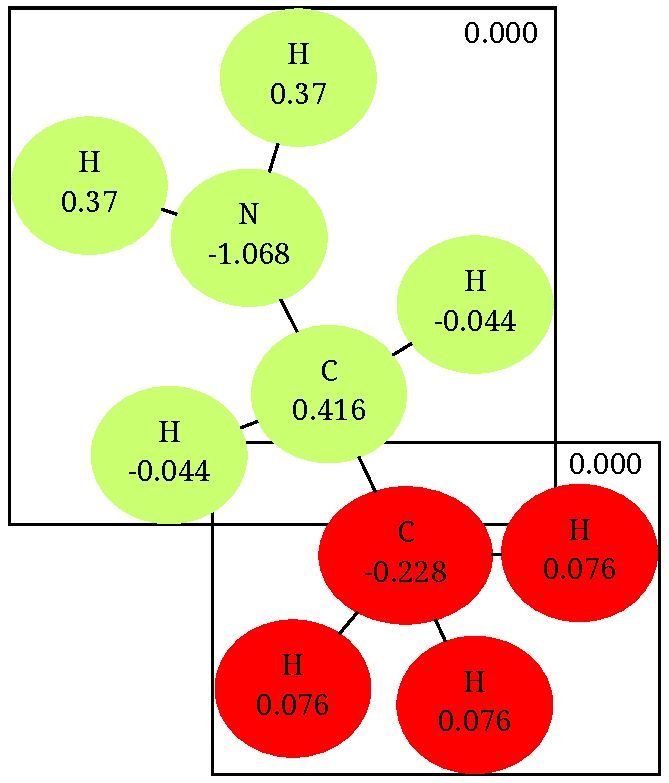
\includegraphics[width=.38\textwidth]{img/ethanamine.pdf}
\caption{Schematic view of ethanamine ($C_{2}H_{7}N$)~\cite{atb2014ethanamine}, including topology data on atom types, atomic charges and charge groups.}
\figlab{partial_charges}
\end{center}
\vspace{-2em}
\end{wrapfigure}

As mentioned in the introduction (\chref{introduction}), biomolecular simulations are becoming increasingly important, especially in the field of drug development. For these simulations, force field models are required to describe the interatomic relations of the drug molecules. In order to run a simulation, these force fields require the molecule's topology. This consists of the molecule's atom types, bonds, bond angles, atomic charges and charge groups.

\Figref{partial_charges} shows a schematic view of an ethanamine molecule. Here, every oval symbolises an atom, and the bonds are displayed as lines between the ovals. The atom type is the letter on the top rule of the oval, i.e.\ there are atoms of type $H$, $N$, and $C$ in the shown molecule. Atomic charges are given by the number at the bottom row~($-1.068$ for the $N$ atom). Finally, the colouring of the atoms and the boxes around them denote a charge group. This is a group of connected atoms, for which the total charge is ideally equal to that of the whole molecule ($0.0$ in this example).

In a recent study, El-Kebir, Klau et al. have developed an algorithm that allows for fast and reliable assignment of charge groups~\cite{canzar2012charge}. As this is now optimised, they currently focus on a different step in the parameterisation: that of calculating the atomic partial charges. Currently, these charges are retrieved using complex quantum-mechanical calculations. However, these calculations can take hours or even days to complete, and cannot be performed for larger molecules. As it is not believed that the algorithms used in these calculations can be improved much further, a different approach is needed for finding atom charges.

\begin{figure}[b!]
\centering
\makebox[\linewidth][c]{%
\begin{subfigure}[t]{0.5\textwidth}
\centering
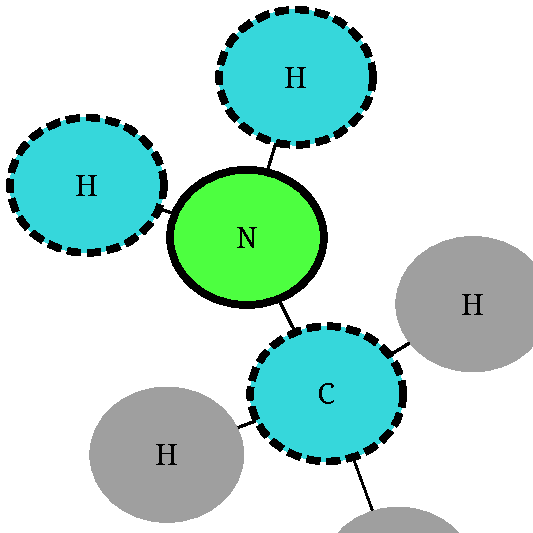
\includegraphics[width=.8\textwidth]{img/match_target.pdf}
\caption{Match target.}
\figlab{match_target}
\end{subfigure}%
\begin{subfigure}[t]{0.5\textwidth}
\centering
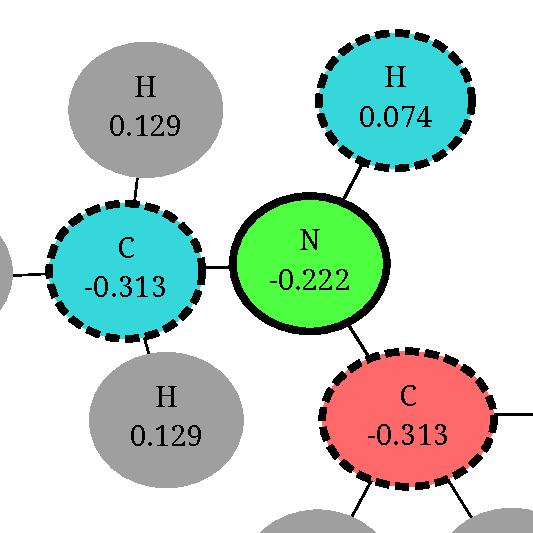
\includegraphics[width=.8\textwidth]{img/match_none.pdf}
\caption{Non-matching fragment.}
\figlab{match_none}
\end{subfigure}%
}\\[1em]
\makebox[\linewidth][c]{%
\begin{subfigure}[t]{0.5\textwidth}
\centering
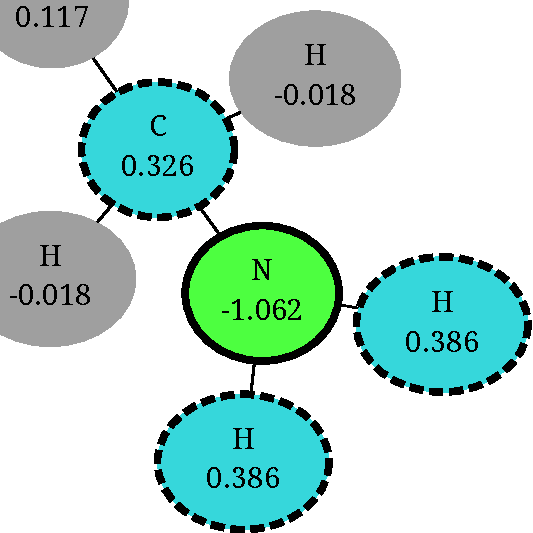
\includegraphics[width=.8\textwidth]{img/match_good.pdf}
\caption{Matching fragment.}
\figlab{match_good}
\end{subfigure}%
\begin{subfigure}[t]{0.5\textwidth}
\centering
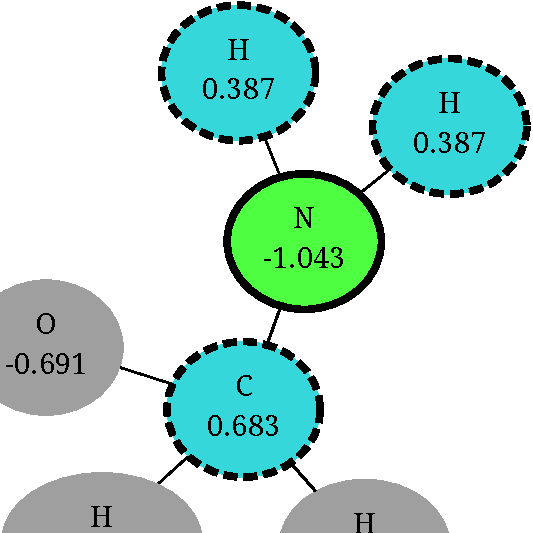
\includegraphics[width=.8\textwidth]{img/match_bad.pdf}
\caption{Matching fragment.}
\figlab{match_bad}
\end{subfigure}%
}
\caption{Basic fragment matching.}
\figlab{matching}
\end{figure}

A possible alternative method of finding atom charges is to exploit the similarity of molecules. The partial charges of an unparameterised molecule can be retrieved from similar fragments of other molecules for which the charges \emph{are} known. In \figref{matching}, the basics of fragment matching are shown. In this case, we are looking for an $N$ atom, with two connected $H$ atoms and a connected $C$ (see \figref{match_target}). As can clearly be seen, \figref{match_none} is not a match, as there are two $C$s connected to the $N$ atom there, and only one $H$. \Figref{match_good, match_bad} show two different fragments that \emph{do} match the target fragment. The $N$ atom is indeed connected to a $C$ and two $H$ atoms in both molecules. We will discuss fragment matching in more detail in \secref{impl_omfraf}.

As can be seen clearly for the $C$ atom in \figref{match_good, match_bad}, charges in similar fragments can still differ. This is due to the fact that atom charges are not only influenced by their direct neighbours, but also by the structure of the rest of the molecule. Due to this, it is not yet possible to fully automate the fragment-based molecule parameterisation process, as there are currently no known rules as to which aspects of the structure influence the charge in which way.

Instead of automating the process, a tool needs to be developed that allows experienced chemists to manually perform the atom charge assignment using fragments of other molecules. This tool should provide them with a list of matching fragments, and leave it to them to find the fragments that properly match with the molecule. In order to do this, users should be able to check all aspects of the found fragments, as these determine whether a fragment is a good match or not. Additionally, they need to be able to easily compare fragments, both with each other and with the target molecule.



\section[Challenges]{Interaction design challenges}
\seclab{id_challenges}
A system for fragment-based molecule parameterisation is not readily available. Therefore, a new system needs to be designed from the ground up. This allows for creating something completely new, but also creates the challenge of doing it right without having any clear starting point. In order to be able to validate the system, we implement two different versions of it and compare them.

Both implementations need to meet the same set of requirements. First of all, the system needs to provide its users with a view of the unparameterised molecule, and help them to find the best matching fragments. As the selected fragments may not always be perfect, it should also be possible for the users to manually adjust the charges for each atom, if they feel that this is needed.

In order to make sure users find the best available matching fragment, they should be encouraged to check as many fragments as possible. However, when many fragments are found, users should not have to compare all of them, as this might cost them way too much time. Therefore, the best matches should be easily recognisable, which requires the found fragments to be presented in a clear and intuitive way.

Another important requirement for the system is that is needs to support parameterisation of both small molecules, consisting of just a few atoms, and large molecules, being over a hundred atoms in size. This means that visualisation of the molecules should be given some thought, in order to make sure both large and small atoms are displayed correctly. It is particularly challenging to find a way to properly visualise large molecules on a screen with a limited size, so an approach is needed that allows for this.

Overall, the most important requirement for the system is to make it work intuitively and to implement it such that it makes chemists' work easier. Parameterising a large molecule should therefore not take hours to complete. Even if that would still be faster than calculating the charges, one can at least do something else while the computations are running. This, of course, is not possible while one has to focus on a manual parameterisation process.

\chapter{Related work}
\chlab{relwork}

This will contain the literature used in this project. It needs to be checked again, cleaned up, updated, and extended.

For this research project, quite a lot of literature is available. The literature has been organised into five different categories, for each of which a number of papers will be discussed.


\section{Molecule simulations}
\seclab{simulations}
Canzar, El-Kebir, et al. discuss their work on charge group partitioning in~\cite{canzar2012charge}. They explain what is needed for running biomolecular simulations and in which steps this information can be gathered. When the atom types, bonds and partial charges of a molecule are known, calculating the charge groups allows for running biomolecular simulations on very small time scales, while still being precise. $\mathcal{NP}$-hardness of the partitioning problem is proven, and an algorithm for quickly calculating the charge groups is presented. The proposed research project is not about assigning charge groups, but the work of Canzar and El-Kebir shows the need for finding the atomic partial charges of a molecule. It also indicates where in the process the partial charges should be calculated, and what will be done with them afterwards.

Malde et al. present the Automated Force Field Topology Builder~(ATB)~\cite{malde2011automated}. The ATB is a web service that can provide topologies for use in molecular simulations. It can both act as a repository for already parameterised molecules and it is able to parameterise molecules itself. This automatic parameterisation involves quantum mechanical calculations, which are very complex and computationally intensive. In the proposed research project, an attempt is made to improve the calculations of atomic partial charges. The results obtained by the tool to be developed will be compared to those obtained by the ATB, in order to validate the value of new tool.


\section{Interaction design}
\seclab{design}
Besides trying to optimise the preparation steps for molecule simulations, the main challenge of this research project is to come up with a good interaction design for a tool that does that. In the interaction design area, Donald Norman is a respected and often cited author. He feels that technology can only live up to its full potential by, first of all, supporting human tasks, while making the supporting technology as transparent as possible by making the tools easy to use, easy to learn and easy to understand. Designing for this purpose is called user-centred design~\cite{norman2002design}.

One of the most important aspects of design is visibility. Every interface should have visible features that can send the right messages to the user. It is very important that user actions do not have coincidental consequences. Otherwise, the user can develop wrong expectations of his actions, which may later result in problems while using the tool. What is also important, is that if a user \emph{does} make a mistake, he should be able to undo this. If this is \emph{not} possible, he may get easily frustrated and will stop using the tool. Finally, the user should not get lost in an enormous list of features. As many of these features will often rarely be used, tools with less features are often the better ones.

An often occurring problem with interfaces is that they get in the way of the task that needs to be performed~\cite{norman1990interfaces}. The user of a tool should not be spending his time `using the interface', but rather on performing the task the tool is supposed to help him with. In order to achieve this, product design should start with analysing the user and the task, and only then designing the user interaction.

When doing interaction design, one has to keep in mind that the appearance of a tool can have a great impact on how well the user of that tool can carry out the tasks the tool is intended for~\cite{norman2002emotion}. Tools that look unattractive tend to focus the mind, which leads to better concentration. For tasks where something needs to be done quickly, this is good, but in cases where creative thinking is required, this will not provide a satisfying result. In that case, the thought processes should be broadened by having something that looks really good. This can easily get the user distracted, which allows for creative thinking.

Not only the appearance of software tools is important, also the form in which the information it comprises is presented can make a big difference. For certain types of data, it is highly beneficial to be represented in a visual form. This allows the viewers to perceive patterns and relationships that might be missed in tables and numbers~\cite{gallopoulos1994computer}. Providing users with the ability to modify view parameters at runtime can increase the benefits even further, as they then have the freedom to explore every aspect of the data. However, these options should not be initially visible, as they are not application specific. As discussed before, these options can cause the application user to get lost in the list of options, no longer being able to execute the task he wants to perform. Therefore, the options should be located in some initially closed menu.

Despite the fact that the importance of design has been long known, many software products are still poorly designed. In an attempt to overcome this, an approach called human-centred design (HCD) has been developed~\cite{norman2005human}. However, even though the needs of the user play a central role here, many companies following the HCD principles still develop complex and confusing products. The systems are often superb at the level of the static, individual display, but fail to support the sequential requirements of the underlying tasks and activities. Therefore, a new approach is needed that does not put the user in a central role, but rather does so with the activity that needs to be performed. In this activity-centred design method, it is sometimes necessary to ignore a user's requests as they might compromise the task that has to be carried out.

This, however, does not mean that the application user's needs should be completely ignored. On the contrary, it is really important that the user's characteristics are understood and used in the design of an application~\cite{badre2002shaping}. Also, a good analysis of the context is needed to make the right design decisions. If one ignores the user characteristics and context of an application, the application is  likely to fail, as the context in which the application is developed will almost always differ from the context in which it will be used.

\subsection{Learning}
\seclab{id_learning}
Before we can determine what makes a good interaction design, we need to know something about how people learn new things and how our problem solving system works. There are two main learning mechanisms: schema acquisition, where knowledge of subject matter is organized in schemas that determine how new information is dealt with, and the transfer of learned procedures from controlled to automatic processing~\cite{sweller1994cognitive}. Well learned material can be processed automatically, without much effort, while new or less familiar information needs to be processed in a controlled fashion. This means that, when learning something new, one can only use that knowledge by devoting considerable cognitive effort to it. After getting more familiar with the task, the skill may become automatic. Only then can intellectual performance attain its full potential.

In order to facilitate learning, the process of schema acquisition needs to be triggered and supported. Trying to teach by only providing examples will eventually even have the opposite effect. The learner will then be able to execute the task under the conditions that are equal to those in which he learned the skills, but will fail to do so in other cases. In order to overcome this, teaching should be done using goal-free problems. These problems focus on achieving various problem states and the steps on how to get there, which is exactly how schema acquisition works.

How easy it is to learn something new is highly dependent on the level of interactivity between the different elements of a task. If there is no interaction between two elements, they can be learned in isolation, requiring less cognitive load then when they have to be learned simultaneously. However, making something easy to learn is not as simple as reducing the element interactivity, as it is dependent on the knowledge of the individual what constitutes an element. For the more experienced, this may be a whole chunk of the information, while for the rest an element may be an atomic part of the information. Luckily, it is only hard to learn something new when both the intrinsic and extraneous cognitive loads are high. When there is only one high load, the lack of the other compensates for this.

There are two types of problems: well-structured problems and ill-structured problems. In a well-structured problem, the initial state is well-defined, the goal state is known, and there is a limited set of logical operations to solve the problem~\cite{jonassen2000toward}. If either of these is missing, the problem is classified as being ill-structured. Ill-structured problems are generally more complex than well-structured problems, and are therefore often harder to solve.

Besides the complexity, there are also many individual differences that determine how easy it is to solve a problem. First of all, when a person is familiar with the domain of a problem, it will be easier to solve for him than it will be for someone with less domain knowledge. Second, more analytical thinkers are often good problem solvers. They must believe that there will be a way to solve the problem, especially when the problem is ill-structured, as they might otherwise just give up before finding a solution. It also helps when someone has a certain affection with the problem. He will then be more likely to try and find the solution. If, however, one has certain beliefs or attitudes about a problem and its solution, he might be a less effective problem solver due to over-relying on that solution. Finally, every problem is different and requires different skills to solve. It can be easier to solve the problem for someone who is familiar with the problem type, but one may never forget that every problem requires a different way of learning.

\subsection[Principles]{Interaction design principles}
\seclab{id_principles}
Following the previously discussed and other research, a number of principles of interaction design can be identified. However, different authors have different opinions on what those principles are. Norman and Nielsen identify the following principles of interaction design that are completely independent of technology~\cite{norman2010gestural}:
\begin{itemize}[noitemsep,topsep=0pt,parsep=0pt,partopsep=0pt]
\item Visibility (also called perceived affordances or signifiers);
\item Feedback;
\item Consistency (also known as standards);
\item Non-destructive operations (hence the importance of undo);
\item Discoverability: all operations can be discovered by systematic exploration of menus;
\item Scalability: the operation should work on all screen sizes, small and large;
\item Reliability: operations should work and events should not happen randomly.
\end{itemize}
Thimbleby, on the other hand, \emph{does} relate his principles to technology~\cite{thimbleby2007press}:
\begin{itemize}[noitemsep,topsep=0pt,parsep=0pt,partopsep=0pt]
\item Use good algorithms for better user interfaces: interactive devices are designed to solve problems in a structured way, which is exactly what a good algorithm does;
\item Use simple, explicit interaction frameworks: those provide clear interaction structures, which allow for reliable feature integration, checking, analysis, fault identification, and error fixing;
\item Interrelate all interaction programming: all aspects of the design should come out of the same specification;
\item Define properties and analyse designs for them.
\end{itemize}
A more extensive list is provided by Blair-Early and Zender~\cite{blair2008user}:
\begin{itemize}[noitemsep,topsep=0pt,parsep=0pt,partopsep=0pt]
\item Obvious start: design an obvious starting point;
\item Clear reverse: design an obvious exit or stop;
\item Consistent logic: design an internally consistent logic for content, actions, and effects (the most important consistency is that with user expectations);
\item Observe conventions: identify and consider the impact of familiar interface conventions;
\item Feedback: design tangible responses to apt user actions;
\item Landmarks: design landmarks as a reference for context;
\item Proximity: design interface elements in consistent proximity to their content objects and to each other;
\item Adaptation: design an interface that adapts or is adapted to use;
\item Help: as necessary, provide a readily accessible overall mechanism for assistance;
\item Interface is content: design interface elements that minimise interface and maximise content.
\end{itemize}

The above lists of principles are all quite different, but all consider automation of certain processes. The next section will discuss this in more detail.

\subsection{Automation}
\seclab{id_automation}
Software and artificial intelligence developments allow for increasing possibilities in automating processes. The amount of interaction between humans and computers can be reduced, allowing humans to concentrate on other tasks~\cite{payne2000varying}. However, it depends on the situation when automation should be applied and to what extent. Automation reduces people's situational awareness, which might be unwanted in some environments. Furthermore, it may leave users feeling out of control or lead to deskilling if decisions are being made automatically, rather than just giving advise.

In order to determine what level of interaction is suitable for a task, multiple interaction methods need to be designed. These often include a `naive' version that only does validation of user input, a `cooperative' version in which the user is given advise on what to do, and a mostly automatic `autonomous' version that only requires some parameterisation. In a case study on route planning agents it was found that, for that purpose, the cooperative version delivered the best results. The users of the autonomous version complained they lacked the possibility to fully control the system, while those who used the naive version complained the route planning process was tedious. However, this does not mean that the cooperative version is the silver bullet for man-machine interaction. In some cases, having full control might be necessary, or in other cases, where time consumption is really important, the autonomous version might be preferred.

Cooperative or mixed-initiative user interfaces have been studied in more detail by Horvitz~\cite{horvitz1999principles}. He has found that in order for automation to work, automated activity should not occur before a user is ready for it, but also that delays in automation can diminish its value. Among the most important factors for successful semi-automatic applications are: considering the computer's uncertainty about a user's goals, inferring the ideal action in light of costs, benefits and uncertainties, minimizing the cost of poor guesses, and providing mechanisms for efficient agent-user collaboration to refine results.

An example of a system that has implemented this cooperative interaction design is \verb|SALT|~\cite{marcus1987taking}, a tool for generating expert systems to be used in problem solving. Using \verb|SALT|, one will incrementally construct a design by either accepting or rejecting proposed design parameters, one parameter at a time. Constraints will constantly be checked, and, once a constraint violation is detected, the system will try to automatically remedy this. As it is extremely difficult to develop a system that has to perform a task for which expert knowledge is required, \verb|SALT| offers ways to backtrack the assigned design parameters. It will automatically detect parameters that might need to be modified, but require additional domain knowledge to be done properly.

At every step in \verb|SALT|'s incremental parameter assignment, the proposed values are given in such order that the ones having the least negative effect come first. However, as this does not consider future assignments of other parameters, this means that the assignment may not always converge to a proper solution. This is where the previously discussed backtracking will be useful to see where the `wrong' decision has been made. In two field studies, \verb|SALT| has been proven a good and useful tool for problem solving. However, it has also been found that the required degree of interaction can vary among different systems. Therefore, one should always study the context of a system before deciding on the level of interaction that system will have.

Automation is often said to be causing problems and to increase the chances for human error when failures occur. Norman proposes in~\cite{norman1990problem} that this is not the cause of automation itself, but rather of the automated systems' lack of appropriate feedback when humans need to take over control. In regular conditions and some predefined exceptional situations, automated systems are perfectly able to operate. It is in those other abnormal situations that automated systems often fail; both in executing their task and alerting the user that something unusual is happening. In order to overcome this, automated systems should be designed while keeping in mind that errors will occur. An appropriate feedback system needs to be present that allows for human intervention when needed.

An often used, but wrong way of alerting a system's user something is wrong is the use of alarms for every component of the system. In exceptional situations, multiple components will often fail at the same time. When all of these would sound an alarm, the user could get confused and will not know what component requires immediate attention and what can wait. Rather than this, systems should continually inform the user about their state, such that he can detect exceptional situations and act upon them. Still, this information should be non-intrusive and presented in a natural way, such that man and machine can jointly solve the problem at hand.

\subsection{Abstraction}
\seclab{id_abstraction}
In order to be able to say something about an interaction design, this design needs to be represented at an abstract level. In~\cite{brehmer2013multi}, Brehmer and Munzner describe a multi-level typology for visualisation tasks. This typology consists of the answers to three questions: \verb|why| the task is performed, \verb|how| the task is performed and \verb|what| it pertains to. A list of predefined nodes is provided with which those questions must be answered. By comparing multiple of these typologies, one is able to reason about the differences between two systems on an abstract level, which can be used to hypothesise what system will work better under which circumstances.


\section{Molecule software}
\seclab{software}
There is a lot of software available for displaying, drawing and editing molecules. These programs form an indispensable part of every molecular processing system~\cite{ertl2010molecular}. Throughout the years, these programs have evolved from basic text editors, through clickable image maps, to full-on molecular structure sketching software. In the last few years, a new trend becomes visible. More and more cheminformatics applications are being brought to the web, allowing for a lot of new ways of interaction. Furthermore, these new applications are being open sourced, allowing for new innovative variations or combinations of the old tools.

An example of a previously offline, closed source tool is \verb|JSmol|, previously known as just \verb|Jmol|~\cite{hanson2013jsmol}. This tool has been seamlessly transformed from a \verb|Java| applet to \verb|JavaScript|, without any visible visual difference. Furthermore, performance wise, there is only a minor difference between the two implementations. Another example is \verb|JSME|~\cite{bienfait2013jsme}. This tool has even been cross-compiled from its original \verb|Java| code to \verb|JavaScript| using the \verb|Google Web Toolkit| compiler. The transition to the web has resulted in the addition of several features, suggested by users from the new, bigger audience. What can be concluded from these two cases is that bringing molecule software to the web opens up a whole world of new possibilities, without having to give up on performance.

With the ongoing migration of molecule software to the web, new devices, such as smartphones and tablets, will be able to run the tools. As these devices promote different ways of user interaction and often have smaller screens, designs of the molecule software need to be reconsidered. \verb|TB Mobile| is a mobile app for identification of potential anti-tuberculosis molecules~\cite{ekins2013tb}. The app is structured in such way that there is always a small control bar at the top, and a large area for showing the content. Interaction with the app is handled by a small number of large buttons, allowing for easy touch controls. In order to work for different screen sizes, everything in the content area is scalable, and, in case not everything fits on the screen, scrollable. Usage of the app in practice has shown that it helps to improve the work flow of tuberculosis researchers, by lowering the barriers for accessing the information it provides.

The issue of showing a lot of data on a limited-size screen is also addressed by Ertl and Rohde~\cite{ertl2012molecule}. They took the concept of a word cloud, and transformed that to a molecule cloud, where the highest scored molecules are the biggest and the lowest are the smallest. None of the molecules overlap, and the sizes are divided such that the whole available screen space is filled. User studies have shown that these molecule clouds provide an easy way of finding the most relevant molecules. In the proposed research project, this may be useful for showing the set of related fragments of other molecules, depending on the size of that set.


\section{User studies}
\seclab{user_studies}
In Software Engineering, an often used method to evaluate a project is performing a user study. In general, user studies can be assigned to one of the following categories: experiments, case studies, surveys, and post-mortem analyses~\cite{wohlin2003empirical}. In all of these types of studies, it is important to have a representative group of test subjects. These should preferably be picked at random from the population of application users.

This project, first of all, will subject a number of users to an experiment. In an experiment, two (or more) different configurations of the examined tool are compared by examining the effects the configuration has on the tool's output~\cite{wohlin2003empirical}. It is important to define exactly what one wants to validate~\cite{stein2009assessing}. This should preferably be something that can easily be observed (e.g. `time required' or `number of clicks', but not `comprehensibility'). Furthermore, it is important that all different configurations are semantically equivalent (i.e. doing the same thing), have an equal degree of compression (i.e. contain the same information) and formatted into their cleanest and clearest extent.

Before starting an experiment, it is very important to make sure your subjects are committed to the tasks they need to perform. Otherwise, the experiment will not properly reflect the production environment. Furthermore, the experiment should be well-prepared, as start-up problems might negatively impact the subject's opinion otherwise.

Besides the experiment, this project will also contain a survey. In a survey, it is easy to test a large number of variables, but one should be careful not to test too many, as this will make the analysis infeasible~\cite{wohlin2003empirical}. In order to collect questionnaire information in a structured way, its questions should follow some natural flow that embodies all aspects of a user's experience~\cite{tuch2013analyzing}. This encourages them to report their detailed experiences, as this is less demanding than answering one big open question. Furthermore, it also reduces the chances of subjects failing to report certain things, simply because they forgot about them.

A few predefined surveys are available for usability testing, including \verb|SUS|~(System Usability Scale) and \verb|UMUX|~(Usability Metric for User Experience)~\cite{lewis2013umux}. \verb|SUS| consists of ten items, each of which should be graded on a scale of 1 (strongly disagree) to 7 (strongly agree). It has been extensively tested and turns out to have a reliability score of 0.96. \verb|UMUX| is a shorter questionnaire, consisting of four questions, but its even shorter brother, \verb|UMUX-LITE|, consisting of only two questions, has been shown to provide results of the same reliability as \verb|UMUX|. When a system is subjected to both \verb|SUS| and \verb|UMUX-LITE|, one can get very reliable results on the usability of that system.

On a final note about surveys, the fact that they are often straight-forward makes them perfectly suitable for being held over the internet. It has been shown that the results of online surveys do not significantly differ from their offline counterparts~\cite{komarov2013crowdsourcing}. However, face-to-face surveys are still the only way that allows both the interviewer and the test subject to immediately ask and answer questions~\cite{wohlin2003empirical}. Even if this does not lead to a significant difference in the outcome of the survey, it can definitely lead to new insights.

Before analysing the data obtained by a user study, it is important to validate it~\cite{wohlin2003empirical}. All the obtained results should be complete and correctly documented. Furthermore, extreme outliers should be identified dealt with. What should happen exactly depends on the situation, but in most cases it is best to leave out the extreme results~\cite{komarov2013crowdsourcing}. Finally, it is very important to provide a grade of validity along with the conclusions of the user studies. This grade depends on, for instance, the number of test subjects, their representativeness or the distribution of the results.

\chapter{Research approach}
\chlab{approach}

In this project, as discussed before, we design and implement a tool for fragment-based molecule parameterisation, in order to answer the research questions that were discussed in \secref{id_questions}. In the current chapter, we discuss the taken approach. 

Since the idea of fragment-based molecule parameterisation is a new concept, it comes as no surprise that there are no existing tools for this. Furthermore, no tools exist that allow for easy comparison of molecules, or molecule fragments, either. This means that there is no baseline to which the developed tool can be compared. In order to still be able to say something about the quality of the tool, we make two different implementations of it~(see \secref{ra_versions}).

In order to evaluate the two implementations, both of them are subjected to a user study~(see \secref{ra_studies}). This will help to determine if the system works properly and whether it is fit for its tasks. Furthermore, this allows us to answer the project's research questions, and test the hypotheses that will be discussed in \secref{ra_hypotheses}.



\section{Two versions}
\seclab{ra_versions}
There are a few axes along which the differences between the two implementations can be made. One could, for instance, compare two tools with varying visualisation methods. Visualising molecules, however, is a well-exhausted field of research, leaving very little room for new ideas.

Another possible variable in the tool is the way its users will interact with it and especially its degree of automation. Varying this degree has been the subject of several studies~(e.g.~\cite{payne2000varying, horvitz1999principles, marcus1987taking, norman1990problem}, see also \secref{id_automation}), all of which concluded the degree to which automation can be applied is highly dependent on the context of the system and sometimes even to the situation in which the system is used.

As discussed in \secref{id_automation}, usually three levels of automation are implemented, creating a naive, cooperative and autonomous version of the system~\cite{payne2000varying}. As it is considered hard to parameterise a molecule based on fragments of other molecules, and little is known on what is the best way of doing this, an autonomous version of a tool that does this cannot yet be developed. The other two versions, however, seem to be perfectly implementable and both can be considered useful.

We have therefore decided to implement a naive version of the system that has barely any automation at all, and a cooperative version that will continuously make suggestions to the user. We will call them the \IDa\ and \IDb\ version respectively, to reflect on the fact that the \IDa\ version only reacts to user input, whereas the \IDb\ version proactively guides the user through the process by continuously making suggestions~(see \secref{id_versions}). Note that the names reflect the system, \emph{not} its user (i.e.\ the reactive system is used proactively by the user, and vice versa). The interaction designs for these two versions are discussed in detail in \chref{design}.



\vspace{-.2em}
\section{User studies}
\seclab{ra_studies}
\vspace{-.2em}
As mentioned before, both versions of the developed system are evaluated in a user study. Unfortunately, we cannot just ask anyone partake in this experiment, as it is a system that is aimed to be used by experienced chemists who understand the details of molecule parameterisation. Luckily, project supervisors Klau and El-Kebir keep a close connection with a substantial group of chemistry researchers, creating the opportunity of asking them to participate in a user study. They are interested in the concept of fragment-based molecule parameterisation, and willing to test a system that does that.

In the user studies, the participants are split up in two groups, where each person is randomly assigned to a group and both groups are of equal size. This way, it is made sure that both groups are representative, which is essential for user studies~\cite{wohlin2003empirical}~(see also \secref{user_studies}). The groups take part in an experiment that compares the two versions of the molecule parameterisation tool. Due to the limited number of test subjects, every participant is asked to test both the \IDa\ and the \IDb\ version of the system. As the effects of the order in which two systems are evaluated are often remarkable, one group starts the evaluation with the \IDa\ version, followed by the \IDb\ version, while the other group does this the other way around.

For both versions of the tool, the experiment participants are instructed to parameterise a couple of molecules. After this, they are asked to fill in a short questionnaire containing questions about that specific version of the system. When they have tested and answered questions about both versions of the tool, users are asked to submit one final questionnaire. This one contains more general questions about having a system for molecule parameterisation, and asks for their preferred version.

Due to the large number of tasks the experiment participants have to complete, we have decided to have them parameterise only 2 molecules per version of the system, i.e.\ 4 molecules in total. With an estimated time requirement of 10 minutes per questionnaire, participants are already spending half an hour on that. As the experiment should not take up more than an hour of the participants' time, this leaves only 30 minutes for the actual molecule parameterisation. When loading times are considered, we must conclude that there is only time for 4 molecules in total.

Even though testing more than two molecules per version of the system would be better, it is not necessarily a problem to only test two. Many problems with a system will be found in the first two test runs, after which the number of newly discovered problems decreases rapidly~\cite{krug2006dont, nielsen2000you}. Despite the fact that some problems may be left undiscovered, the most common flaws will usually be spotted in the first few runs.

As many of the available participants are scattered around the world, and in order to save time, we have decided to conduct the experiment over the internet. The potential application users are contacted via email, and instructed to use their own machines to run the system. Additionally, they submit the answers to the questionnaires using some online form.

In order to be able to obtain usage statistics from the user studies, an extensive logging mechanism needs to be built into the system. Later, this can be used to precisely reproduce the user's actions. This mediates the loss of information due to the fact that the user studies are performed over the internet, with no human observing the participants. If any odd results are found, the logs can potentially help to pinpoint what went wrong, and, more importantly, they can be used to obtain all kinds of statistics about the molecule parameterisation system.



\section{Hypotheses}
\seclab{ra_hypotheses}
According to Jonassen's dichotomy of problems~\cite{jonassen2000toward}~(see also \secref{id_learning}), fragment-based molecule parameterisation is an ill-structured problem. This means that the problem is quite complex and is therefore hard to solve. Due to this, users need to be ensured that there is a way to find a solution, or they will simply give up. This should be the case for both versions of the system, but is better facilitated by the \IDa\ version than the \IDb\ one. In the \IDa\ version, users are not relying on a system to automatically come up with suggestions, but rather do everything themselves. They will know that, by simply repeating the same process a few times, they will get a result. The fact that they have everything in their own hands will make them feel more comfortable about getting to a good solution.

In the earlier mentioned study of Payne, Sycara, and Lewis~\cite{payne2000varying}, it was found that the cooperative version of the examined system had great benefits in time consumption and user guidance, where the naive version excelled in user freedom. In the general, straight-forward cases studied there, the cooperative version delivered the best results, but, in more complex situations, it was no match for the naive version. As fragment-based molecule parameterisation is an ill-structured, and therefore complex problem, we believe that the following hypotheses hold:
\begin{quote}
The \IDb\ version of the molecule parameterisation system takes less time to use than the \IDa\ version.
\end{quote}
\begin{quote}
The \IDa\ version of the molecule parameterisation system yields better results than the \IDb\ version.
\end{quote}

When the participants of the study on automating RPAs~\cite{payne2000varying} were asked what they thought about the different versions of the system, they noted that using the naive version was a tedious process that cost a lot of time. However, in some more complex cases, they found it really important to have full control of the system. As mentioned before, parameterising a molecule based on fragments of other molecules is a complex task in itself. Therefore, as we consider user satisfaction and result correctness to be the most important aspects in this case, we formulate the following hypothesis about the system in general:
\begin{quote}
For a tool used for fragment-based molecule parameterisation, it is better for users to have full, manual control, than to automate certain parts.
\end{quote}

On a more general level, both versions of the interaction design rely on the idea that fragment-based molecule parameterisation should be chemically correct. As this has not been proven yet, we aim to determine if it is possible at all. Both versions of the system are designed in such way that the user should be able to quickly parameterise a molecule. Furthermore, as it has been proven that properly matching parts of molecules have the same atomic charges, the second, for both versions of the system essential hypothesis, is as follows:
\begin{quote}
It is possible to parameterise a molecule based on fragments of other molecules; both accurately and in a reasonable amount of time.
\end{quote}

When this hypothesis does not hold, fragment-based molecule parameterisation will show not to be a good concept after all. This will also render the comparison of the two interaction designs invalid, as both are then designed for a faulty task, and have been evaluated using that. We consider it very unlikely that this would happen, since the similarity has been proven in theory, and the parameterisation times cannot get much worse than those of the quantum-mechanical calculations.

\chapter{Interaction design}
\chlab{design}

As discussed before, there is no existing software for fragment-based molecule parameterisation, which means that there are no existing interaction designs for such systems either. What does exist is a wide range of tools and programs for visualising, creating and editing molecules. This includes stand-alone molecule drawing software such as \verb|Accelerys Draw|~\cite{accelrys2012accelrys}, \verb|Avogadro|~\cite{hanwell2012avogadro}, \verb|PyMOL|~\cite{delano2002pymol}, and \verb|RasMol|~\cite{pembroke2000bio}, two-dimensional web based molecule editors like \verb|ChemDoodle 2D Sketcher|~\cite{ichemlabs2013chemdoodle}, \verb|Marvin4JS|~\cite{chemxon2013marvin}, and \verb|Molsoft HTML5 Molecule Editor|~\cite{molsoft2012molsoft}, and online three-dimensional visualisation tools \verb|CanvasMol|~\cite{altered2013canvasmol} and \verb|JSMol|~\cite{hanson2013jsmol}.

These existing tools will serve as an initial guideline for the interaction design of the molecule parameterisation system that is to be developed. Combined with the basic interaction design principles as posed by Norman and others~(see \secref{design}) and the knowledge gathered in earlier studies on molecule software~(see \secref{software}), it should be possible to design the system such that it meets its requirements~(as stated in \chref{analysis}). In the remainder of this chapter, we discuss such interaction design.



\section{Platform}
\seclab{platform}
Over the past few years, there has been a trend in bringing everything to the web~\cite{ertl2010molecular}~(see also \secref{software}). Following this trend, it has been decided to implement the front-end of the molecule parameterisation system as a web application. This allows the system to run on any desktop and laptop operating system, and creates the possibility of running it on a smartphone or tablet\footnote{This, however, is not a requirement for the system.}, without requiring any modifications. Having the user interface as a web service means that the back-end, where the actual finding of matching fragments occurs, needs to be available through the web as well.



\section{Two versions}
\seclab{id_versions}

\begin{figure}[h!]
\begin{center}
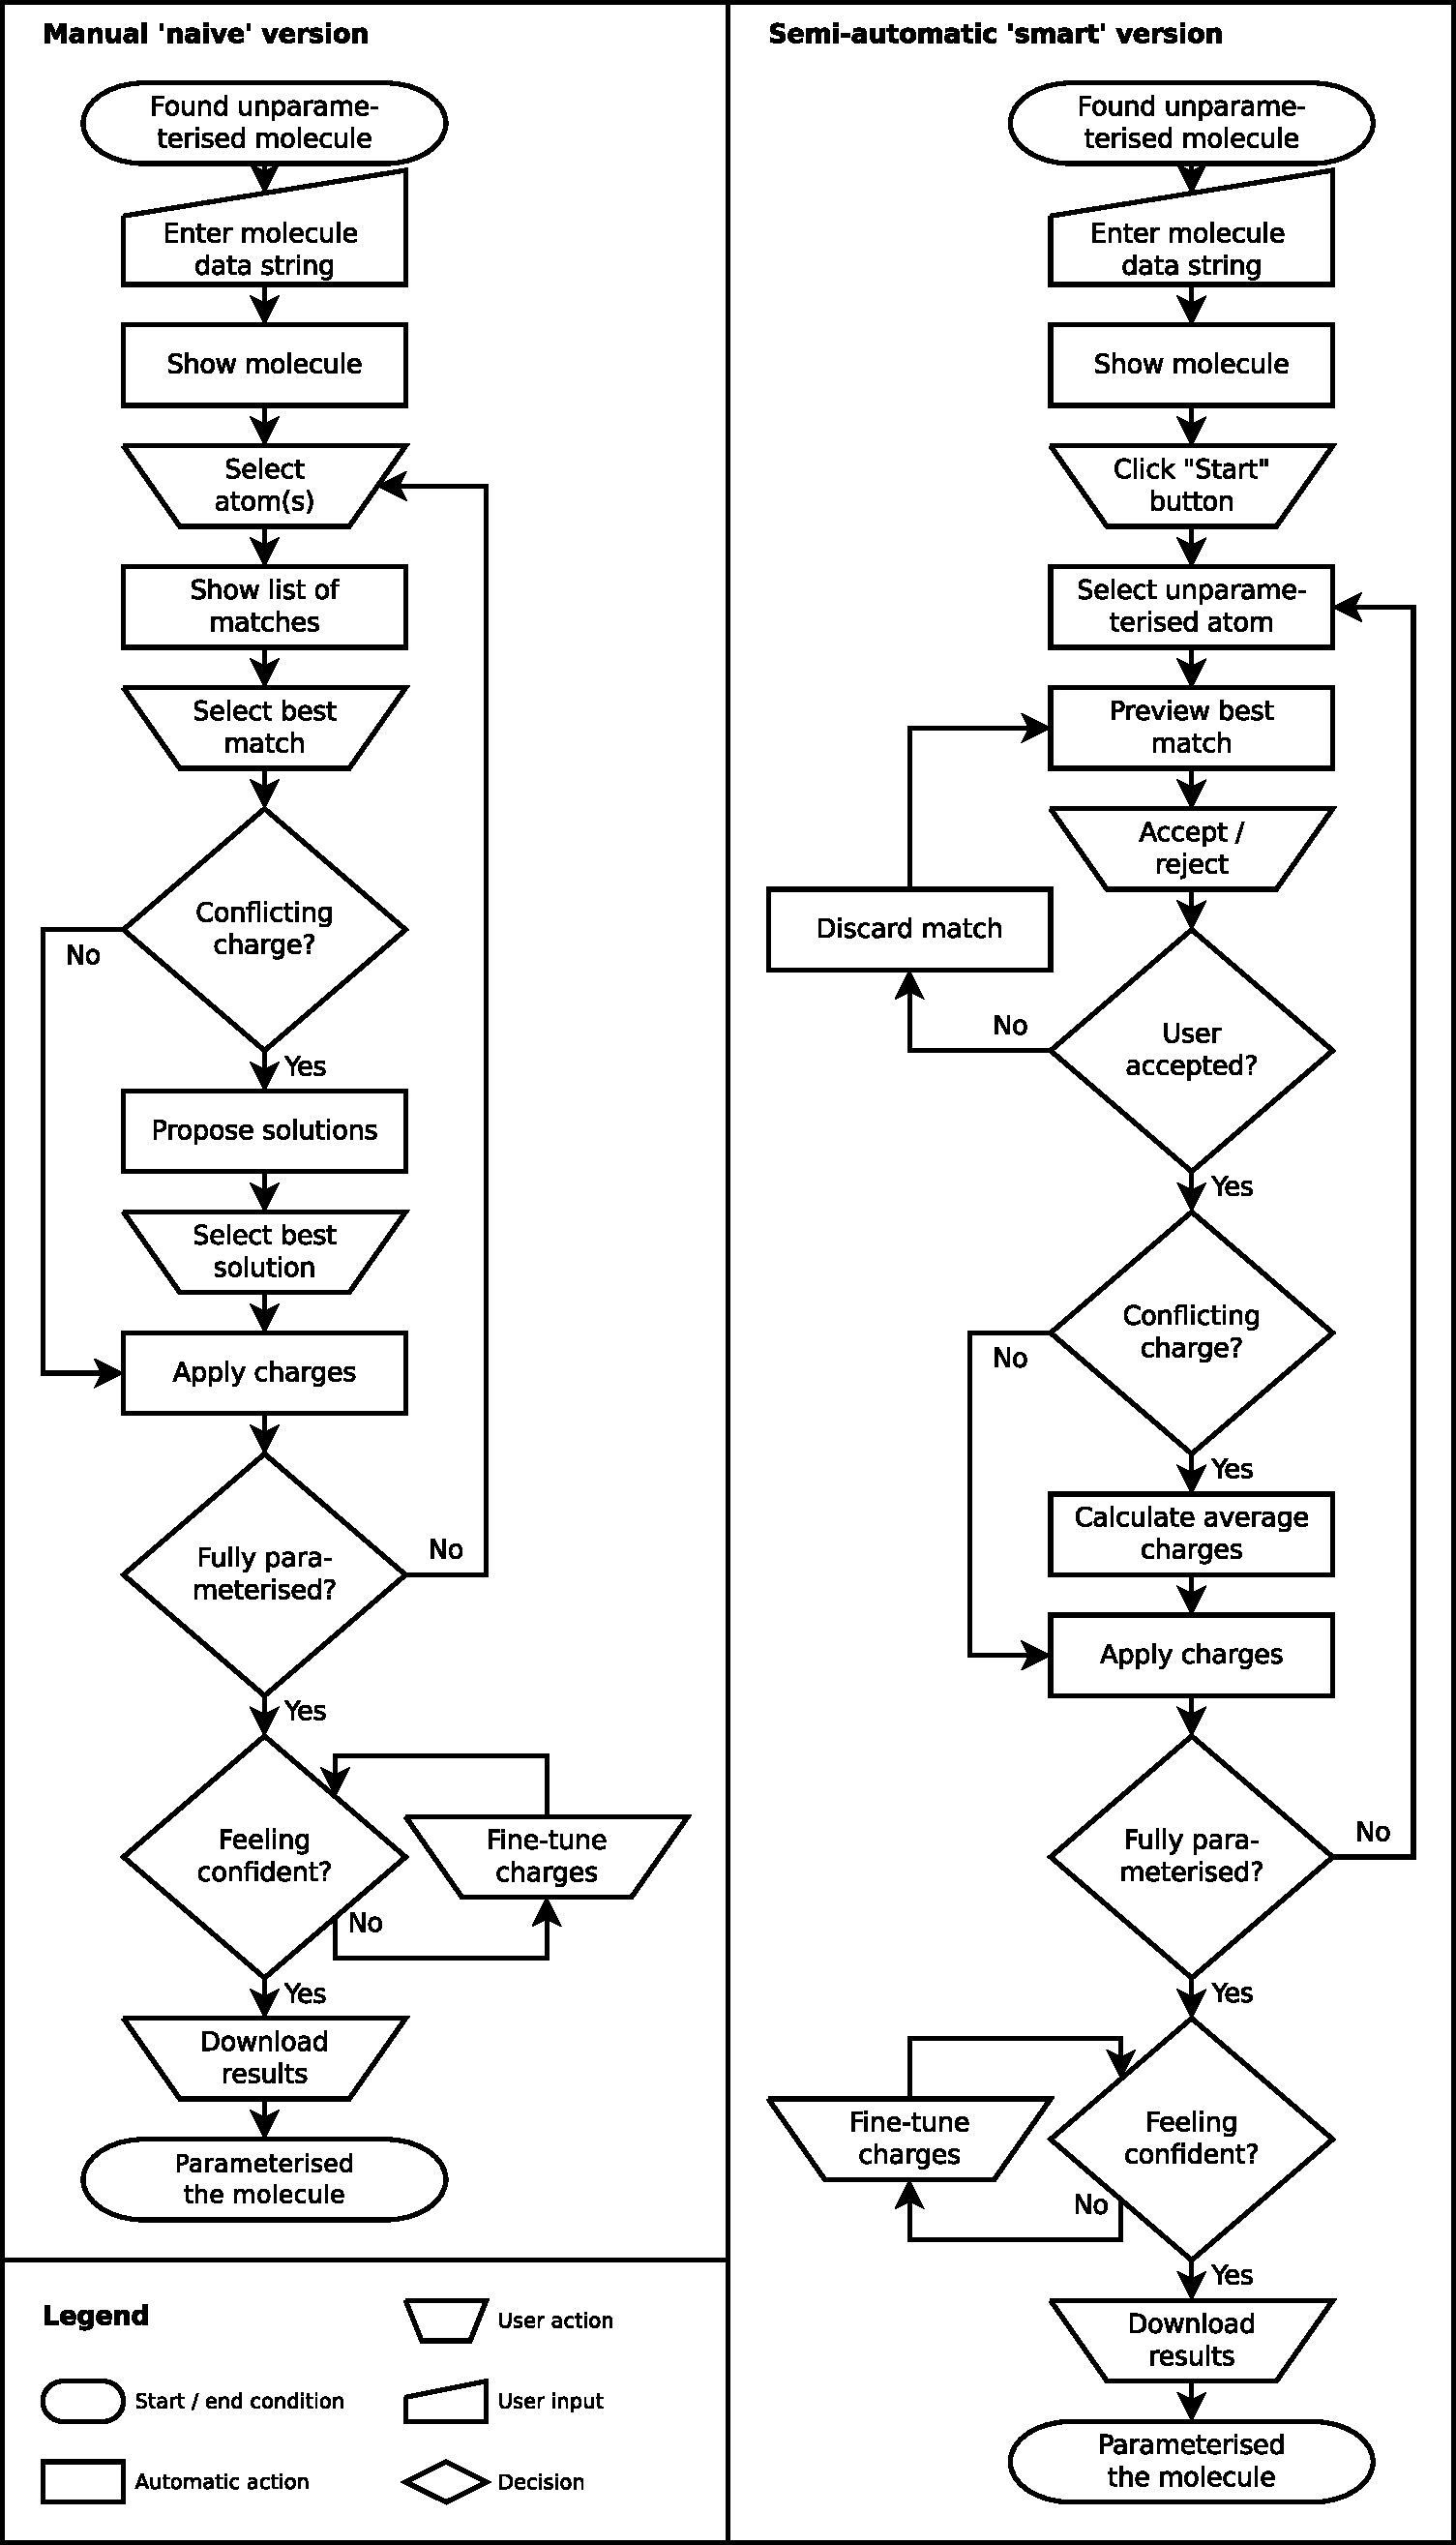
\includegraphics[width=.9\textwidth]{img/complete_id.pdf}
\caption{Sequence diagram for the two different interaction designs.}
\figlab{id_flows}
\vspace{-2cm}
\end{center}
\end{figure}

As discussed in \secref{ra_versions}, two different versions of the molecule parameterisation system need to be implemented, with varying levels of automation. This means that two different interaction designs need to be made as well. \Figref{id_flows} shows a version where the user has to manually do the whole parameterisation, and a semi-automatic one which continuously makes suggestions to the user. These manual and semi-automatic versions have been called consuming and producing respectively. In the consuming version, the system only does what the user tells it to do. It does not give any suggestions, and only consumes user input. The producing version, on the other hand, \emph{does} continuously make suggestions, i.e.\ it automatically produces parameterisation previews~(see also \secref{id_comparison}). The following sections will discuss these two interaction designs, the motivation behind them, and their workings.


\subsection{Commonalities}
\seclab{id_common}
As can be seen in \figref{id_flows}, the two interaction designs share a common start and ending. First of all, the user will need to find a molecule that he wishes to parameterise. The molecule then needs to be inserted into the system, for which the user needs to find a representation of the molecule that the system can work with. It has been decided that this so called molecule data string~(MDS) needs to be in the \verb|SMILES|~\cite{daylight1992daylight}, \verb|InChI|~\cite{heller2013inchi}, or \verb|PDB|~\cite{bernstein1977protein} format, as these are the most commonly used.

Many users of the system will be familiar with the ATB~\cite{malde2011automated}~(see also \secref{simulations}) and will probably find the molecules they want to parameterise in the ATB repository. Therefore, it should also be possible to use an \verb|ATB molecule ID| as input for the system. From that \verb|ATB ID|, the corresponding \verb|PDB| structure file can be retrieved from the ATB servers, which can then be used in the rest of the process.

After the molecule has been shown to the user, the two versions of the interaction design start to differ. This will be discussed in more detail in the following sections, where \secref{id_naive} discusses the consuming version, and \secref{id_smart} describes the producing interaction design.

As soon as the molecule has completely been parameterised, the two interaction designs join the same path once more. The user now has the possibility to manually fine-tune the charges, if he feels that this is needed. This can be done by selecting an atom and clicking an ``Edit charge'' button. In order to assist the user in finding a proper charge for the atom, the molecule fragments that have been used to get the current charge can be displayed. As soon as the user feels the assigned charges are correct, he should be able to download a file containing the results of the parameterisation.

In order to reduce the effect of user mistakes on the parameterisation process, every user action can be undone, including the undo action itself. This way, the user does not need to start over completely when he makes a small mistake, such as accidentally selecting the wrong fragment. It also allows for more experimentation, as there are no definitive consequences of any user action~\cite{norman2002design,norman2010gestural}~(see also \secref{design}).


\subsection{Consuming version}
\seclab{id_naive}
Just like the naive RPA implementation from~\cite{payne2000varying}, the only automatic process occurring in the consuming version of the molecule parameterisation tool is the validation of user input. Besides ordering the matching fragments based on their probability of being a good match, the tool will not give any advise, nor will it automatically infer any values.

\subsubsection{Operation}
The operation of the consuming version of the tool is shown in \figref{id_flows}. In more detail, the complete set of steps required to fully parameterise a molecule is as follows:
\begin{enumerate}[itemsep=.1em, parsep=.2em, topsep=0em]
\item The user enters a molecule data string (in \verb|SMILES|, \verb|InChI|, \verb|PDB| format, or using an \verb|ATB molecule ID|). The molecule will be displayed to the user;
\item The user selects a single atom or a group of \emph{connected} atoms. They need to be connected, since non-connected atoms have different characteristics;
\item A list of matching fragments will be loaded and shown, ordered by decreasing rating. The user can browse through them, preview the result of selecting that match and, once he has found what he sees as the best available match, select this one;
\item
  \begin{itemize}[leftmargin=0cm, itemsep=.1em, parsep=.1em]
  \item[] {\bf Fragment only contains unparameterised atoms}:\\
    The charges from that fragment are assigned to the molecule;
  \item[]{\bf Fragment contains parameterised atoms}:
    \begin{enumerate}
    \item
      Details of the charge conflict are shown, along with the a list of possible solutions. The user picks one of the following solutions:
      \begin{itemize}[itemsep=.1em, parsep=.2em, topsep=0em]
      \item Take the average of the two charges;
      \item Keep the current value;
      \item Take the new value;
      \item Manually enter a value.
      \end{itemize}
    \item The solution is applied and the resulting charges are assigned to the molecule.
    \end{enumerate}
  \end{itemize}
\item
  \begin{itemize}[leftmargin=0cm, itemsep=.1em, parsep=.1em]
  \item[]{\bf Unparameterised atoms remain}:\\The user selects another atom / list of connected atoms. Back to step 2;
  \item[] {\bf Molecule fully parameterised}:\\Continue to step 6;
  \end{itemize}
\item
  \begin{itemize}[leftmargin=0cm, itemsep=.1em, parsep=.1em]
  \item[] {\bf User feels charges need to be fine-tuned}:
    \begin{enumerate}
    \item The user selects the atom whose charge he wants to modify;
    \item The user clicks the ``Edit charge'' button for that atom;
    \item The user can now view the fragments that were used to find the charge for this molecule. Using that and potentially other information, he can find a better charge for the atom.
    \item The user enters the improved charge in an input field and clicks the ``Apply charge'' button. The charge will be assigned to the atom;
    \item Re-evaluate the conditions of step 6.
    \end{enumerate}
  \item[]{\bf User feels satisfied}:\\Continue to step 7;
  \end{itemize}
\item The user can now download the result of the parameterisation process. After he has done this, the process has been completed.
\end{enumerate}

\subsubsection{Motivation}
As pointed out earlier, it is important to have a non-automatic baseline to see if automation can work for a certain tool. This consuming version can serve as that baseline. In this case, however, it might serve as more than just a baseline, as it could also quite possibly be a better fit for the molecule parameterisation task than any automated version. The same was concluded for the naive RPA in~\cite{payne2000varying}, which was largely outperformed by its more automated siblings, but offered great benefits in situations where full control was required.

In the consuming molecule parameterisation tool, the user can manually decide which atoms need to be parameterised and has a clear overview of all matching fragments. Furthermore, he can manually decide what should happen with overlapping fragments and can modify atom charges at any point in the process. This provides the same benefits as the previously discussed naive RPA had.

Another reason why this consuming version might work better than an automated one, is the fact that this version encourages the exploration of different options. By providing a list of fragments, these can easily be compared, such that the chances of finding the best available matching fragment increase. Furthermore, as the user is free to determine which atoms should be parameterised at which point in time, and is also able to select groups of atoms, he can experiment with the selection size and order, which may lead to better results.


\subsection{Producing version}
\seclab{id_smart}
Inspired on \verb|LookOut|~\cite{horvitz1999principles}, \verb|SALT|~\cite{marcus1987taking}, and the cooperative RPA from~\cite{payne2000varying}, the producing version of the tool for molecule parameterisation will continuously make suggestions to the user, about what he should do. After the parameterisation process has been started, the system will continuously propose fragments to the user, which he only needs to accept or reject.

\subsubsection{Operation}
The operation of the producing version of the tool is shown in \figref{id_flows}. In more detail, the complete set of steps required to fully parameterise a molecule is as follows:
\begin{enumerate}[itemsep=.1em, parsep=.2em, topsep=0em]
\item The user enters a molecule data string (in \verb|SMILES|, \verb|InChI|, \verb|PDB| format, or using an \verb|ATB molecule ID|). The molecule will be displayed to the user;
\item The user clicks the ``Start parameterising'' button. One of the atoms on the edge of the molecule will now be automatically selected and matching fragments for it will be retrieved;
\item The highest rated match is previewed on the molecule. The user can either accept or reject this proposed match;
\item
  \begin{itemize}[leftmargin=0cm, itemsep=.1em, parsep=.1em]
  \item[]{\bf Rejected}:\\Remove this match from the list of matching fragments (the user \emph{can} go back to this one if he changes his mind). Back to step 3;
  \item[] {\bf Accepted}:
    \begin{itemize}[leftmargin=.5cm, itemsep=.1em, parsep=.1em]
    \item[] {\bf Fragment only contains unparameterised atoms}:\\
      The charges from that fragment are assigned to the molecule;
    \item[]{\bf Fragment contains parameterised atoms}:\\
      The average of the current and fragment charges is calculated and the resulting charges are assigned to the molecule;
    \end{itemize}
  \end{itemize}
\item
  \begin{itemize}[leftmargin=0cm, itemsep=.1em, parsep=.1em]
  \item[]{\bf Unparameterised atoms remain}:\\Another unparameterised atom, preferably neighbouring an already parameterised one, is automatically selected and similar fragments are retrieved. Back to step 3;
  \item[] {\bf Molecule fully parameterised}:\\Continue to step 6;
  \end{itemize}
\item
  \begin{itemize}[leftmargin=0cm, itemsep=.1em, parsep=.1em]
  \item[] {\bf User feels charges need to be fine-tuned}:
    \begin{enumerate}
    \item The user selects the atom whose charge he wants to modify;
    \item The user clicks the ``Edit charge'' button for that atom;
    \item The user can now view the fragments that were used to find the charge for this molecule. Using that and potentially other information, he can find a better charge for the atom.
    \item The user enters the improved charge in an input field and clicks the ``Apply charge'' button. The charge will be assigned to the atom;
    \item Re-evaluate the conditions of step 6.
    \end{enumerate}
  \item[]{\bf User feels satisfied}:\\Continue to step 7;
  \end{itemize}
\item The user can now download the result of the parameterisation process. After he has done this, the process has been completed.
\end{enumerate}

\subsubsection{Motivation}
One of the most important reasons for developing a tool for fragment-based molecule parameterisation is to speed up the current process. By automatically suggesting molecule fragments, parameterising a molecule can potentially be done a lot faster than when the user has to manually go through a list of fragments.

By automating certain parts of the parameterisation process, the tool should also be easier to use. One basically only needs to say `yes' or `no' a few times and will therefore find it easy to learn how to use the system. This increases the potential for new people to start using the tool, thereby enhancing its value. Furthermore, it makes sure users do not get lost in a long list of features. Otherwise, users might make the wrong decisions or even stop parameterising completely~\cite{norman2002design}~(see also \secref{design}).

In order to mediate the often occurring problems with automation, the fine-tuning step at the end has been added, based on studies by Norman~\cite{norman1990problem} and Horvitz~\cite{horvitz1999principles}. As there will always be errors in the automatic charge corrections, this provides the user with a way to identify and improve incorrectly assigned atom charges. Providing the user with the means he needs to see how every charge came to be helps him to determine how that charge can be improved.


\subsection{Comparison}
\seclab{id_comparison}
Brehmer and Munzner have developed a multilevel typology for abstract visualisation tasks that allows for comparing and discussing visual interfaces at an abstract level~\cite{brehmer2013multi}~(see also \secref{id_abstraction}). The Brehmer-Munzner typologies\footnote{They have not officially been named, but will be referred to as a `Brehmer-Munzner typology' in the remainder of this document.} for the two implementations of the molecule parameterisation tool are shown in \figref{id_typologies}.

\begin{figure}[h!]
\begin{center}
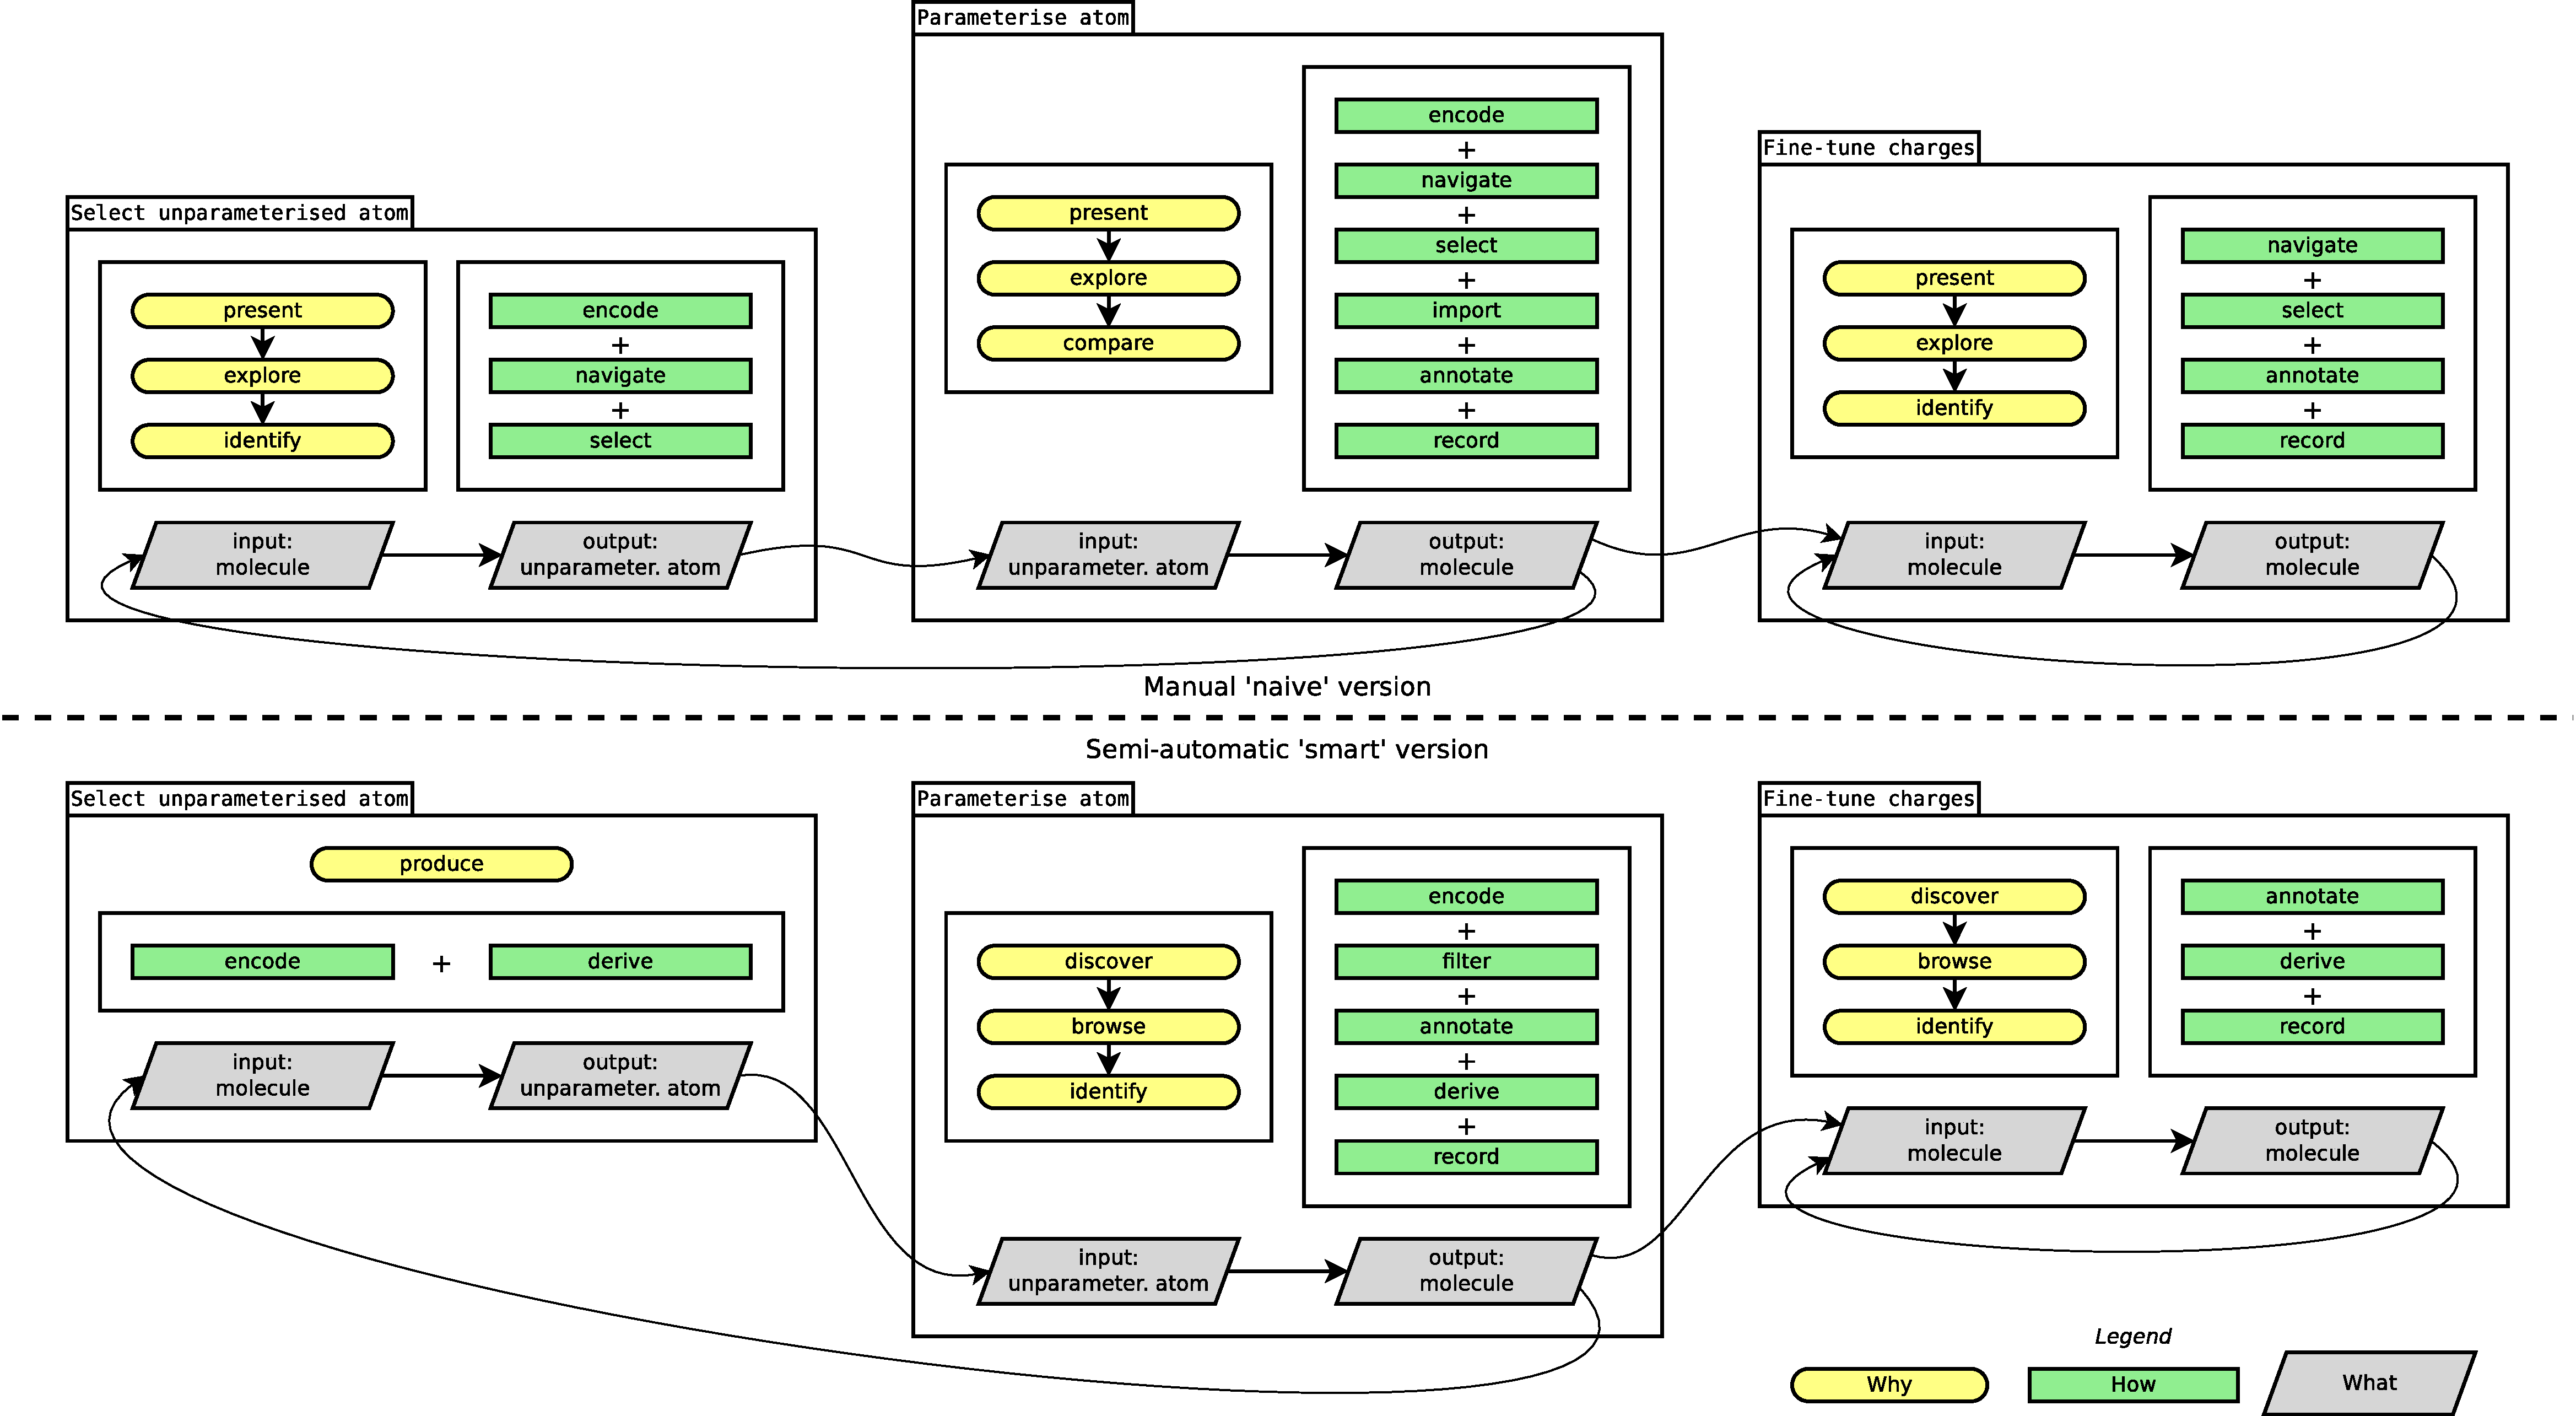
\includegraphics[width=\textwidth]{img/complete_typology.pdf}
\caption{Brehmer-Munzner Typologies of the two different interaction designs.}
\figlab{id_typologies}
\vspace{-2cm}
\end{center}
\end{figure}

The differences between the two versions are already very apparent in the second step of the parameterisation process, where atom selections are made. In the consuming version, the molecule needs to be presented to the user, after which he can navigate through it and identify an unparameterised atom by selecting it. The producing version of the system automatically makes atom selections. These only need to be shown to the user, and can be derived from the at that point visible molecule.

In the third step, the parameterisation of the atom, the differences are also clear. In the consuming version, found molecule fragments need to be presented in such way that they can be explored and compared by the user, after which he can select what he considers to be the best available match. The producing version, on the other hand, only requires the user to accept or reject a fragment. In other words, he needs to discover if a fragment is a good match by browsing through its details and identifying whether it is a good match or not.

Upon acceptance or selection of a fragment, it is possible that a charge conflict occurs (see also \secref{id_naive} and \secref{id_smart}). In the producing version, these conflicts are resolved automatically, but in the consuming one several solution methods need to be presented, from which the user has to select one. This leads to a great difference in the number of interaction methods that are used in the two versions, as finding the proper solution method can be quite complex.

This contrast in the number of different methods that is required to parameterise a molecule in the two versions is also apparent in the other differing steps. In every of those steps, the producing version requires less different methods than the consuming one. This means that, in the producing version, the user has easier access to the information, and can therefore make decisions quicker than in the other version. This does not necessarily mean that this version will take less time to use, as the methods may need to be used more often. What it does mean, however, is that it will be easier to learn how to use the producing version~\cite{sweller1994cognitive}~(see also \secref{id_learning}).

\chapter{Implementation}
\chlab{implementation}

A system for fragment-based molecule parameterisation has three distinct tasks: visualising a molecule, finding matching fragments for that molecule, and allowing for interaction with the molecule and its matching fragments. As these tasks can be performed in isolation, it has been decided to implement the molecule parameterisation tool as three separate systems.

The front-end of the system, where users will carry out the parameterisation process, will be called the Online tool for Fragment-based Molecule Parameterisation~(\oframp). This name will also be used to refer to the system as a whole, as it is the hart of the system and is dependent on the other systems. The molecule is also visualised in \oframp, but the for this purpose essential, calculations of atom positions are done in the Online tool for Atom Position Calculations~(\oapoc). Finally, finding matching fragments and sorting them based on relevance is done by the Online tool for Molecule Fragment Finding~(\omfraf).

The complete network diagram for the fragment-based molecule parameterisation system is shown in \figref{diagram}. It is clear that \oframp{} is the central system, but that the more computation-intensive tasks are carried out by \oapoc{} and \omfraf{}. The remainder of this chapter will discuss each of the systems in more detail.


\begin{sidewaysfigure}[p]
\begin{center}
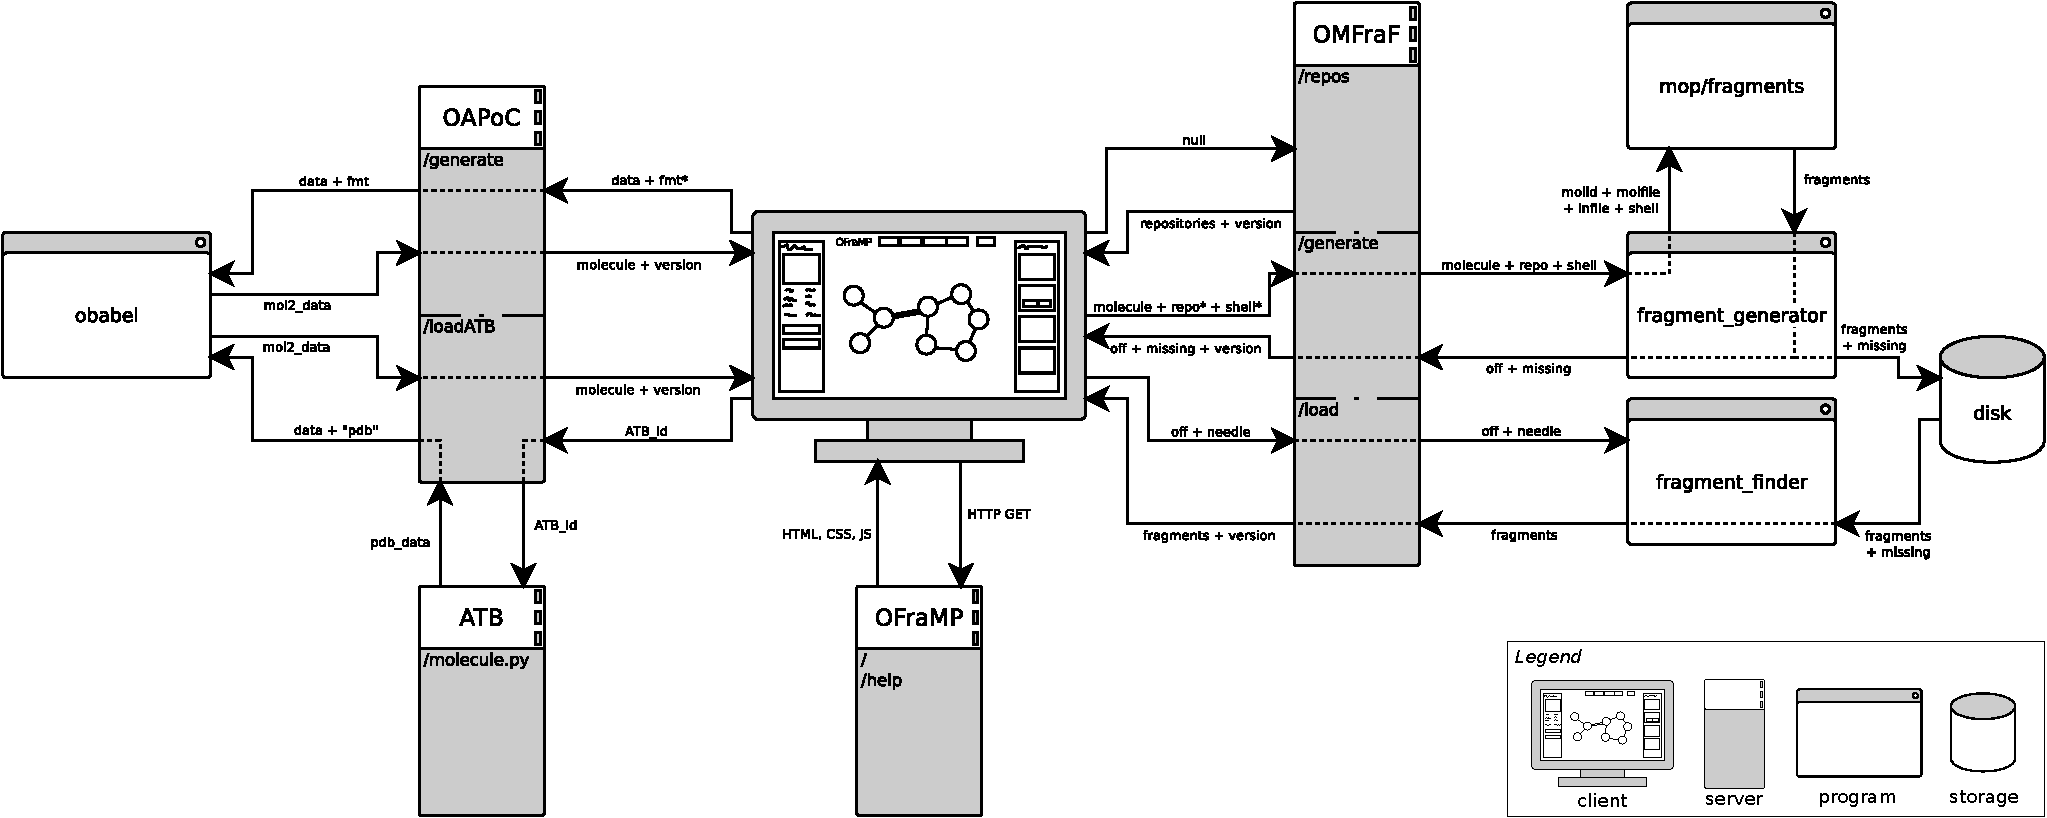
\includegraphics[width=\textwidth]{img/network_diagram.pdf}
\vspace{1em}
\caption{Network diagram of \oframp and its supporting systems.}
\figlab{diagram}
\end{center}
\end{sidewaysfigure}


\section[\oframp]{The Online tool for Fragment-based Molecule Parameterisation}
\oframp{} is the central part of the fragment-based molecule parameterisation system. It contains the user interface and connects with \oapoc{} and \omfraf{}. As discussed in \secref{platform}, it has been decided to implement the system as a web application. Following the current trend in web applications, \oframp{} has been implemented using the latest techniques from \verb|HTML5|, \verb|CSS3| and \verb|JavaScript|.

Using the latest web technologies allows for great cross-platform support. It allows the system to run on any desktop and laptop operating system, and creates the possibility of running it on a smartphone or tablet\footnote{This has not been a requirement for the project and has therefore not been tested extensively}, although the limited size of a smartphone screen can be problematic. Using the latest \verb|HTML5| technologies, however, also comes at a cost. Older browsers generally lack support, and will therefore not be able to run \oframp. Luckily, according to the latest browser statistics from StatCounter~\cite{statcounter2014statcounter}, almost 85\% of internet users uses a browser that has full support for these technologies. Thanks to the Internet Explorer canvas fallback \verb|excanvas|~\cite{arvidsson2009explorercanvas}, partial support can be provided for an additional 11\% of people, which results in a total support for 96\% of internet users.

\nlipsum

\begin{figure}[h!]
\begin{center}
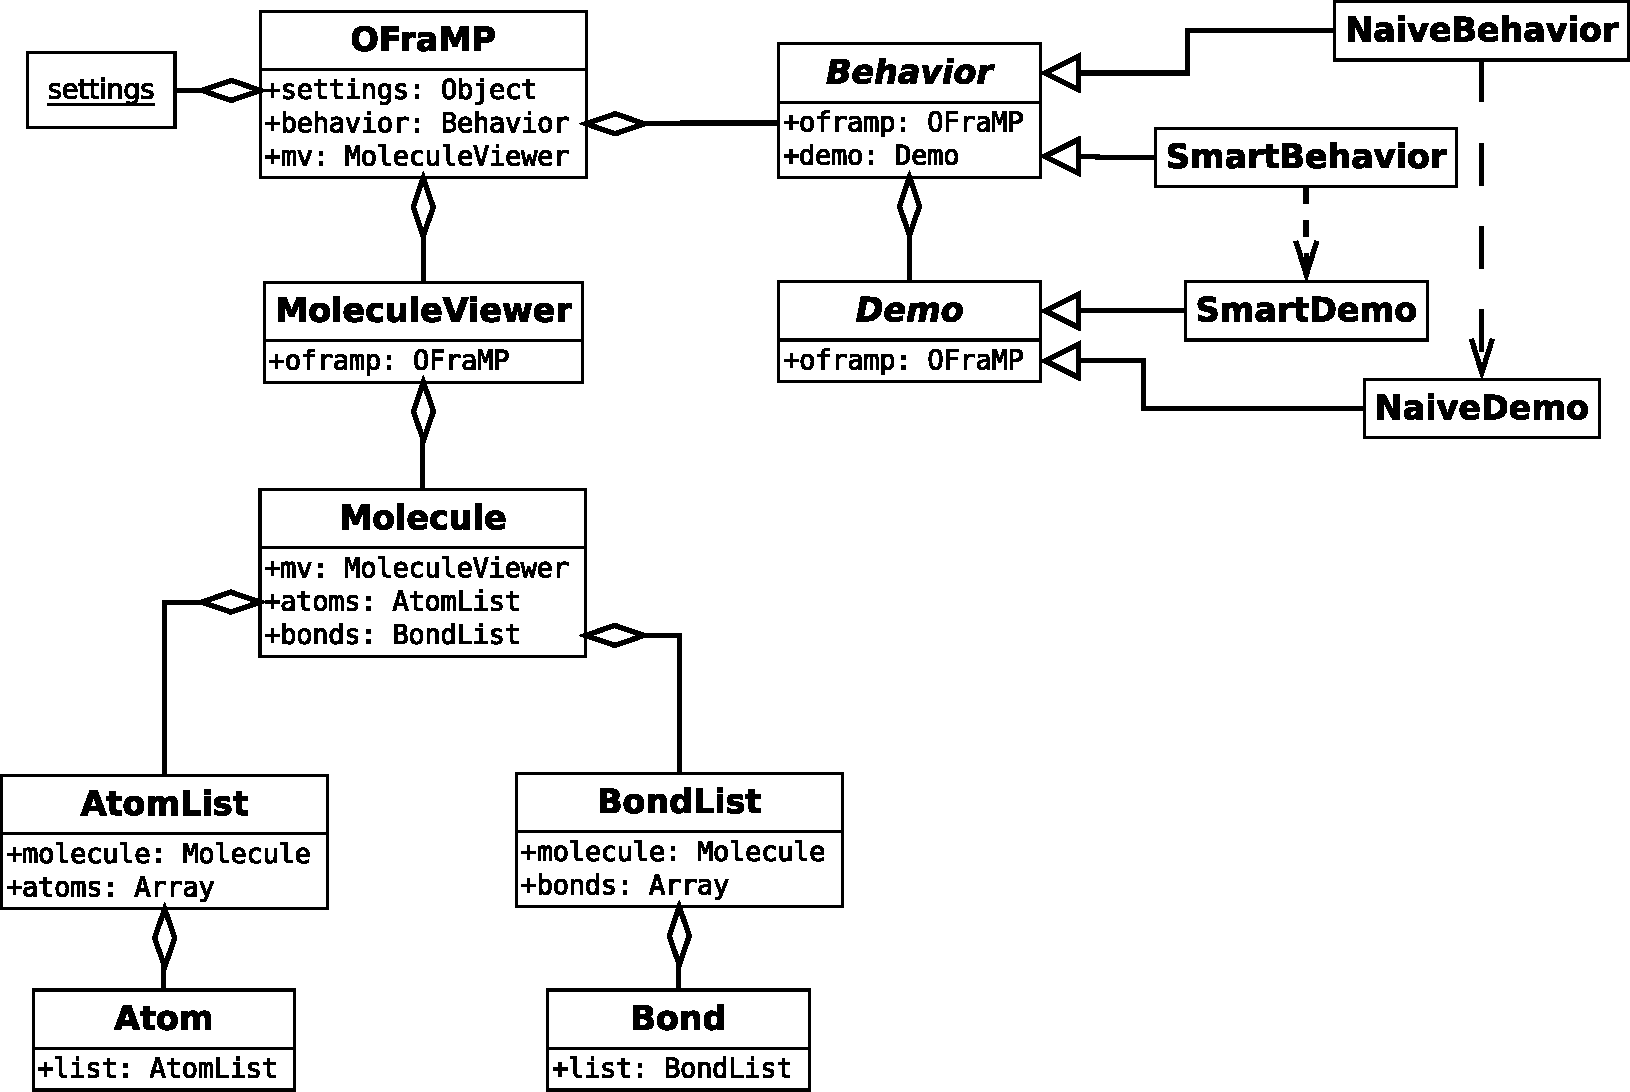
\includegraphics[width=\textwidth]{img/oframp_class.pdf}
\caption{Simplified class diagram of \oframp.}
\figlab{oframp_class}
\end{center}
\end{figure}

\subsection{Visualisation}
\nlipsum

\subsection{Interaction}
We use LGF files~\cite{dezso2011lemon}\ldots

\nlipsum


\section[\oapoc]{The Online tool for Atom Position Calculations}
\nlipsum

\subsection{obabel}
\nlipsum


\section[\omfraf]{The Online tool for Molecule Fragment Finding}
\nlipsum

\subsection{Generation}
\nlipsum

\subsubsection{mop/fragments}
\nlipsum

\subsection{Finding}
\nlipsum

\chapter{Evaluation}
\chlab{evaluation}

\begin{todo}
\item Completely redo chapter;
\item Move hypotheses to approach;
\item Move basic user studies description to approach;
\item Only discuss details of evaluation process here.
\end{todo}

In order to determine which of the two implementations of \oframp{} is the best, and to evaluate the project in general, the system will be subjected to a user study. This chapter will discuss the project's hypotheses~(\secref{hypotheses}) and the contents of the user studies, including the user tasks~(\secref{us_tasks}) and questionnaires~(\secref{us_questionnaires}). Finally, this chapter will discuss how the experiment outcomes should be analysed, and what certain outcomes should mean~(\secref{us_analysis}).


\section{Hypotheses}
\seclab{hypotheses}
According to Jonassen's dichotomy of problems~\cite{jonassen2000toward}~(see also \secref{id_learning}), fragment-based molecule parameterisation is an ill-structured problem. This means that the problem is quite complex and is therefore hard to solve. Due to this, users need to be ensured that there is a way to find a solution, or they will simply give up. This should be the case for both versions of the system, but is better facilitated by the naive version than the smart one. In the naive version, users will see that, by selecting an atom, it can easily be parameterised. He will know that, in order to complete the parameterisation, this process simply needs to be repeated for the remainder of the atoms.

The differences between the two implementations, as discussed in \secref{id_comparison}, combined with the motivations behind the two interaction designs~(see \secref{id_versions}), can lead to the conclusion that the smart version has great theoretical benefits in time consumption and user guidance, where the naive version should excel in user freedom. In the earlier mentioned study of Payne, Sycara, and Lewis~\cite{payne2000varying}, this was the same. They concluded that many users found that using the naive version was a tedious process that cost a lot of time. However, in some, more complex cases, they found that the system users find it really important to have full control of the system, and therefore preferred the naive interaction design. As fragment-based molecule parameterisation is an ill-structured, and therefore complex problem, the following hypothesis about the two versions of the interaction design can be formulated:
\begin{quote}
The `naive' interaction design is the best design for a tool that is used for fragment-based molecule parameterisation.
\end{quote}

On a more general level, both versions of the interaction design rely on the idea that fragment-based molecule parameterisation should be chemically correct. As this has not been proven yet, \oframp{} aims to help in determining if it is possible. Both versions of the system have been designed in such way that the user should be able to quickly parameterise a molecule, either by providing them with a clear overview of possibilities, or by limiting the user interaction to accepting and rejecting. Furthermore, as it has been proven that properly matching parts of molecules have the same atomic charges, the second - for both versions of \oframp{} essential - hypothesis is as follows:
\begin{quote}
It is possible to parameterise a molecule based on fragments of other molecules; both correctly and in a reasonable amount of time.
\end{quote}


\section{User studies}
To evaluate the hypotheses discussed in the previous section, both versions of the developed system will be subjected to a number of user studies. This will help to determine if the system works properly and whether it is really fit for the molecule parameterisation task. Unfortunately, not just anyone can be asked to test \oframp, as it is a system that is aimed to be used by experienced chemists who understand the details about molecule parameterisation. Luckily, project supervisors Klau and El-Kebir keep a close connection with a substantial group of chemistry researchers, creating the opportunity of asking them to participate in a user study. They were interested in the concept of fragment-based molecule parameterisation, and willing to test a system that does that.

\subsection{Use cases}
\seclab{us_tasks}
In the user studies, the participants will be split up in two groups, where each person is randomly assigned to a group and both groups are of equal size. This way, it is made sure that both groups are representative, which is essential for user studies~\cite{wohlin2003empirical}~(see also \secref{user_studies}). The groups will take part in an experiment that compares the two versions of the molecule parameterisation tool. Due to the limited number of test subjects, every participant will be asked to test both the naive and the smart version of \oframp. As the effects of the order in which two systems are evaluated are often remarkable, one group will start the evaluation with the naive version, followed by the smart version, where the other group will do this the other way around.

\begin{todo}
\item Explain why 2 molecules per version.
\end{todo}

For both versions of the tool, the experiment participants will be asked to complete the Demo mode first, such that they can get used to that version of the system. Next, they will be asked to parameterise a small, simple molecule, followed by a larger, more complex one. They are then asked to fill in a short questionnaire about that version of the system~(see \secref{us_questionnaires}), after which they are asked to switch to the other version of \oframp. When the steps for both versions have been completed, a final questionnaire, about \oframp{} in general, needs to be filled in. The complete set of instructions can be found in \appref{instructions}.

In order to be able to obtain results from the user studies, an extensive logging mechanism has been built into \oframp\footnote{This mechanism is only present in the special `experiment' version.}. It tries to log as much as it can; from browser details to system load times, and from mouse clicks to button presses. Every log message contains a time-stamp, such that the time difference between two log events can be calculated. They also include a message type, such that they can easily be filtered and counted. Finally, the resulting parameterisation is stored in the log as well, to be able to grade the user's performance.


\subsection{Questionnaires}
\seclab{us_questionnaires}
After completing their tasks on either of the two versions, the users will be asked to answer a number of questions about the tool. These will mainly be questions about how they like the design and if they can see themselves using it, but will also ask them for suggestions on things that can be improved or added. This way, their experiences can be used to further improve the system, and to make it into something they really like to use.

The questionnaire that test subjects will be asked to fill in will be based on the \verb|SUS| and \verb|UMUX-LITE| usability metrics~\cite{lewis2013umux}~(see also \secref{user_studies}). It will consist of the, for this tool, relevant questions from those metrics, followed by some questions about what they liked and disliked about the tool. To be certain that the questions are answered from the interaction design point of view, they will be asked from both the chemistry and interaction design perspectives. This gives the test subjects a place to put their comments on the chemical correctness, such that their feedback on the interaction design will truly concern the design. The complete set of questionnaire questions can be found in \appref{questionnaires}.

After testing both the naive and smart versions of \oframp, and assessing them with the previously discussed questionnaires, a few more, general questions will be asked. These questions are about what version the user liked best and why, if he wants to see any functionality added to the system, and leaves some room for additional comments. They will probably not provide new insights as to which version is liked better, as this can be inferred from the ratings obtained by the previous questionnaires, but they will help the further development of \oframp.

The questionnaires, just like the experiment, needed to be held online. Because of this, they have been implemented as web forms using (a minor extension of) the questionnaire language QL~\cite{erdweg2013state}. This allowed for easy definition of the form, without having to worry about validation or layout.

\subsection{Analysis}
\seclab{us_analysis}
The results from the log of the user studies combined with those obtained with the questionnaire should be able to give an answer on which of the two interaction designs is better. The version that gives good results in a short amount of time, and is also positively graded in the questionnaire, will be the better one. Furthermore, the timing and scoring results from the experiment alone will be able to answer the question if it is possible to do fragment-based molecule parameterisation at all. At least for one of the two versions both time consumption and parameterisation results should be reasonable.

In order to rate the user's parameterisation, the molecules that the user will be asked to parameterise should already have been parameterised using the conventional quantum mechanical calculations. This way, the user's results can be compared to the outcomes of the calculations to establish his rating. The smaller the difference between the two, the better the performance of the user will be graded.

There are two different ways of calculating this:
\begin{align*}
R &= |\Phi - C| & r &= \sum_{i = 1}^{n} |\delta_{i}|,
\end{align*}
\vspace{-1em}
\begin{align*}
\text{where} \quad \Phi &= \text{ATB total molecule charge},\\
C &= \text{\oframp{} total molecule charge},\\
n &= \text{total number of atoms in the molecule},\\
\delta_{i} &= \phi_{i} - c_{i},\\
\phi_{i} &= \text{ATB charge of the atom with index}~i,\\
c_{i} &= \text{\oframp{} charge of the atom with index}~i.
\end{align*}

First, it is interesting to know the difference in the total charge of the molecules, which is given by $R$. This is something that can be observed and minimised by the user, as he can see the totally assigned charge during the parameterisation process. It can therefore be used to see if the user is paying attention to that.

More important, but not less interesting, is the sum of the absolute differences between the two parameterisations, which is found by $r$. This will determine how good the results of \oframp{} really are, as it concerns the correctness of the individual atom charges.

Using the results obtained from the answers of the \verb|SUS| / \verb|UMUX| questionnaire, a final score can be calculated. This score is given by the following formula~\cite{sauro2011measuring}:
\[
s = 2.5 \times \sum_{i = 1}^{10} q_{i} - 1,
\]
where $q_{i}$ denotes the answer to question $i$.

In a study of over 500 outcomes of \verb|SUS| questionnaires, it has been found that the average system has a total score of $68$~\cite{sauro2011measuring}~(see also \secref{user_studies}). This means that, in order to be successful, at least one version of \oframp{} should score higher than that. Another study identified a way to translate \verb|SUS| scores to adjectives~\cite{bangor2009determining}. Systems with a \verb|SUS| score of below $20$ can be considered the `worst imaginable', a score of 48 to 65 is `OK', and 65 to 83 is `good'. The best version of the interaction design should therefore at least be rated as `good'.

\chapter{Results}
\chlab{results}

For the user studies, we invited a total of 16 chemistry researchers. They come from various institutes, but the majority works at VU University Amsterdam or the University of Queensland, Australia. Half of the invited received the instructions for the consuming-first version of the experiment, the other half was instructed to use the producing version first.

Out of all the invited people, 10 fully completed their tasks and submitted the results they obtained. 6 of them used the consuming version first, the other 4 started with the producing version. Unfortunately, it is impossible to tell how many people started the experiment, but did not finish it, as the log files were only uploaded to the server after completing a version's questionnaire. However, we observed that there were no people who only completed one of the two versions.

A lot of different types of data have been gathered. Graphical representations of most observations from the user action log can be found in \appref{graphs}. In that same chapter, one can find the outcomes of the \verb|SUS| and \verb|UMUX| questions that were asked in the questionnaire as well. \Appref{comments} contains all answers to the open questions, including general comments about the system, the preferred version and suggestions for improvement.

In this chapter, we present the important and most interesting results obtained from the user studies. Each result will shortly be discussed, and further analysed in \chref{discussion}. Some additional results are provided in \appref{results_extra}.


\section{Action log results}
From the logging system that was built into \oframp{} for the user studies, a wide range of information can be gathered, spanning from the load time and the number of clicks on atom 5 to the selected conflict solutions and resulting parameterisation. In this section, we present the most interesting results that can be retrieved from the action log.

\subsection{Time required}
\seclab{res_time}
First of all, it is interesting to see in which version users spent the most time to fully parameterise the molecules. \Figref{graph_time_1} shows the total time that was required for both the first and second set of molecules, in both the consuming and producing version of \oframp. What can be seen here is that, for both the first and second set of molecules, users needed more time to complete the parameterisation using the consuming version. Users who started with the consuming version used the most time overall, with a median total time of around 300 seconds. Those same users spent the least time on the producing version, where the median time value is around 100 seconds. At around 200 and 150 seconds, one can find the median times required by the users who did the consuming version second and the producing version first respectively.

\begin{figure}
\center
\includegraphics[width=.6\textwidth]{img/graphs/1a_02.pdf}
\caption{Total parameterisation time for the two versions in the two orders.}
\figlab{graph_time_1}
\end{figure}

The total time used to parameterise the first and second sets of molecules can be used to determine which version of \oframp{} is the most time-consuming. However, as both sets of molecules have slightly varying molecule sizes, it may be more interesting to look at the average time that was required per atom. This can be seen in \figref{graph_time_2}.

\begin{figure}
\center
\includegraphics[width=.6\textwidth]{img/graphs/1a_03.pdf}
\caption{Average time per atom for the two versions in the two orders.}
\figlab{graph_time_2}
\end{figure}

What is interesting to see here, is the fact that, where in the total parameterisation time, the group that did the producing version second was done the fastest, its members have spent the most time on average per atom. When taking a closer look at \figref{graph_time_3} and \figref{graph_time_4}, which show the average time per atom required for all molecules separately, this difference appears to be caused completely by the excessive amount of time users spent on parameterising molecule 13913 in the producing version. This is the first molecule users got to parameterise after they completed the consuming version. Even more interesting to see is the fact that most users spent more time on this 11-atom molecule than they did on the larger 77-atom molecule 17738.

\begin{figure}
\centering
\begin{subfigure}[t]{0.48\textwidth}
\centering
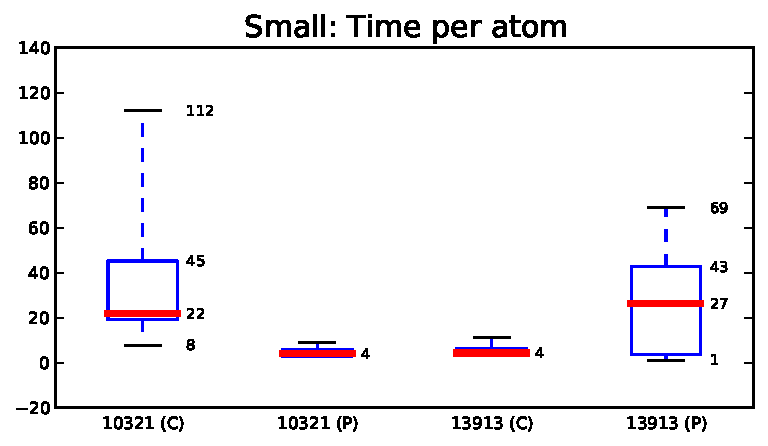
\includegraphics[width=\textwidth]{img/graphs/1c_03.pdf}
\caption{Smaller molecules.}
\figlab{graph_time_3}
\end{subfigure}%
~
\begin{subfigure}[t]{0.48\textwidth}
\centering
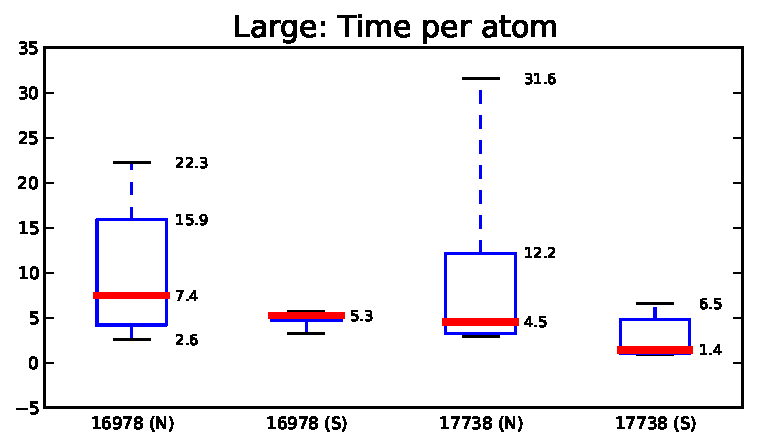
\includegraphics[width=\textwidth]{img/graphs/1d_03.pdf}
\caption{Larger molecules.}
\figlab{graph_time_4}
\end{subfigure}
\caption{Average time per atom for all molecules in the two orders.}
\figlab{graph_time_34}
\end{figure}

It is hard to say what exactly is causing this difference. It is possible that, after using the consuming version, it is hard to get used to the producing version, which is way more restrictive as to what a user can do. This difference is not present when switching from the producing to the consuming version, which can either mean that this switch is easier to make, or that there must be a different cause of the large time difference.

Another possible explanation for the large increase in time required for parameterising molecule 13913 is that there may not be really good matching fragments, enforcing the user to browse through many of them before being able to select what they consider to be the best one. This is better facilitated by the consuming version of the tool, and can potentially have the extreme effects that are observed here.

% Apart from molecule 13913, \figref{graph_time_34} shows that finishing a parameterisation using the consuming version of \oframp{} requires more time than using the producing one. It is also clear that the time required is much more constant, and, with an overall average of around 7 seconds per atom, overall still the fastest, compared to 10 seconds for the consuming version.


\subsection{Parameterisation rating}
\seclab{res_rating}

\begin{figure}
\center
\includegraphics[width=.6\textwidth]{img/graphs/1a_00.pdf}
\caption{Total charge difference for the two versions in the two orders.}
\figlab{graph_rating_1}
\end{figure}

Not only the time required by the parameterisation tool can be used to assess the two interaction designs, the quality of the result is also of great importance. As discussed in \secref{ev_analysis}, there are two ways of calculating this quality rating. First, the total difference between the charge found by the user and the charge present in the ATB is shown in \figref{graph_rating_1}. As this difference can easily be observed and corrected by the user, it would be expected that it would be relatively close to 0. This, however, turns out not to be the case. Especially in the producing version of \oframp, the charge difference can get quite high, and is greater than the charge difference for the consuming version in any case.

What is also interesting to note here is the fact that, for both the consuming and the producing version of \oframp, the total charge difference is higher for the second set of molecules. This may indicate that these molecules are harder to parameterise, or that there are no good matching fragments available for those molecules. However, it may also indicate that users were starting to lose their concentration, or were confused due to the switch from one version to another.

Whereas the difference in the total molecule charge can mainly be used to assess user performance, the correctness of the parameterisation can better be measured using the per-atom charge differences. \Figref{graph_rating_2} shows these differences for the first and second set of molecules, both for the consuming and producing version of \oframp. As can be seen in that graph, charge differences are, again, smaller for the consuming version than they are for the producing version.

\begin{figure}
\center
\includegraphics[width=.6\textwidth]{img/graphs/1a_01.pdf}
\caption{Average charge difference per atom for the two versions in the two orders.}
\figlab{graph_rating_2}
\end{figure}

In contrast to the total charge differences though, the average charge differences for the second set of molecules are smaller than those for the first set. This suggests the opposite of what was concluded from \figref{graph_rating_1}: the second set of molecules may be easier to parameterise, or there may be better matching fragments available. This suggestion is more probable, as, for the total charge difference, a negative offset between two atom charges can be compensated by a positive offset in two others. This is not the case for the per-atom difference.

\begin{figure}
\centering
\begin{subfigure}[t]{0.48\textwidth}
\centering
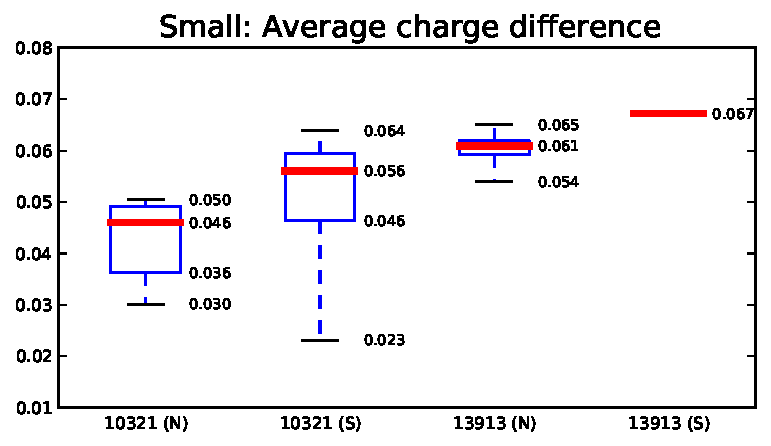
\includegraphics[width=\textwidth]{img/graphs/1c_01.pdf}
\caption{Smaller molecules.}
\figlab{graph_rating_3}
\end{subfigure}%
~
\begin{subfigure}[t]{0.48\textwidth}
\centering
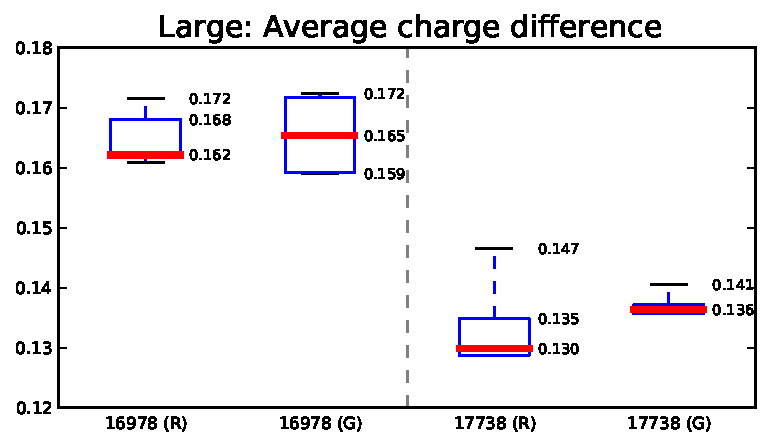
\includegraphics[width=\textwidth]{img/graphs/1d_01.pdf}
\caption{Larger molecules.}
\figlab{graph_rating_4}
\end{subfigure}
\caption{Average charge difference per atom for all molecules in the two orders.}
\figlab{graph_rating_34}
\end{figure}

As can be seen in \figref{graph_rating_34}, the consuming version of \oframp{} scores better for all individual molecules. What can also be seen there is the fact that, even on average, the charge differences are bigger for the larger molecules than for the smaller ones. Unfortunately, there is no obvious explanation for this. Probably, larger fragments are used for the larger molecules. When one of those fragments is bad, it quickly adds up to the atom charge difference. On the other hand, it is also possible that users felt more comfortable selecting small fragments, which are generally worse matches than the large ones, due to less atoms matching between the two molecules.

\subsection{Other results}
\seclab{res_other}

\begin{figure}
\center
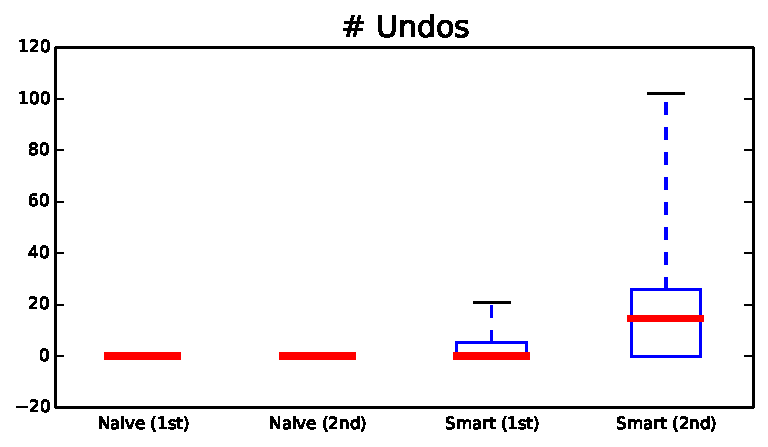
\includegraphics[width=.6\textwidth]{img/graphs/1a_10.pdf}
\caption{Number of undo actions for the two versions in the two orders.}
\figlab{graph_undo}
\end{figure}

Besides the time required to complete the parameterisation and its rating, some other interesting things were observed in the user studies. First of all, there appears to be a great correlation between the version of \oframp{} that is used and the amount of actions a user needs to undo, as we can see in \figref{graph_undo}. Where, in the consuming version, users practically do not undo any action, there are extreme cases where a user undid over a hundred actions in the producing version. This difference can be explained by the fact that users of the producing version have to undo accidentally rejected fragments, or may use a combination of reject and undo actions to compare various fragments.

\begin{figure}
\center
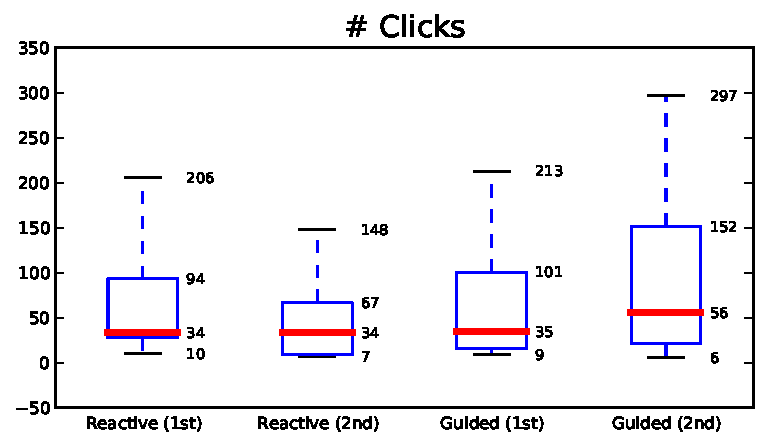
\includegraphics[width=.6\textwidth]{img/graphs/1a_04.pdf}
\caption{Total number of clicks for the two versions in the two orders.}
\figlab{graph_clicks}
\end{figure}

As can be seen in \figref{graph_clicks}, a few more clicks are required to complete a parameterisation in the producing version of the tool, than there are in the consuming version. Nevertheless, the medians are not too far apart, so it is not really possible to draw any conclusions from this. It is interesting to see, however, that even though the producing version of \oframp{} requires less user interaction, is does not require less, and possibly even more clicks to complete a parameterisation.

\Figref{graph_help} shows that not many users had to consult the help pages during the parameterisation process. Furthermore, no users checked the help pages in their second version of the system. This can mean that either they did not know there were different versions of the help pages, or they did not need it any more. The fact that most users did not go to the help pages at all suggests that the tool is intuitive to use, and that taking the demo provides enough information to be able to use \oframp.

\begin{figure}
\center
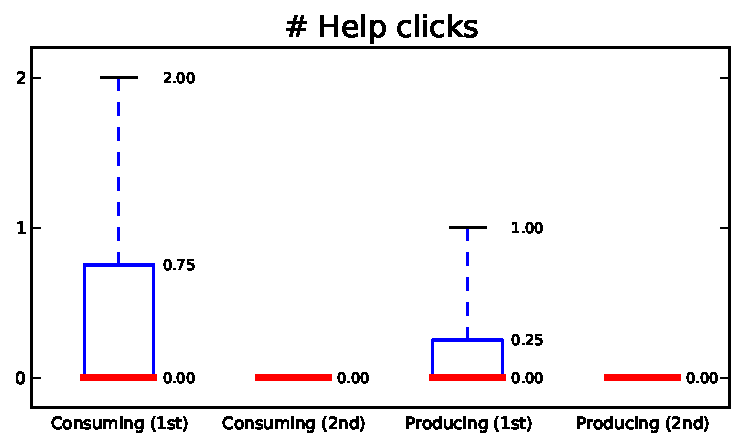
\includegraphics[width=.6\textwidth]{img/graphs/1b_01.pdf}
\caption{Total number of clicks on the help button for the two versions in the two orders.}
\figlab{graph_help}
\end{figure}

There are also a few things users did not do at all. They were not required or instructed to use every aspect of \oframp, but it was expected that they would at least try some of the more advanced features. First, none of the users used any of the available keyboard shortcuts. Although all actions for which a keyboard shortcut exists can also be completed using a single mouse click, it was expected that some users would find it beneficial to use keyboard shortcuts for some actions.

Furthermore, and more surprisingly, none of the users manually edited a single atom charge. Again, they were not specifically instructed to do so, but they were made aware of the possibility of doing this, and instructed to make the parameterisation as good as possible. Possibly, they just did not feel the need of it, or thought their parameterisation was perfect the way it was. However, some users commented they were unable to locate the position of the charge edit fields, suggesting otherwise~(see also \secref{res_comments}).



\section{Questionnaire outcomes}
Besides the log files from the users parameterising a few molecules, some more information can be gathered from the questionnaire users were asked to fill in. This includes the results of the combined \verb|SUS| / \verb|UMUX| questionnaire, their preference verdict on the two versions, and other comments about the system. We will discuss all of these in the next sections.

\subsection{\texttt{SUS} / \texttt{UMUX} results}
\seclab{res_sus}
The total \verb|SUS| score of the consuming and producing versions of the system is shown in \figref{graph_sus_1}. As can be seen here, the consuming version, with a median rating of $76$, scores better than the producing version, which has a median rating of only $61$. This means that the consuming version scores above the average \verb|SUS| score of 68~\cite{sauro2011measuring}, where the producing version scores below that. In the adjective rating scale, the consuming version is `good', but the producing version still scores `OK'~\cite{bangor2009determining}~(see also \secref{ev_analysis}).

\begin{figure}
\center
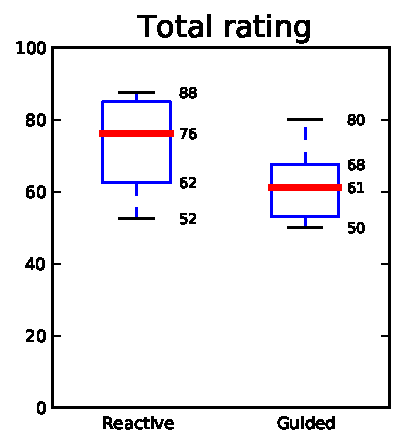
\includegraphics[width=.32\textwidth]{img/graphs/4a_10.pdf}
\caption{\texttt{SUS} score of the two versions.}
\figlab{graph_sus_1}
\end{figure}

\Figref{graph_sus_2}, where the ratings are shown separately for the two different orders in which the users used the two versions of \oframp, shows a slightly different situation. First of all, it appears that the group that did the consuming version first was less positive in general. With a median grade of only 62, the consuming version scores below average and is rated as just `OK'. Although it is still rated higher than the producing version, with outliers to very high ratings, the difference in the medians is very small and not really significant.

\begin{figure}
\center
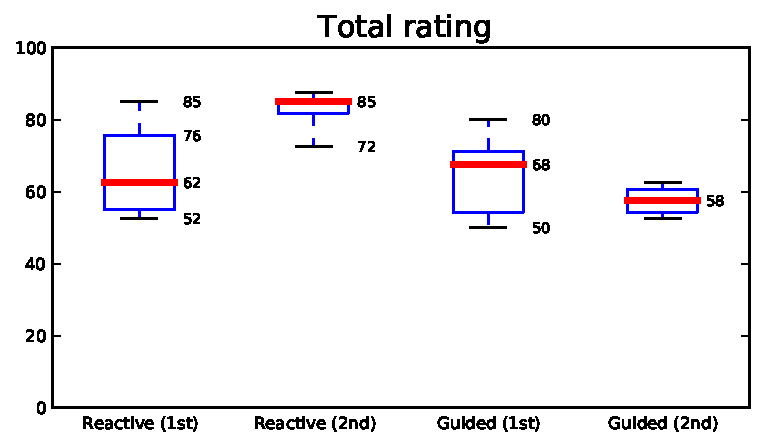
\includegraphics[width=.6\textwidth]{img/graphs/4b_10.pdf}
\caption{\texttt{SUS} score of the two versions in the two orders.}
\figlab{graph_sus_2}
\end{figure}

For the other group of users, the opposite is true. They already awarded the producing version with the average grade of $68$, and later rewarded the consuming version with a rating of $85$, which translates to `excellent' on the adjective scale. This large difference can possibly be explained by the users preferring the consuming version over the producing one and therefore, consciously or unconsciously, giving higher grades to the consuming version. The lower, but still `OK' grading of the producing version in the other group can then be explained by the users still liking the producing version, and therefore willing to grade it sufficiently.

The most extremely rated \verb|SUS| questions are shown in \figref{graph_sus_345}. \Figref{graph_sus_3} shows the lowest scoring point for both the consuming and the producing versions of \oframp, being the answer to the first \verb|SUS| statement: ``I think that I would like to use this system frequently''. Whereas, for the consuming version, most people are neutral, with some agreeing or even fully agreeing with the statement, the median answer in the producing version was a disagree. This is an important result, as users not liking to use a system frequently is, of course, a bad sign.

\begin{figure}
\centering
\begin{subfigure}[t]{0.32\textwidth}
\centering
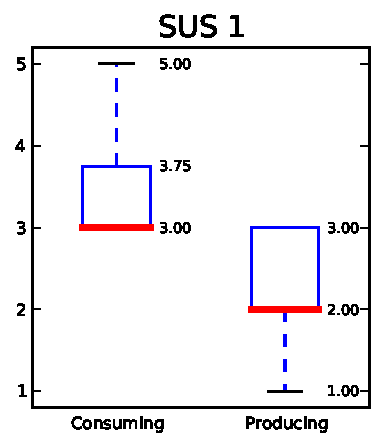
\includegraphics[width=\textwidth]{img/graphs/4a_00.pdf}
\caption{Rating of \texttt{SUS1}.}
\figlab{graph_sus_3}
\end{subfigure}%
~
\begin{subfigure}[t]{0.32\textwidth}
\centering
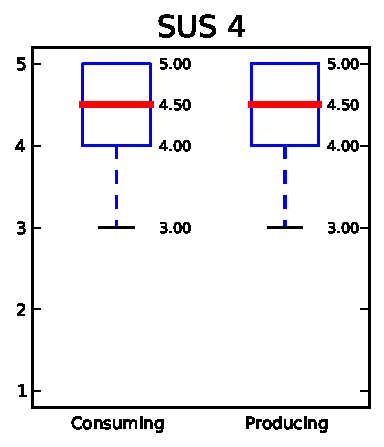
\includegraphics[width=\textwidth]{img/graphs/4a_03.pdf}
\caption{Rating of \texttt{SUS4}.}
\figlab{graph_sus_4}
\end{subfigure}%
~
\begin{subfigure}[t]{0.32\textwidth}
\centering
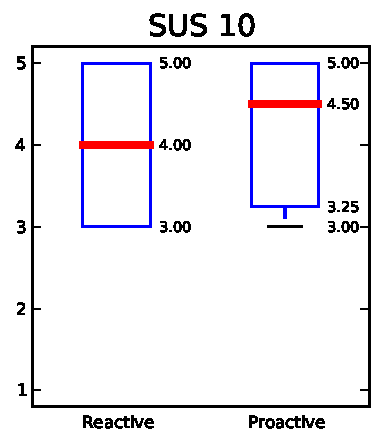
\includegraphics[width=\textwidth]{img/graphs/4a_09.pdf}
\caption{Rating of \texttt{SUS10}.}
\figlab{graph_sus_5}
\end{subfigure}
\caption{Selected ratings for the two versions of \oframp.}
\figlab{graph_sus_345}
\end{figure}

The fourth \verb|SUS| question was the highest rated for both the consuming and producing versions of the system~(see \figref{graph_sus_4}), although the tenth question is rated equally high in the producing version. \verb|SUS4| states: ``I found the various functions in the system were well integrated''. As there is no difference in the rating of the two versions, no conclusions can be drawn for this, other than the fact that both interaction designs are well-integrated in general.

Finally, as mentioned before, the tenth \verb|SUS| question is one of the highest rated for the producing version. Furthermore, this is the only statement for which the producing version actually scores higher than the consuming one. As the tenth statement is ``I think the system meets up with its requirements'', it is quite interesting that the producing version scores higher here. Probably, the test participants considered the required time to complete the parameterisation an important requirement. As seen before, the producing version requires the least time, which may explain the difference here.


\subsection{Preference}
\seclab{res_preference}
The general questionnaire users were asked to submit after they were completely done started off with the question which version of the system they preferred. All participants actually preferred the consuming version, no matter whether they had to use that first or last. Most users commented that they felt they had more control over the parameterisation process in that version, which they thought they really needed. Furthermore, they preferred seeing a list of possible matches over the accept/reject system.

Additionally, some users commented that the consuming version allowed for easier comparison of fragments, compared to having to make a combination of rejects and undos in the producing version. One user even commented this made the parameterisation process a lot quicker, though the timing results discussed before tell a different story. This means that the consuming version \emph{feels} faster, and suggests that the parameterisation process using the producing version may be considered to be tedious.

\subsection{Comments}
\seclab{res_comments}
Following the \verb|SUS| and \verb|UMUX| questions, users were asked to answer a few open questions and had room for some comments. In the next sections, we will discuss these comments for both versions of \oframp{} and the suggestions they had for improving the tool. As we have not observe any significant difference between the comments of the people for the different orders in which they used the system, no distinction will be made between those comments.

\subsubsection{Consuming version}
For the consuming version of the system, users were very positive about the user interaction. They noted that the interface and layout were very clear and nicely designed, and also gave a nice representation of molecules and fragments. The interface was found to be very responsive and easy to use and learn, thanks to the demo mode, the extensive help pages, and the fact that the system was intuitive to use in general. Finally, the right information was noted to come up exactly when needed.

Users were also enthusiastic about the chemical concepts behind \oframp. They liked the idea of fragment-based molecule parameterisation in general, and specifically the fact that this allows them to iteratively assign charges to a molecule. Furthermore, they found that there was a good variety of fragments available to complete the parameterisation. However, the ordering of these fragments could use some work, as the highest rated ones are in fact rarely the best available matches. It was also commented that using a shell around the atoms to find matching fragments may not be the best way to find good matches, as this will not detect all atomic properties.

There were some critical notes about the user interface as well. Some users found the `finished' popup confusing and annoying. A few users commented that it was hard to keep track of the total molecule charge, and that this should be visible at all times. Others had trouble finding out how to scroll the list of found fragments, presumably due to the alternatively styled scrollbars.

There were also some disagreements between different users. Where some really liked the colour coding of the atoms, and especially the indication of the conflicting fragments, others found the used colours confusing and suggested using different ones. It was also noted that it made no real sense for users to manually decide which (group of) atoms needed to be selected, while others highly valued this.

Finally, many users noted that they would like to be able to manually alter or insert charges for certain atoms. As was already suspected from the analysis of the action logs, users did not find the charge edit functionality in the selection details window. A user also commented that he would like to be able to see what fragments have been  used to parameterise an atom. This is available in the same place where the charges can be edited, and further confirms the idea that it has to be positioned in a more prominent spot, or indicated in a better way.


\subsubsection{Producing version}
In their comments about the producing version of \oframp, users were, again, quite positive about the interface. They noted it to be clear and running smooth, and liked the visualisation of the molecule. Additionally, they found the tool extremely easy to learn, and mentioned it helped them to parameterise a molecule very quickly. It was mentioned again that fragment-based molecule parameterisation is a good concept to speed up molecule parameterisation. Finally, the ability to view the original molecule was found to be truly valuable.

Despite all the positive feedback, all users encountered one major problem: they were not able to easily compare different fragments. This either resulted in them having to go through some sort of reject/undo loop, or made them select a fragment before they were confident that it was the best available. Furthermore, they noted that taking the average of the conflicting atom charges is not always a good solution, and they needed to be able to decide how the conflict should be solved. Some users also commented that the automatic atom selection was too arbitrary, and needed to be more intelligent.

Most of the shortcomings of the consuming version were also mentioned here. Again, many noted that they needed to have an easy way to keep track of the total molecule charge. Some found the `finished' popup obstructive, and it was mentioned once more that making matches based on a shell around the target atoms may not be the best approach.

\subsubsection{Suggestions for improvement}
\seclab{res_suggestions}
Many users had some ideas for further improving the value of \oframp. The following list contains the most mentioned and feasible ones, ordered on descending number of mentions.
\begin{enumerate}
\item Continuously show the total molecule charge:\\
Even though the molecule charge can be viewed in the selection details window, this window is not opened at all times. Additionally, the effect of selecting a proposed fragment on the total charge can be shown with it;
\item Ability to manually add/edit charges:\\
As discussed before, many users wanted to see this feature added, even though it is already present. Additionally though, they commented that they would like to be able to assign a charge to a group of atoms, and have this automatically distributed over the group;
\item Combine the auto-select system with the fragment list:\\
Some users noted they did not want to manually select atoms all the time, and liked the automatic selection system from the producing version. As this was lacking the overview of fragments, they wanted to combine it with the list of fragments from the consuming version to make the ultimate parameterisation system;
\item Show the confidence score of fragments:\\
It was noted a few times that this would help in finding the best available fragment;
\item Indicate identical sections in the atom that is being parameterised:\\
In some molecules, sections of atoms occur multiple times. For these sections, the charges are generally equal. It would therefore be useful if these sections would be highlighted and will probably be useful to copy the charges automatically;
\item Remember the position of the popup:\\
As the popup location is reset every time, users have to move it to the side every time they want to compare an original molecule to the input molecule. Some therefore consider it better to remember the location the popup was dragged to once it is reopened;
\item Colour coding of atom types:\\
It has been noted to be common practice in chemistry applications to colour code atoms based on their type. Some users would like to see that in \oframp{} as well.
\end{enumerate}

\chapter{Discussion}
\chlab{discussion}

From the results obtained in the user studies, it can be decided which version of \oframp{} is the best for the task of fragment-based molecule parameterisation. What version that is will be argued in this chapter, along with a description of how it can be improved in the future. Additionally, some threats to the validity of the experiment outcomes will be discussed.


\section{The best version}
There are several factors that can help to determine which interaction design for \oframp{} is the best. First, the time required to complete a parameterisation can be considered. As discussed in \secref{res_time}, the smart version requires the least time per atom, and will therefore be the fastest to completely parameterise a molecule. With a total median time of under five minutes for parameterising all four molecules in the user study, it can also be considered to be fast in general. Time-wise, the smart version is therefore the best.

Second, one can look at the correctness of the resulting parameterisations of the different versions. The results presented in \secref{res_rating} show that the naive version has the lowest overall charge difference for both the first and second set of molecules. Furthermore, it has a lower average atom charge difference for every parameterised molecule as well, with average differences of $0.054$ for the smaller molecules, and $0.146$ for the bigger ones. This means that, result-wise, the naive version is the best.

The final information that can be gathered from the user action log is the number of actions that needed to be undone, and the total number of clicks that needed to be made to complete the parameterisations. As was described in \secref{res_other}, the naive version required almost no undo commands, while the smart version required the use of many. Furthermore, the total number of clicks was also smaller for the naive version, making this the better version in those two aspects as well.

Besides the action logs, the \verb|SUS| ratings of the two versions of the system can be used to decide which one is best. As discussed in \secref{res_sus}, the naive version scored higher than or equal to the smart version for all but one statement. Additionally, with a total \verb|SUS| score of $76$, it not only had a higher score than the smart variant, but was also graded above average, and `good'.

The comments that user studies participants made on the smart version were less positive than those made on the naive version. This also showed in their preference verdict, where all participants voted for the naive version, rather than the smart variant~(see \secref{res_preference}). Most of them commented they strongly preferred that version.

Combining all of this data, it is clear that the naive interaction design is the better of the two. It gives better results, and is found to be better fit for molecule parameterisation than the smart design. Even though it takes slightly more time to complete a parameterisation in that version, it still is reasonably fast. However, it may not be considered the perfect interaction design yet. Many suggestions on how it could be improved have been made~(see \secref{res_suggestions}), resulting in some future work which will be discussed later in this chapter.


\section{Threats to validity}
As in every research project, there are always a few threats to the validity of its outcomes. For the conclusions on the best interaction design for \oframp, this is no different. Most important here is the limited number of participants in the user studies. Due to the limited amount of people currently involved in manual molecule parameterisation, and the limited amount of time in which they had to complete the experiment~(one week), only 10 people were able to partake. However, it has been shown that a sample size of only 10 people leads to a correct \verb|SUS| conclusion $80\%$ of the time~\cite{tullis2004comparison}.

This limited amount of experiment participants also lead to the decision that every user would have to test both versions of the system. While this is not a bad thing in general, it would have been preferred to do a double-blind test to make sure users were not primed by the first version they used. It has been attempted to mitigate this risk by dividing the participants over two groups, where both would use the systems in a different order, but this does not rule out any effect it may have had on the results.

The fact that users had to test both versions of the system unfortunately also doubled the time they needed to complete the experiment. Even though all parameterisations were completed in under 10 minutes on average, users also had to complete two different demo modes and fill in three questionnaires. This brings the total time for the average user to around 45 minutes, where, in extreme cases, users took far over an hour from loading the first version to submitting the final questionnaire. This may potentially have lead to loss of concentration, and might have incited users to take shortcuts in the parameterisation process, although this has not explicitly been observed.

By organising the user studies over the internet, there has been no control of the environment in which the participants performed the experiment. Although the users were instructed to make a large time slot available for it, and asked to try to focus on it as much as they could, it may be possible that they got interrupted at certain points, or used the system in a busy environment. This, unfortunately, is one of the insuperable side-effects of conducting an on-line user study.

Another possible threat to the validity of the results is the choice of molecules for the user study. For the experiment, four molecules (two small, two large) were randomly selected from the \verb|ATB|. It is unknown whether these were good example molecules or not, as they may have some special properties. furthermore, similar molecules may not exist at all.

Additionally, as commented by many users, the fragment finding system is not perfect yet. It does sometimes find matches that do not make a lot of sense from a chemistry perspective, and the rating system needs to be improved such that the best matches will in fact also be the highest rated. Even though the development of the fragment finding system was outside of the scope of this project, it can still have had some influence on the outcomes.

In order to find the best interaction design for a fragment-based molecule parameterisation system, two different designs have been implemented and compared. Although there was a strong preference for the naive version, it may be the case that a third, completely different system would be even better. However, even though the users had many suggestions on how the system could be improved further, none of these suggestions was really ground-breaking from the interaction design point of view. This does not rule out the possibility of the existence of an even better version, but does reduce the chances for it.

Finally, an unfortunate implementation/design error in the system that stored the user comments lead to the loss of the comments of two users. Although their \verb|SUS| ratings did not really deviate from the others, it may be the case that they made some different comments, or actually picked the smart version as their preferred one. Sadly, there is no way to recover these comments, but the similarity of the \verb|SUS| results suggests that there was no big difference of these users' opinion.


\section{Future work}
Thanks to the large amount of suggestions for improvement~(see \secref{res_suggestions}), \oframp{} can be developed further to enhance the user experience. First of all, as this was the most requested feature, the total molecule charge should be shown at a place where it is always visible, along with the charge effect of the previewed fragment, when there is one.

Second, some thought should be put into the location of the atom charge edit fields. As many users commented they wanted to see this added, it needs to be positioned at a more prominent position. Alternatively, manually editing atom charges may be added to the demo, or more emphasis could be put on the current location.

The third most suggested alternation is the possibility to automatically select atoms in the naive version. As some users also commented they really liked the fact that they had full control over which part of the molecule was parameterised at which time, a toggleable auto-select system should be built into the tool. This will satisfy the needs of both groups of users.

Additionally, the remainder of the suggestions listed in \secref{res_suggestions} should be added to \oframp{} as well. They have all been examined, and it is believed that they can improve the user experience, without hurting it in any way.

As soon as the previously listed modifications have been implemented, a new, small user study should be conducted to confirm that these changes truly increase the value of \oframp. Additional user studies will also help to support the earlier made claims about the fragment-based molecule parameterisation system in general. With a larger sample size, the obtained results will have a higher confidence ratio, reducing the chances for false conclusions.

Finally, although that is technically outside the scope of this project, the fragment finding and rating system needs to be improved. Even when the interface for the fragment-based molecule parameterisation system would be perfect, the system would be useless if the found fragments are of a low quality. Luckily, the fragments are already acceptable, and there are ideas on how the matching system can be improved further. Once it has been updated, it needs to be reintegrated with \oframp, but, unless the protocol changes, that should be trivial.
 % With future work section
\chapter{Conclusion}
\chlab{conclusion}

In an attempt to speed up the molecule parameterisation process, we have developed a new approach that uses fragments of parameterised molecules to find the charges of individual atoms in an unparameterised molecule. We implemented this new approach in a system called the Online tool for Fragment-based Molecule Parameterisation~(\oframp). Two different versions of it were designed, called \IDa\ and \IDb, and have been compared by performing a user study.

From the user study, we have concluded that the \IDb\ interaction design allows users to be done quicker, while the \IDa\ version yields more accurate results. The users showed a strong preference for the \IDa\ design. They liked the overview they had of the matching fragments, and felt like they were more in control than in the \IDb\ version. This has turned out to be an important aspect, and is required to make a good parameterisation of a molecule.

In addition to this, users rated the \IDa\ version better than the \IDb\ one. With a \verb|SUS| score of 76, it is even rated higher than the average system, and good in general. For the complex task of fragment-based molecule parameterisation, we consider user satisfaction and result correctness to be the most valuable aspects of the system. Therefore, the \IDa\ interaction design has been selected as the overall better of the two.

More in general, most of the common features of the two versions were appreciated as well. First, the graphical design of the application was found to be very clean and clear, and noted to look professional. Second, users were enthusiastic about the way in which the molecules are visualised, the ability to move them around and scale them, and the responsiveness of the visualisation. The selection details window was found to be very useful, and the demo mode helped them to quickly learn how to use the system. Finally, although not everyone used it, the help pages were highly appreciated for their extensive descriptions of every aspect of \oframp.

There were, of course, also some negative comments. Often, the found fragments were not ordered correctly, and the best available match rarely ended up on top of the list. Furthermore, there were even situations in which barely matching fragments were rated to be very good. Although the development of the fragment finding system was not a part of this project, it needs to be improved further in order for \oframp{} to be able to attain its full potential.

Additionally, many suggestions for improvements and additions to the system have been provided. They span from the addition of an auto-select mode for atoms, to the modification of certain atom colours. The suggestions need to be evaluated in order to determine which of them are useful, and which are not. Implementing the right suggestions will definitely help to improve the quality of \oframp\ even further.

Once all alterations to the system have been made, we believe that it will become a tool using which a parameterisation can be obtained that can compete with one obtained using the conventional quantum-mechanical calculations. Furthermore, chemists will be able to fully parameterise a molecule using \oframp{} in less time than when using the conventional methods.

All these findings support our hypotheses, which were posed in \secref{ra_hypotheses}. The \IDb\ interaction design we presented turned out to take up less time than the \IDa\ one. This version in turn, delivered more accurate results, was rated higher by its users, and is therefore considered the overall better version. Using \oframp, it should definitely be possible to create a molecule parameterisation of equal quality to the calculated ones, in less time.

Finally, from a general interaction design perspective, the findings of this project suggest that for complex, unexplored tasks like fragment-based molecule parameterisation, the best results can be obtained using a design that gives the user full control over the system. Without a validated set of rules on how exactly the task needs to be performed, automating certain parts of the system might overlook complex aspects of the task and therefore result in bad output. For this type of tasks, one should rather implement a non-automated version of the system first, in order to establish a set of rules for the automation. Later, the possibility of automating (parts of) the process using those rules can be examined.


\cleardoublepage
\phantomsection
\addcontentsline{toc}{chapter}{Bibliography}
\bibliographystyle{abbrv-rt}
\bibliography{references}
\chaptermark{Bibliography}

\appendix
\chapter{Additional literature}
\chlab{relwork_extra}

\wip

\section{Interaction design}
Besides trying to optimise the preparation steps for molecule simulations, the main challenge of this thesis project is to come up with a good interaction design for a tool that does that. In the interaction design area, Donald Norman is a respected and often cited author. He feels that technology can only live up to its full potential by, first of all, supporting human tasks, while making the supporting technology as transparent as possible~\cite{norman2002design}. This can be achieved by making the tools easy to use, easy to learn and easy to understand. Designing for this purpose is called user-centred design.

%

Despite the fact that the importance of design has been long known, many software products are still poorly designed. In an attempt to overcome this, an approach called human-centred design (HCD) has been developed~\cite{norman2005human}. However, even though the needs of the user play a central role here, many companies following the HCD principles still develop complex and confusing products. The systems are often superb at the level of the static, individual display, but fail to support the sequential requirements of the underlying tasks and activities. Therefore, a new approach is needed that does not put the user in a central role, but rather does so with the activity that needs to be performed. In this Activity-Centred Design~(ACD) method, it is sometimes necessary to ignore a user's requests, as they might compromise the task that has to be carried out.

This, however, does not mean that the application user's needs should be completely ignored. On the contrary, it is really important that the user's characteristics are understood and used in the design of an application~\cite{badre2002shaping}. Also, a good analysis of the context is needed to make the right design decisions. If one ignores the user characteristics and context of an application, the application is  likely to fail, as the context in which the application is developed will almost always differ from the context in which it will be used.

%

\subsection{Learning}
\seclab{id_learning}
In order to determine what makes a good interaction design, it needs to be known how people learn new things and how our problem solving system works. There are two main learning mechanisms: schema acquisition, where knowledge of subject matter is organized in schemas that determine how new information is dealt with, and the transfer of learned procedures from controlled to automatic processing~\cite{sweller1994cognitive}. Well learned material can be processed automatically, without much effort, while new or less familiar information needs to be processed in a controlled fashion. This means that, when learning something new, one can only use that knowledge by devoting considerable cognitive effort to it. After getting more familiar with the task, the skill may become automatic. Only then can intellectual performance attain its full potential.

In order to facilitate learning, the process of schema acquisition needs to be triggered and supported. Trying to teach by only providing examples will eventually even have the opposite effect. The learner will then be able to execute the task under the conditions that are equal to those in which he learned the skills, but will fail to do so in other cases. In order to overcome this, teaching should be done using goal-free problems. These problems focus on achieving various problem states and the steps on how to get there, which is exactly how schema acquisition works.

How easy it is to learn something new is highly dependent on the level of interactivity between the different elements of a task. If there is no interaction between two elements, they can be learned in isolation, requiring less cognitive load than when they have to be learned simultaneously. However, making something easy to learn is not as simple as reducing the element interactivity, as it is dependent on the knowledge of the individual what constitutes an element. For the more experienced, an element may be a whole chunk of the information, while for the rest it may just be an atomic part of the information. Luckily, it is only hard to learn something new when both the intrinsic and extraneous cognitive loads are high. When there is only one high load, the lack of the other compensates for this.

There are two types of problems: well-structured problems and ill-structured problems. In a well-structured problem, the initial state is well-defined, the goal state is known, and there is a limited set of logical operations to solve the problem~\cite{jonassen2000toward}. If either of these is missing, the problem is classified as being ill-structured. Ill-structured problems are generally more complex than well-structured problems, and are therefore often harder to solve.

Besides the complexity, there are also many individual differences that determine how easy it is to solve a problem. First of all, when a person is familiar with the domain of a problem, it will be easier to solve for him than it will be for someone with less domain knowledge. Second, more analytical thinkers are often good problem solvers. They must believe that there will be a way to solve the problem, especially when the problem is ill-structured, as they might otherwise just give up before finding a solution. It also helps when someone has a certain affection with the problem. He will then be more likely to try and find the solution. If, however, one has certain beliefs or attitudes about a problem and its solution, he might be a less effective problem solver due to over-relying on that solution. Finally, every problem is different and requires different skills to solve. It can be easier to solve the problem for someone who is familiar with the problem type, but one may never forget that every problem requires a different way of learning.

%

\subsection{Interaction design principles}
Thimbleby, on the other hand, \emph{does} relate his principles to technology~\cite{thimbleby2007press}:
\begin{itemize}[noitemsep,topsep=0pt,parsep=0pt,partopsep=0pt]
\item Use good algorithms for better user interfaces: interactive devices are designed to solve problems in a structured way, which is exactly what a good algorithm does;
\item Use simple, explicit interaction frameworks: those provide clear interaction structures, which allow for reliable feature integration, checking, analysis, fault identification, and error fixing;
\item Interrelate all interaction programming: all aspects of the design should come out of the same specification;
\item Define properties and analyse designs for them.
\end{itemize}
A more extensive list is provided by Blair-Early and Zender~\cite{blair2008user}:
\begin{itemize}[noitemsep,topsep=0pt,parsep=0pt,partopsep=0pt]
\item Obvious start: design an obvious starting point;
\item Clear reverse: design an obvious exit or stop;
\item Consistent logic: design an internally consistent logic for content, actions, and effects (the most important consistency is that with user expectations);
\item Observe conventions: identify and consider the impact of familiar interface conventions;
\item Feedback: design tangible responses to apt user actions;
\item Landmarks: design landmarks as a reference for context;
\item Proximity: design interface elements in consistent proximity to their content objects and to each other;
\item Adaptation: design an interface that adapts or is adapted to use;
\item Help: as necessary, provide a readily accessible overall mechanism for assistance;
\item Interface is content: design interface elements that minimise interface and maximise content.
\end{itemize}

The above lists of principles are all quite different, but all consider automation of certain processes. The next section will discuss this in more detail.

%

\subsection{Automation}
Automation is often said to be causing problems and to increase the chances for human error when failures occur. Norman proposes in~\cite{norman1990problem} that this is not the cause of automation itself, but rather of the automated systems' lack of appropriate feedback when humans need to take over control. In regular conditions and some predefined exceptional situations, automated systems are perfectly able to operate. It is in those other abnormal situations that automated systems often fail; both in executing their task and alerting the user that something unusual is happening. In order to overcome this, automated systems should be designed while keeping in mind that errors will occur. An appropriate feedback system needs to be present that allows for human intervention when needed.

An often used, but wrong way of alerting a system's user that something is wrong, is the use of alarms for every component of the system~\cite{norman1990problem}. In exceptional situations, multiple components will often fail at the same time. When all of these would sound an alarm, the user could get confused and will not know what component requires immediate attention and what can wait. Rather than this, systems should continually inform the user about their state, such that he can detect exceptional situations and act upon them. Still, this information should be non-intrusive and presented in a natural way, such that man and machine can jointly solve the problem at hand.

%

\section{Molecule software}

\subsection{Molecule visualisation}
Molecule visualisation is generally done using either two-dimensional schematic views, or three-dimensional structure models. Which of these forms is best depends on the application for which the visualisation needs to be used. In cases where correct perception of the molecule structure including bond angles, bond lengths, and atom sizes is needed, 3D representations need to be used. A study on Slovenian primary and secondary schools has shown that, for understanding chemical concepts, 3D models are highly beneficial if they can be interacted with~\cite{ferk2003students}. However, as they convey more information than the 2D representations, it does take more time for the students to understand the 3D models. Furthermore, as the structures often have to be converted to a 2D form which the students can draw in their notebooks, transition rules need to be taught, which increases the steepness of the learning curve even further.

%

When a molecule in a textual format that lacks positional information needs to be visualised, its atoms' positions need to be calculated. Starting from the 1970s, algorithms for schematically displaying molecules in 2D have been developed. Dittmar, Mockus and Couvreur created one of the first programs that converted a connection table to a structural molecule diagram~\cite{dittmar1977algorithmic}. Back in the day, computing power was limited, which meant that advanced operations to eliminate overlap in the visualisation needed to be limited. Nevertheless, computing the diagrams still took over three minutes for an average sized molecule. Since then, advances in computer hardware and algorithm improvements have made it possible to speed up the structural diagram generation to times of under a second~\cite{fricker2004automated}. The improvements of computer hardware also allowed for better overlap prevention in the diagrams, leading to much cleaner visualisations~\cite{clark2006structure}. However, overlap is still not completely eliminated, so there is a need for further improvements in these algorithms.

%

A different study on the use of computer programs in biology unveiled some more requirements~\cite{taylor2013interface}. First of all, it is highly beneficial to have different visual representations of the molecule, or to at least be able to modify the visualisation parameters at runtime. This allows the application user to fully tailor the visualisation to his needs. Second, as visualisations are usually only there to make a certain task easier, they should not get in the way of that task. Finally, even though the main goal of the visualisation is often to answer questions, it should also have the potential of posing new ones. A good visualisation shows things that were previously unknown, which have the potential of raising new questions.

%

\section{User studies}
%% Not all this has been left out...
In Software Engineering, an often used method to evaluate a project is performing a user study. In general, user studies can be assigned to one of the following categories: experiments, case studies, surveys, and post-mortem analyses~\cite{wohlin2003empirical}. In all of these types of studies, it is important to have a representative group of test subjects. These should preferably be picked at random from the population of application users.

In the first type of user studies, the experiment, two (or more) different configurations of the examined tool are compared by examining the effects the configuration has on the tool's output~\cite{wohlin2003empirical}. It is important to define exactly what one wants to validate~\cite{stein2009assessing}. This should preferably be something that can easily be observed (e.g. `time required' or `number of clicks', but not `comprehensibility'). Furthermore, it is important that all different configurations are semantically equivalent (i.e. doing the same thing), have an equal degree of compression (i.e. contain the same information) and are formatted into their cleanest and clearest extent.

Before starting an experiment, it is very important to make sure the subjects are committed to the tasks they need to perform. Otherwise, the experiment will not properly reflect the production environment. Furthermore, the experiment should be well-prepared, as start-up problems might negatively impact the subject's opinion otherwise.

Another type of user studies is the survey. In a survey, it is easy to test a large number of variables, but one should be careful not to test too many, as this will make the analysis infeasible~\cite{wohlin2003empirical}. In order to collect questionnaire information in a structured way, its questions should follow some natural flow that embodies all aspects of a user's experience~\cite{tuch2013analyzing}. This encourages them to report their detailed experiences, as this is less demanding than answering one big open question. Furthermore, it also reduces the chances of subjects failing to report certain things, simply because they forgot about them.

A few predefined surveys are available for usability testing, including \verb|SUS|~(System Usability Scale)~\cite{brooke2013sus} and \verb|UMUX|~(Usability Metric for User Experience)~\cite{lewis2013umux}. \verb|SUS| consists of ten items, each of which should be graded on a scale of 1 (strongly disagree) to 5 (strongly agree). It has been extensively tested and turns out to have a reliability score of 0.96. \verb|UMUX| is a shorter questionnaire, consisting of four questions, with a reliability score of 0.86. However, its even shorter brother, \verb|UMUX-LITE|, consisting of only two questions, has been shown to provide results of the same reliability. It is believed that when a system is subjected to both \verb|SUS| and \verb|UMUX-LITE|, one can get very reliable results on the usability of that system.

On a final note about surveys, the fact that they are often straightforward makes them perfectly suitable for being held over the internet. It has been shown that the results of online surveys do not significantly differ from their offline counterparts~\cite{komarov2013crowdsourcing}. However, face-to-face surveys are still the only way that allows both the interviewer and the test subject to immediately ask and answer questions~\cite{wohlin2003empirical}. Nevertheless, the effects of this are considered minimal and can often be mitigated by asking the test subject if he has any questions in the questionnaire.

Before analysing the data obtained by a user study, it is important to validate it~\cite{wohlin2003empirical}. All the obtained results should be complete and correctly documented. Furthermore, extreme outliers should be identified dealt with. What should happen exactly depends on the situation, but in most cases it is best to leave out the extreme results~\cite{komarov2013crowdsourcing}. Finally, it is very important to provide a grade of validity along with the conclusions of the user studies. This grade depends on, for instance, the number of test subjects, their representativeness or the distribution of the results.




\chapter[Additional implementation]{Additional implementation details}
\chlab{implementation_extra}

Whereas the earlier implementation chapter~(\chref{implementation}) discussed \oframp{} at a higher, not too technical level, we will discuss its technical details in this chapter. Many descriptions rely on understanding of the network diagram that was presented in that chapter, in \figref{network_diagram} on \figpageref{network_diagram}.



\section[\oframp]{The Online tool for Fragment-based Molecule Parameterisation}
As we can see in \figref{oframp_class}, a \verb|JavaScript| \verb|OFraMP| instance forms the heart of \oframp. This instance contains a \verb|settings| object containing the complete configuration for the system, a \verb|Behavior| implementation, and a \verb|MoleculeViewer|. We will discuss these types, and all others in the class diagram, in the next sections.

\begin{figure}
\center
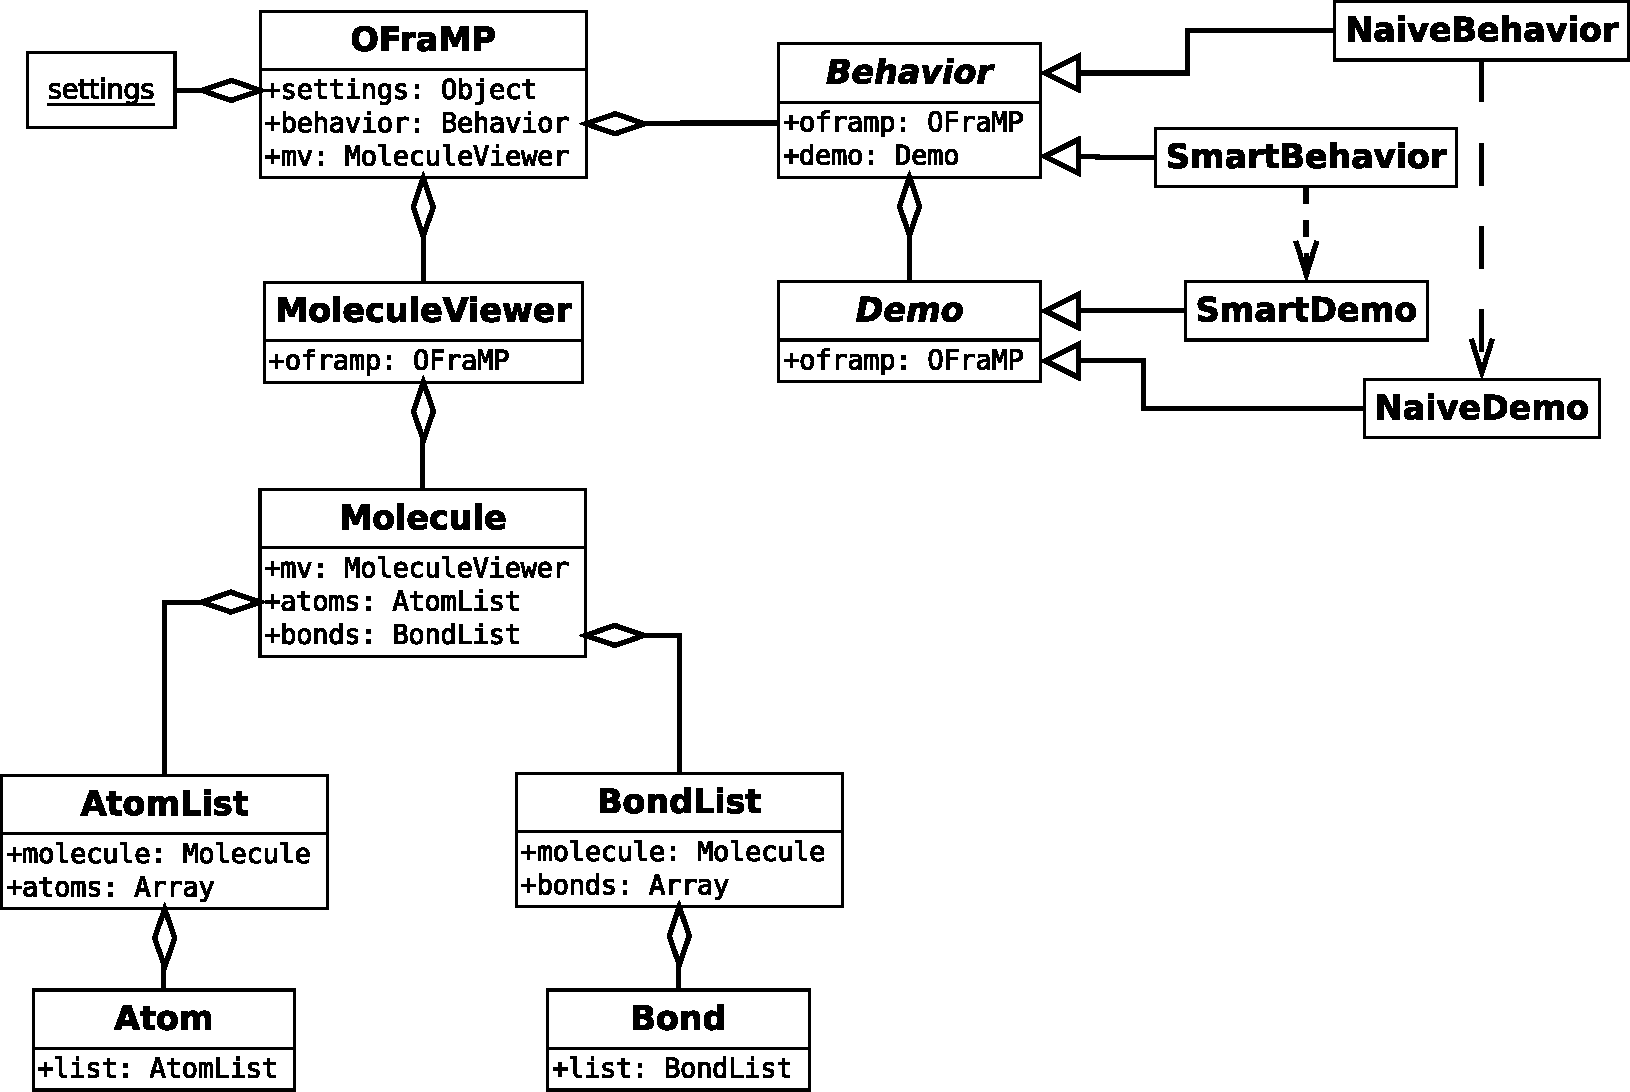
\includegraphics[width=\textwidth]{img/oframp_class.pdf}
\caption{Simplified class diagram of \oframp. The \IDa\ and \IDb\ versions were initially called naive and smart respectively, hence their occurrence in the class names.}
\figlab{oframp_class}
\end{figure}


\subsection{Visualisation}
Once a molecule data string has been entered into the system, the positions of its atoms and the connections between them are retrieved from \oapoc~(see \secref{impl2_oapoc}). This data is then transformed to a \verb|JavaScript| \verb|Molecule| instance, as can be seen in \figref{oframp_class}. \verb|Molecule| instances can be visualised using a \verb|MoleculeViewer|, which will draw the molecule onto an \verb|HTML| \verb|canvas|.

\subsubsection{Deoverlapping}
As discussed in \secref{rw2_visualisation} and~\cite{clark2006structure}, overlap in atoms and bonds still occurs in modern molecule visualisation software. In the case of \oframp, where the atoms have a relatively large radius to make room for displaying the charge, chances are even higher. To temper the effects of this, a simple deoverlap algorithm has been implemented.

\Figref{impl_deoverlap} shows the three different types of deoverlapping that \oframp{} can perform. Here, the light blue line indicates a vector that is used to determine if there is any overlap, the red line indicates the overlapping part, and the green arrow~(of equal length to the red line) shows where the atom centre should be moved to in order to resolve the overlap.

By default, for performance reasons, only the deoverlapping of atoms is enabled. This is the easiest to detect and solve, but also the most important one. Atoms that overlap almost entirely might not be spotted by the user, and atom types and charges may become hidden 
\begin{figure}
\center
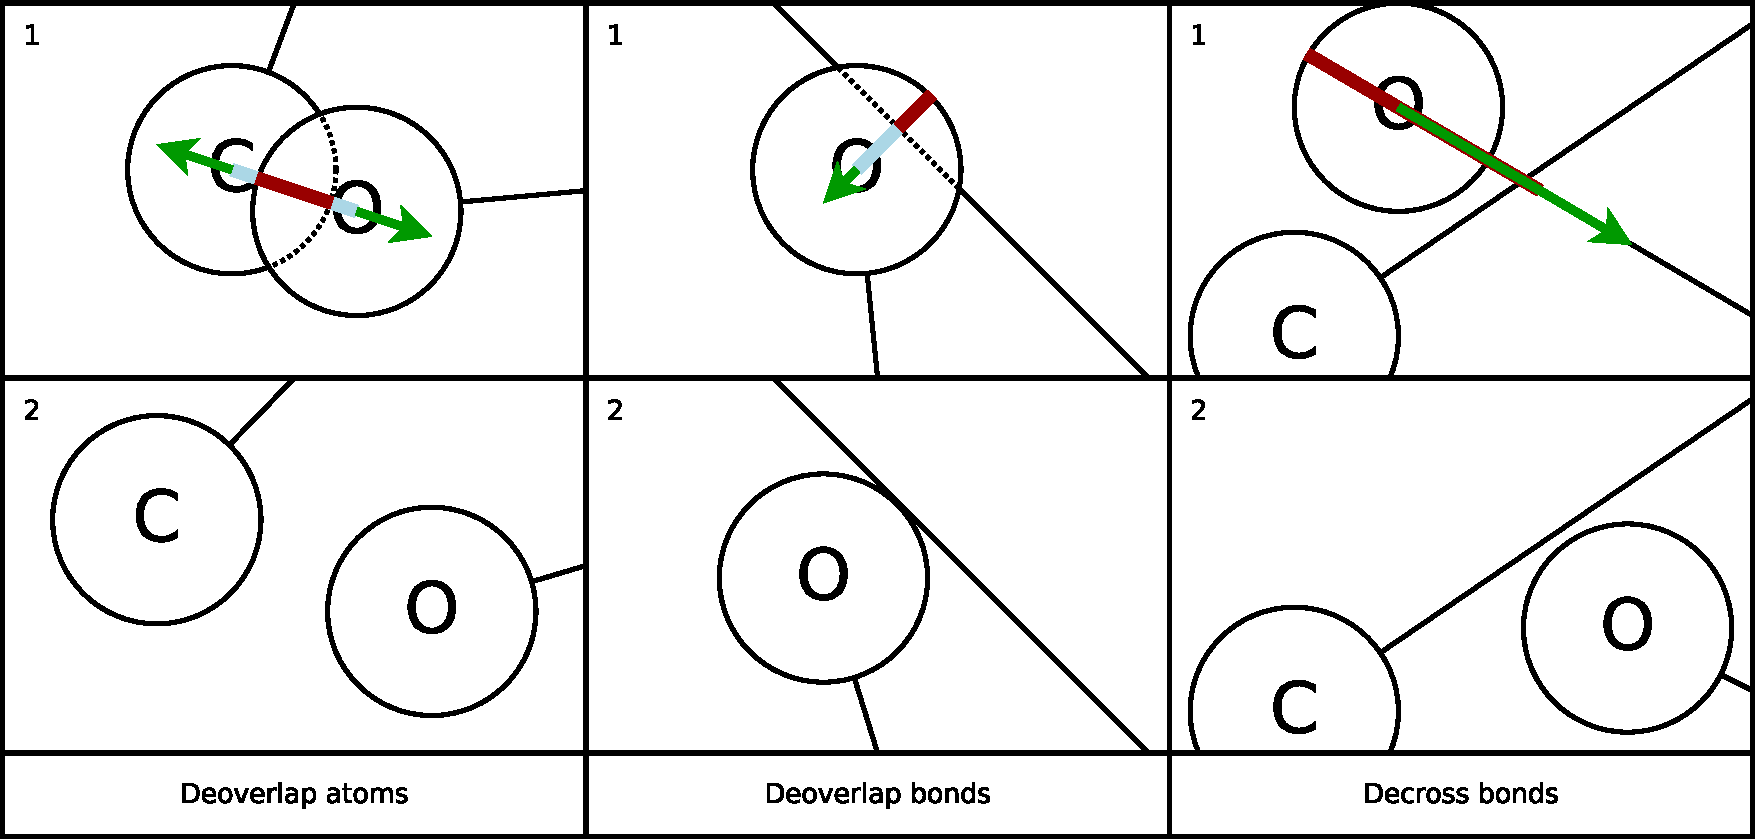
\includegraphics[width=\textwidth]{img/deoverlap.pdf}
\caption{Concepts of deoverlap.}
\figlab{impl_deoverlap}
\end{figure}due to another atom lying on top of them. As can be seen in \figref{impl_deoverlap}, this type of deoverlap works by calculating the distance between the two atom centres and subtracting the atom radius from that twice~(once for each atom). If this distance is smaller than $0$, both atom centres will be moved along the line that connects the two for a distance that is equal to the overlap distance. This ensures that the atoms will no longer overlap, and even creates some room between them.

In order to solve atoms overlapping bonds, the perpendicular distance from the atom centre to the bond needs to be calculated. When this distance is smaller than the atom radius, the atom needs to be moved along the perpendicular for a distance that is equal to the overlap distance. This will put the atom right next to the bond.

The third and final type of deoverlapping, the so-called decrossing of bonds, is also the hardest one. First, it needs to be determined if the two bonds intersect each other. When that is the case, the intersection point needs to be found. The overlap distance here is equal to the distance from the atom centre to the intersection point, plus the radius of the atom. One of the atoms then needs to be moved along its bond for a distance that is equal to the overlap distance, in order to solve the crossing bonds.

Unfortunately, solving one occurrence of overlap could result in overlap occurring in a different place, as moving an atom could potentially move it on top of another. Therefore, the deoverlap process will need to repeat itself to solve all overlap in the molecule. However, it is possible that the solution of one overlap occurrence is the exact opposite of another, which means that, after two iterations, the situation will be exactly the same as it was initially. In order to prevent the deoverlap process from going into an endless loop, a time limit~(set to half a second by default) has been built in, after which the deoverlapping will stop.


\subsection{Parameterisation}
In order to find a good interaction design for \oframp, two different interaction designs of it have been made. In order to allow for easy implementation of these different versions, a \verb|Behavior| interface\footnote{\texttt{JavaScript}, as of \texttt{ECMAScript} 5, does not have real interfaces, but the \texttt{Behavior} object acts as one.} has been created~(see \figref{oframp_class}). When a new behaviour for the system is designed, implementing this is as easy as making an implementation of that interface. As each interaction design also needs to have its own demo mode, the \verb|Demo| has been implemented as an interface as well. Implementing a demo mode for a different interaction design is therefore just as easy as creating the new \verb|Behavior| implementation itself.


\subsection{Downloading results}
\seclab{impl_downloading}
When the user feels he is completely done, or at any other point in the process, he can download the resulting parameterisation of the molecule by clicking the `Download' button at the top of the page. This will give him the result in the \verb|LEMON Graph File|~(LGF) format~\cite{dezso2011lemon}. We decided to use this format for the output file, as it is used by, among others, the fragment finding system~(see \secref{impl2_omfraf}), and because it is a flexible format that can easily be generated. The output file will contain all atoms' element types, \verb|IACM| number, and charge, as well as all bonds between the atoms.


\subsection{Modifying visualisation parameters}
In order to allow for modification of visualisation parameters at runtime, a slightly modified version of the \verb|JavaScript| library \verb|dat-gui|~\cite{data2011dat} has been used. Using the extension we made, this library can automatically generate a user interface from a \verb|JSON| object that contains the settings. Additionally, it can be provided with an object that contains various settings for the interface itself, such as which widget to use, and change event handlers.


\subsection{Saving progress}
Throughout the whole process, the user has the ability to download a checkpoint file that contains all his progress up to that point. This so called \oframp\ State Storage~(OSS) file can be loaded back into the system later, such that it functions as some sort of save file. In addition to the typical save file contents, OSS files also store the action history. This means that there is absolutely no penalty to stopping parameterisation at some point and continuing on it some time later. It allows users to work on a molecule for a bit, even if they do not have enough time to fully complete it.



\section[\oapoc]{The Online tool for Atom Position Calculations}
\seclab{impl2_oapoc}
Provided with a molecule data string~(MDS) and optionally a format specification for that string, \oapoc{} will provide the detailed molecule data~(e.g. atoms, atom positions, bonds) that is encoded in the MDS. Internally, \oapoc{} uses the \verb|Open Babel| program \verb|obabel| to convert the MDS to the \verb|Mol2| format, which we have chosen as it can easily be parsed and contains information on atom positions and bonds. Furthermore, it does not leave out the $H$ atoms, which some other formats do. For some applications this is fine, but for \oframp{} it is required to have all $H$ atoms.

The data that \verb|obabel| returns will be parsed and converted to a \verb|JSON| object, such that it can be sent to the client running \oframp. Additionally, \verb|IACM| atom types are calculated, following the algorithm described by Malde~et.~al.~\cite{malde2011automated}. These atom types are needed later to be able to find matching fragments for the molecule.


\subsection{From ATB}
When an \verb|ATB ID| is supplied to \oapoc, the accompanying molecule data string will be retrieved from the ATB. For all its molecules, the ATB stores a \verb|PDB| file, which is one of the formats that \oapoc{} supports. This file will be downloaded, and its contents will be used as the MDS for finding the molecule data.



\section[\omfraf]{The Online tool for Molecule Fragment Finding}
\seclab{impl2_omfraf}
\omfraf{} is the system that is responsible for retrieving matching fragments for the examined molecule. First, fragments will need to be generated, after which they can be queried. Additionally, it is possible to retrieve information about the available repositories. We will discuss all of this in the next sections.


\subsection{Getting the repositories}
In order to be able to select a repository, the user needs to know what repositories are available. As can be seen in \figref{network_diagram}, a list of repositories can be retrieved by sending an empty \verb|JSON| object to \omfraf's \verb|/repos| URL. As of now, this list consists of only the repository titles, but this may be extended in a future version.


\subsection{Generating fragments}
\seclab{impl2_generating}
Before any fragments can be found, all matching fragments for the molecule need to be generated. In \omfraf, fragments are generated using El-Kebir's \verb|fragments| tool from the \verb|mop| project~\cite{elkebir2014molecule}. As can be seen in \figref{network_diagram}, this tool has been wrapped in a program called \verb|fragment_generator|, which, as input, requires a \verb|JSON| object containing a molecule, and optionally a repository and shell size.

For every molecule in the provided repository, \verb|fragment_generator| will retrieve the matching fragments with the input molecule using \verb|mop/fragments| and transform them into a slightly more manageable format. It will then combine the fragments of all molecules and store them to disk in the so-called \omfraf{} Fragments File~(OFF) format. The name of this file will be sent back to the \oframp{} user, such that he can query for fragments later. Along with the fragment file's name, a list of atoms for which no matching fragments could be found at all, is sent to the user. This allows for indicating these atoms in the molecule visualisation~(see \secref{impl_completing}).


\subsection{Finding fragments}
\seclab{impl2_finding}
Once a molecule's fragments have been generated, the user of \oframp{} will be able to start the parameterisation process. The atom(s) he selects, combined with the OFF filename will be sent to \omfraf, which will invoke the \verb|fragment_finder|. This program will load the fragments from the OFF file, and select those in which \emph{all} selected atoms are present. These fragments will be ordered based on the score that was assigned to them by the \verb|fragments| tool, and are returned to the \oframp{} front-end such that they can be used in the parameterisation process.

\chapter{Additional results}
\chlab{results_extra}

Apart from the results that have already been discussed in more detail in \chref{results}, some more results from \appref{graphs} are interesting to discuss. These discussions are presented in this chapter.



\section{Correlations}
From the data gathered from the log files, it is interesting to see if there is any correlation between the rating of the outcome and any other parameter. \Figref{graph_correlation} shows four presumed possible correlations, with data points for both the consuming and the producing version of \oframp. Trend lines have been plotted - a cyan one for the consuming version and a magenta line for the producing - to help identifying if there is any correlation.

\begin{figure}[h!]
\centering
\begin{subfigure}[t]{0.48\textwidth}
\centering
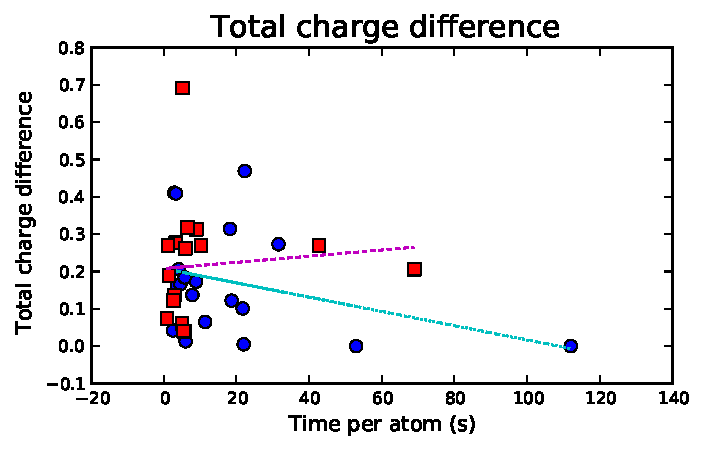
\includegraphics[width=\textwidth]{img/graphs/3a_01.pdf}
\caption{Total charge difference in relation to the average time used per atom.}
\figlab{graph_correlation_1}
\end{subfigure}%
~
\begin{subfigure}[t]{0.48\textwidth}
\centering
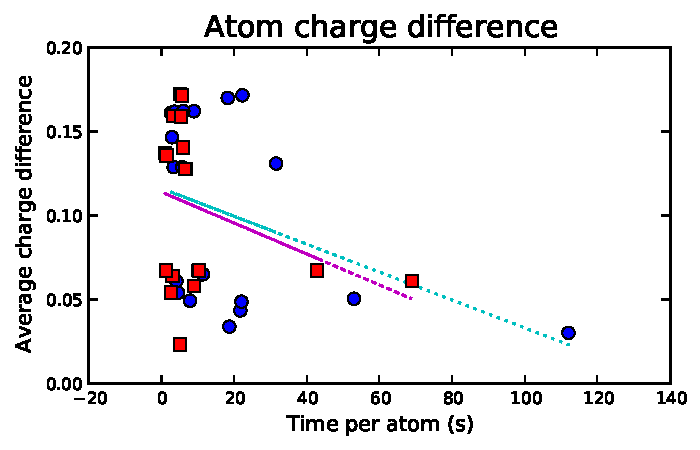
\includegraphics[width=\textwidth]{img/graphs/3a_00.pdf}
\caption{Average charge difference per atom in relation to the average time used per atom.}
\figlab{graph_correlation_2}
\end{subfigure}%
\\[1em]
\begin{subfigure}[t]{0.48\textwidth}
\centering
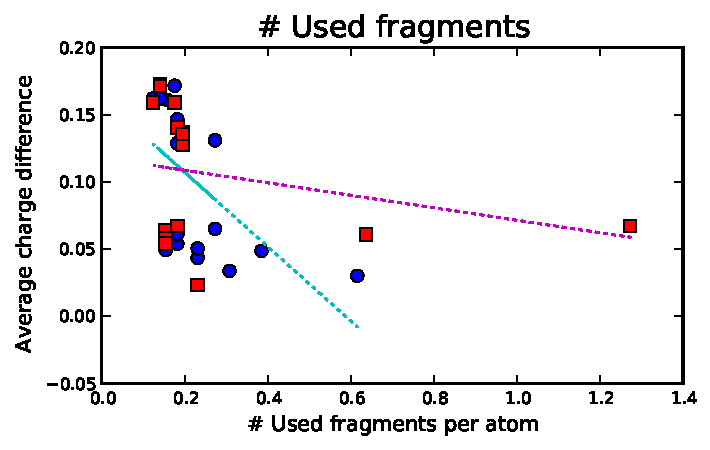
\includegraphics[width=\textwidth]{img/graphs/3a_02.pdf}
\caption{Average charge difference per atom in relation to the number of used fragments per atom.}
\figlab{graph_correlation_3}
\end{subfigure}%
~
\begin{subfigure}[t]{0.48\textwidth}
\centering
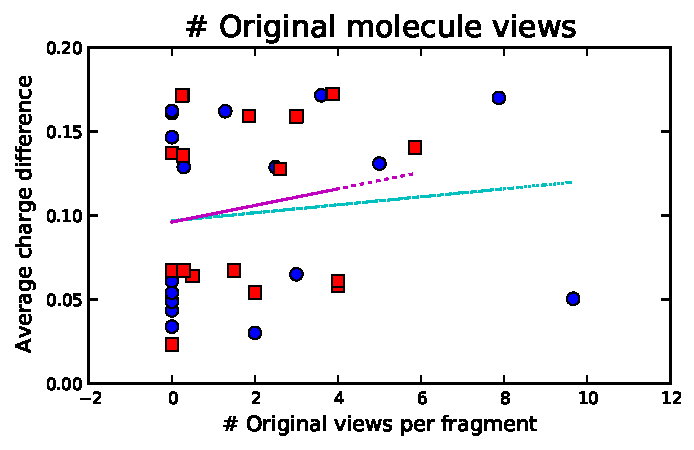
\includegraphics[width=\textwidth]{img/graphs/3a_03.pdf}
\caption{Average charge difference per atom in relation to the number of original molecule views per selected fragment.}
\figlab{graph_correlation_4}
\end{subfigure}
\caption{Presumed correlations between user studies outcomes. The blue circles are data points gathered from the consuming version, the red squares come from the producing version.}
\figlab{graph_correlation}
\end{figure}

However, as one can see almost immediately, there does not appear to be any correlation between any of the graphs shown in \figref{graph_correlation}. Even when the most extreme outliers are removed, the data points are still widely scattered and no correlation can be observed.

When taking a look at \figref{graph_correlation_1} and \figref{graph_correlation_2}, it does appear that the parameterisations the most time has been spent on are amongst the best rated. However, they are not \emph{the} best rated, and may just be outliers as they are found in isolation from the rest of the points. Furthermore, for the producing version, the users that spent the most time are not performing better than average, but these may still be outliers. A larger test group would be needed to confirm the (lack of) correlation here.

Just like is the case for the charge differences, the extremes in the number of used fragments are among the best results~(see \figref{graph_correlation_3}). However, it may also be the case here that these points are just outliers, and more experimentation is needed to be able to observe any real trend.

For the number of original molecule views, the results are the most widespread~(see \figref{graph_correlation_4}). It appears that viewing many original molecules has absolutely no effect on the quality of the parameterisation result. Furthermore, the best results for both the consuming and producing version of \oframp{} are obtained by users who did not check a single original molecule. This is an interesting observation, as it is believed that, in order to judge if a fragment is a good match, one needs to see the fragment in the context of its originating molecule. However, again, more experimentation is needed to show if there truly is no correlation between the number of original fragment views and the quality of the resulting charge.

The data shown in \figref{graph_correlation} was considered to be the most likely to have any form of correlation. It is still possible, however, that there is some correlation between any other combination of observed parameters, although this seems unlikely. Nevertheless, more experimentation is needed to be able to identify any true correlation, or to prove there is none at all.

\chapter{System requirements}
\chlab{requirements}

In order to be able to run \oframp, certain system requirements need to be met. We discuss the requirements for both the user (\secref{client_req}) and the servers (\secref{server_req}) in this chapter.


\vspace{-.1cm}
\section{Client requirements}
\seclab{client_req}
In order to be able to use \oframp, a modern browser needs to be used. There are no hardware requirements, other than those of the browser that is used to access the system. We provide support for the following browsers:

\lfootnotetext{chrome}{\url{http://chrome.google.com/}}
\lfootnotetext{ie}{\url{http://windows.microsoft.com/en-us/internet-explorer/download-ie}}
\lfootnotetext{firefox}{\url{http://www.mozilla.org/firefox/‎}}
\lfootnotetext{opera}{\url{http://www.opera.com/download‎}}
\lfootnotetext{safari}{\url{http://support.apple.com/downloads/\#safari}}

\noindent
\begin{minipage}[t]{0.5\textwidth}
\textbf{Partially supported browsers}:\vspace{.5em}

\begin{tabular}{|l|l|}
\hline
\textbf{Browser name} & \textbf{Min. version} \\\hline
Google Chrome\lfootnoteref{chrome} & 1 \\\hline
Internet Explorer\lfootnoteref{ie} & 7 \\\hline
Mozilla Firefox\lfootnoteref{firefox} & 4 \\\hline
Opera\lfootnoteref{opera} & 12 \\\hline
Safari\lfootnoteref{safari} & 5 \\\hline
\end{tabular}
\end{minipage}
\begin{minipage}[t]{0.5\textwidth}
\textbf{Fully supported browsers}:\vspace{.5em}

\begin{tabular}{|l|l|}
\hline
\textbf{Browser name} & \textbf{Min. version} \\\hline
Google Chrome\lfootnoteref{chrome} & 25 \\\hline
Internet Explorer\lfootnoteref{ie} & 10 \\\hline
Mozilla Firefox\lfootnoteref{firefox} & 25 \\\hline
- & - \\\hline
Safari\lfootnoteref{safari} & 7 \\\hline
\end{tabular}
\end{minipage}

Note that no version of the Opera\lfootnoteref{opera} browser is full supported. This is currently not possible due to the fact that, in that browser, mouse gestures are automatically bound to right mouse click and drag actions. As, in \oframp, these actions are used to make multi-atom selections, it is not possible to provide complete support for the Opera browser.

The system has been mostly tested and implemented using Google Chrome\lfootnoteref{chrome}. It is therefore recommended to use the latest version of that browser, in order to get the best experience.



\section{Server requirements}
\seclab{server_req}
As discussed before, \oframp{} consists of three systems: \oapoc{} for retrieving the atom positions, \omfraf{} for getting the fragments, and \oframp{} itself, which is the web service the user connects to. For the best results, it is advised to run all of these systems on separate servers, as both \oapoc{} and \omfraf{} have to perform computationally intensive tasks.

For \oframp, it is not necessary to be run on a server with very high performance. This server basically only needs to serve two \verb|HTML| pages, a few images, and some \verb|CSS| and \verb|JavaScript| files. \oapoc{} and \omfraf, on the other hand, are a different story, as they perform tasks that are both computationally and memory-wise intensive. Even though the processes are currently not parallelised, running the systems on multi-core machines will help with simultaneous processing of multiple users.

\lfootnotetext{oapoc_only}{Only for \oapoc}
\lfootnotetext{omfraf_only}{Only for \omfraf}

\noindent
\begin{table}[h!]
\begin{center}
\begin{tabular}{|p{.45\linewidth}|p{.45\linewidth}|}
\hline
\oframp & \oapoc / \omfraf \\\hline
Simple web server & Good web server \\
Single-core & Multi-core w/ high single-thread performance \\
100MB RAM & 1GB RAM \\
Apache (or similar) & Apache (or similar) \\
PHP 4 (or newer) & Python 2.7 \\
 & Django 1.4 \\
 & Open Babel 2.3.2\lfootnoteref{oapoc_only} \\
 & LEMON Graph Library 1.3\lfootnoteref{omfraf_only} \\\hline
\end{tabular}
\end{center}
\caption{Requirements for the different systems.}
\label{server_req}
\end{table}

Table~\ref{server_req} shows the requirements for the different servers. Note that a different configuration with a simpler server for \oapoc{} or \omfraf{} may also work, but might not give the desired performance. Furthermore, different software versions might work as well, but have not been tested.

\chapter{Setting up \oframp}
\chlab{setup}

\lstset{language=sh, frame=single, basicstyle=\ttfamily\small, breaklines=true}

When one wants to set up the \oframp{} system, it should be made sure that the requirements presented in \secref{server_req} are met. Then, one first needs to set up \oapoc{} and \omfraf{}, after which \oframp{} can be properly configured. This chapter will contain detailed instructions on the complete process, following which the set up should be easy.



\section[\oapoc]{Setting up \oapoc}
When setting up \oapoc, first, \verb|Open Babel| should be downloaded\footnote{\url{http://openbabel.org/wiki/Get_Open_Babel}}. Make sure to install the right version for your operating system, and follow the installation instructions that are provided on the download page. Once \verb|obabel| has been installed, the source code of \oapoc{} needs to be downloaded:
\begin{lstlisting}
$ git clone git@github.com:jimivdw/OAPoC.git <target>
\end{lstlisting}
Now, your web server (e.g. \verb|Apache|) needs to be configured such that \oapoc{} can be reached through the internet.

Everything should be up and running now. This can be validated by navigating with your browser to the configured root URL of your \oapoc{} instance, and submitting a simple MDS (e.g. `CCC'). If something fails, try to look at the configuration in \verb|<target>/atompos/atompos/main/util.py|, and see if anything should be changed there. This should generally not be the case, but might be necessary for some operating systems.



\section[\omfraf]{Setting up \omfraf}
Before one can set up \omfraf, the \verb|LEMON| graph library needs to be downloaded\footnote{\url{http://lemon.cs.elte.hu/trac/lemon/wiki/Downloads}} and installed following the installation instructions on the download page. Once this is done, \omfraf's source code should be downloaded:
\begin{lstlisting}
$ git clone git@github.com:jimivdw/OMFraF.git <target>
\end{lstlisting}
Next, the \verb|mop| system should be initialized. This can be done by executing the following commands:
\begin{lstlisting}
$ cd <target>
$ git submodule init
$ git submodule update
$ cd src/bin/mop/
\end{lstlisting}
Now, follow the compilation instructions present on the \verb|mop| project page\footnote{\url{https://github.com/melkebir/mop}}. Just like for \oapoc, configure your web server such that \omfraf{} can be reached through the internet.

You can now validate if everything works by navigating with your browser to the configured root URL of your \omfraf{} instance, and checking if repositories can be retrieved. Again, when something fails, one can try to look at the configuration in \verb|<target>/src/omfraf/main/util.py|, and see if anything should be changed there. This should generally not be the case, but might be necessary for some operating systems.



\section[\oframp]{Setting up \oframp}
Once both \oapoc{} and \omfraf{} have been set up, it is time to initialise \oframp. First, the source needs to be downloaded:
\begin{lstlisting}
$ git clone git@github.com:jimivdw/OFraMP.git <target>
\end{lstlisting}
Next, the URLs to \oapoc{} and \omfraf{} need to be specified in the configuration file. Open the file \verb|<path>/src/static/js/OFraMP/settings.js| in your favourite editor and look for the lines that look like this:
\begin{lstlisting}[language=JavaScript]
var DEFAULT_SETTINGS = {
  oapoc: {
    url: "http://vps955.directvps.nl/OAPoC/generate/",
    loadUrl: "http://vps955.directvps.nl/OAPoC/loadATB/",
    version: "1.0"
  },

  omfraf: {
    url: "http://vps955.directvps.nl/OMFraF/load/",
    repoUrl: "http://vps955.directvps.nl/OMFraF/repos/",
    generateUrl: "http://vps955.directvps.nl/OMFraF/generate/",
    version: "1.0"
  },
  // ...
};
\end{lstlisting}
Make sure to replace all URLs with those where your \oapoc{} and \omfraf{} servers are located. Now, one last time, configure your web server such that \oframp{} can be reached through the internet. Everything should be up and running, and \oframp{} is ready to be used.

\chapter{User studies instructions}
\chlab{instructions}

In this chapter, the exact instructions that have been provided to the user studies participants can be found. Note that these are the instructions for the group that first did the \IDa\ version of \oframp, followed by the \IDb\ version. The other group of participants received similar instructions, but just with the URLs swapped.

Please execute the following steps in the exact order in which they are presented:
\begin{enumerate}
\item Go to OFraMP at \url{http://vps955.directvps.nl/OFraMP/n/};
\item As soon as the page has been loaded, click the `Start demo' button;
\item Follow the instructions given to you by the demo, and finish the parameterisation of the demo molecule (does not need to be perfect, just make sure every atom has a charge assigned);
\item Now, either reload the page or click the `New molecule' button at the top of the page;
\item Insert the following into the text input field: \textbf{10321}. This number represents an ATB ID, which we use here as it is easier to insert than a SMILES or InChI string. It represents 1,3-propandiol (PDO), a molecule with a total net charge of \textbf{0.0};
\item Make sure the repository is set to \textbf{arbitrary\_qm1} (an arbitrary selection of QM1 molecules from the ATB) and the shell size to \textbf{1}; then click the `Submit' button;
\item Fully parameterise the molecule, just like you did in the demo. This time, try to make it as good as possible and try to make the charges add up to the total net charge of the molecule. Feel free to consult the Help page if you need more detailed information;
\item \underline{Make sure to download the result LGF file} using either the `Download LGF' button in the `Fully parameterised' popup, or the `Download' button at the top of the page;
\item Now, enter a new molecule \textbf{16978} (\_V3M, total net charge of \textbf{-1.0}) and repeat steps 6 through 8. Again, \underline{remember to download the result file};
\item Please evaluate \emph{this version} of the system at \url{http://vps955.directvps.nl/OFraMP/nq/}. \underline{Try to focus as much as you can on the user interaction aspect}. Note that statements are ranked on a scale of 1 (strongly \emph{dis}agree) to 5 (strongly agree);
\item As soon as you have submitted the questionnaire, please go to the second version of OFraMP, available at \url{http://vps955.directvps.nl/OFraMP/s/};
\item Quickly take the demo again, in order to get to know this version and the differences with the other;
\item Fully parameterise the molecule \textbf{13913} (1h-imidazol-2-amine (2AI), total net charge of \textbf{0.0}). Again, make sure the repository and shell size are set to the values shown in step 6, and please \underline{download the result file as soon as you are done};
\item Parameterise one final molecule: \textbf{17738} (borrelidin (\_VOQ), total net charge of \textbf{-1.0}), with the same repository and shell size, and also \underline{download this one's result};
\item Please evaluate \emph{this version} of the system at \url{http://vps955.directvps.nl/OFraMP/sq/}. Again, \underline{try to focus as much as you can on the user interaction aspect}. Note that statements are, again, ranked on a scale of 1 (strongly \emph{dis}agree) to 5 (strongly agree);
\item Finally, please answer some general questions at \url{http://vps955.directvps.nl/OFraMP/q/}.
\end{enumerate}
Good luck, and thanks again for participating in the user studies.

\chapter{User studies questionnaires}
\chlab{questionnaires}

This chapter will contain the questionnaires that the experiment participants were asked to complete\ldots

\nlipsum

\chapter{Graphs}
\graphicspath{ {/home/jimi/Dropbox/MasterProject/results/graphs/} }
\tolerance=1000000
\centering
\includegraphics{1a_00.pdf}
\includegraphics{1a_01.pdf}
\includegraphics{1a_02.pdf}
\includegraphics{1a_03.pdf}
\includegraphics{1b_00_00.pdf}
\includegraphics{1b_00_01.pdf}
\includegraphics{1b_00_02.pdf}
\includegraphics{1b_00_03.pdf}
\includegraphics{1b_01_00.pdf}
\includegraphics{1b_01_01.pdf}
\includegraphics{1b_01_02.pdf}
\includegraphics{1b_01_03.pdf}
\includegraphics{1b_02_00.pdf}
\includegraphics{1b_02_01.pdf}
\includegraphics{1b_02_02.pdf}
\includegraphics{1b_02_03.pdf}
\includegraphics{1b_03_00.pdf}
\includegraphics{1b_03_01.pdf}
\includegraphics{1b_03_02.pdf}
\includegraphics{1b_03_03.pdf}
\includegraphics{2a_00.pdf}
\includegraphics{2a_01.pdf}
\includegraphics{2a_02.pdf}
\includegraphics{2a_03.pdf}
\includegraphics{2a_04.pdf}
\includegraphics{2a_05.pdf}
\includegraphics{2a_06.pdf}
\includegraphics{2a_07.pdf}
\includegraphics{2a_08.pdf}
\includegraphics{2a_09.pdf}
\includegraphics{2a_10.pdf}
\includegraphics{2a_11.pdf}
\includegraphics{2a_12.pdf}
\includegraphics{2a_13.pdf}
\includegraphics{2a_14.pdf}
\includegraphics{2b_00.pdf}
\includegraphics{2b_01.pdf}
\includegraphics{2b_02.pdf}
\includegraphics{2b_03.pdf}
\includegraphics{2b_04.pdf}
\includegraphics{2b_05.pdf}
\includegraphics{2b_06.pdf}
\includegraphics{2b_07.pdf}
\includegraphics{2b_08.pdf}
\includegraphics{2b_09.pdf}
\includegraphics{2b_10.pdf}
\includegraphics{2b_11.pdf}
\includegraphics{2b_12.pdf}
\includegraphics{2b_13.pdf}
\includegraphics{2b_14.pdf}
\includegraphics{2c_00.pdf}
\includegraphics{2c_01.pdf}
\includegraphics{2c_02.pdf}
\includegraphics{2c_03.pdf}
\includegraphics{2c_04.pdf}
\includegraphics{2c_05.pdf}
\includegraphics{2c_06.pdf}
\includegraphics{2c_07.pdf}
\includegraphics{2c_08.pdf}
\includegraphics{2c_09.pdf}
\includegraphics{2c_10.pdf}
\includegraphics{2c_11.pdf}
\includegraphics{2c_12.pdf}
\includegraphics{2c_13.pdf}
\includegraphics{2c_14.pdf}
\includegraphics{2d_00_00.pdf}
\includegraphics{2d_00_01.pdf}
\includegraphics{2d_00_02.pdf}
\includegraphics{2d_00_03.pdf}
\includegraphics{2d_01_00.pdf}
\includegraphics{2d_01_01.pdf}
\includegraphics{2d_01_02.pdf}
\includegraphics{2d_01_03.pdf}
\includegraphics{2d_02_00.pdf}
\includegraphics{2d_02_01.pdf}
\includegraphics{2d_02_02.pdf}
\includegraphics{2d_02_03.pdf}
\includegraphics{2d_03_00.pdf}
\includegraphics{2d_03_01.pdf}
\includegraphics{2d_03_02.pdf}
\includegraphics{2d_03_03.pdf}
\includegraphics{2d_04_00.pdf}
\includegraphics{2d_04_01.pdf}
\includegraphics{2d_04_02.pdf}
\includegraphics{2d_04_03.pdf}
\includegraphics{2d_05_00.pdf}
\includegraphics{2d_05_01.pdf}
\includegraphics{2d_05_02.pdf}
\includegraphics{2d_05_03.pdf}
\includegraphics{2d_06_00.pdf}
\includegraphics{2d_06_01.pdf}
\includegraphics{2d_06_02.pdf}
\includegraphics{2d_06_03.pdf}
\includegraphics{2d_07_00.pdf}
\includegraphics{2d_07_01.pdf}
\includegraphics{2d_07_02.pdf}
\includegraphics{2d_07_03.pdf}
\includegraphics{2d_08_00.pdf}
\includegraphics{2d_08_01.pdf}
\includegraphics{2d_08_02.pdf}
\includegraphics{2d_08_03.pdf}
\includegraphics{2d_09_00.pdf}
\includegraphics{2d_09_01.pdf}
\includegraphics{2d_09_02.pdf}
\includegraphics{2d_09_03.pdf}
\includegraphics{2d_10_00.pdf}
\includegraphics{2d_10_01.pdf}
\includegraphics{2d_10_02.pdf}
\includegraphics{2d_10_03.pdf}
\includegraphics{2d_11_00.pdf}
\includegraphics{2d_11_01.pdf}
\includegraphics{2d_11_02.pdf}
\includegraphics{2d_11_03.pdf}
\includegraphics{2d_12_00.pdf}
\includegraphics{2d_12_01.pdf}
\includegraphics{2d_12_02.pdf}
\includegraphics{2d_12_03.pdf}
\includegraphics{2d_13_00.pdf}
\includegraphics{2d_13_01.pdf}
\includegraphics{2d_13_02.pdf}
\includegraphics{2d_13_03.pdf}
\includegraphics{3_00.pdf}
\includegraphics{3_01.pdf}
\includegraphics{4a_00.pdf}
\includegraphics{4a_01.pdf}
\includegraphics{4a_02.pdf}
\includegraphics{4a_03.pdf}
\includegraphics{4a_04.pdf}
\includegraphics{4a_05.pdf}
\includegraphics{4a_06.pdf}
\includegraphics{4a_07.pdf}
\includegraphics{4a_08.pdf}
\includegraphics{4a_09.pdf}
\includegraphics{4a_10.pdf}
\includegraphics{4b_00.pdf}
\includegraphics{4b_01.pdf}
\includegraphics{4b_02.pdf}
\includegraphics{4b_03.pdf}
\includegraphics{4b_04.pdf}
\includegraphics{4b_05.pdf}
\includegraphics{4b_06.pdf}
\includegraphics{4b_07.pdf}
\includegraphics{4b_08.pdf}
\includegraphics{4b_09.pdf}
\includegraphics{4b_10.pdf}
\tolerance=1000

\chapter{Comments}

In this chapter, all comments on the two versions of the system that were given during the user studies can be found. The most important of these, as well as the general opinion, are discussed in \chref{results}.

\section{\oframp{} naive}
\subsection{First}
\subsubsection{Positive comments on the chemistry aspect}
\begin{itemize}
\item Quickly selecting arbitrary fragments, looking at the compounds they originate from and iteratively redoing partial charge assignment to get "it right" is good

\item A good variety and potential charge groups available

\item It is a fast way to estimate atomic charges for the unparametrised molecules. It is also quite informative regarding the differences of the same groups in different environments, or different solutions for identical fragments.

\item Extremely useful to have a tool to screen for possible sets of charges for a given fragment in a database with pre-equilibrated charges!

Nice representation of molecules and fragments, see below for a few suggestions for possible future extensions.

\end{itemize}


\subsubsection{Negative comments on the chemistry aspect}
\begin{itemize}
\item I'm missing out on some intelligence in the interface. What about when the compound contains two identical subunits, could the system point me to it and apply a fragment to both? Could the system take the context (environment) of the fragment selected into account apart from setting shell size, e.a. does the oxygen link to a neighboring phosphate or carbon for instance. Makes a difference in the partial charge it gets. Perhaps sort available fragment to reflect this

\item When many atoms selected, there was no group that could be selected for charge assignment; many charge options possible, how do we know which one is correct/the best; maybe adding confidence factor would help

\item I found that there are several possible solutions for the fragments in the identical context. The question is - which one is to use? Another important question would be how good are the offered charges and what is the impact of mixing parts from different molecules which clearly have different ideas about charge values for certain atom types. I think some ranking could be introduced in sense of adding some flag to more reliable set of charges (by reliable, I mean something that is derived following certain standard procedures).

\item - It would be very useful to have the possibility to switch to a representation that includes hydrogens explicitly (i.e., to see charges on hydrogens and hydrogen-bound atoms explcitly). Especially charges on hydrogens bound to any atom {\textbackslash}other{\textbackslash} than carbon would be good to be visualized (and then have an option to switch between representation with and without carbond-bound atoms?)

- It would be very nice to have the possibility to distribute error in net charge of molecule (as defined by user) over a selected set or all atoms of the molecule (to be selected by user as well).

\end{itemize}


\subsubsection{Positive comments on the user interaction aspect}
\begin{itemize}
\item The interface is very clear, no hidden options elaborate menu's and so on. I could start working right away.

\item Clear labels, clear information about the charges, nice clear layout

\item It is a rather user friendly interface and I did not have any major problems with it, except when my connection seemed to unusually slow so I couldn't load the available fragments for inspection.

\item Many very useful funcionalities.

Fast generation of fitting fragments.

The possibility to easily check the molecule from which a given fragment originates is really nice.

Extensive help function.

Various coloring schemes to warn for atoms for which no fragments are found, overlapping atoms, etc.

\end{itemize}


\subsubsection{Negative comments on the user interaction aspect}
\begin{itemize}
\item I would always like to see a window indicating the total charge of the system yet parameterized. Also when the system fully parameterized, show the final statistics. Can the system track consistency in real time? perhaps give helpful pointers for parts of the molecule that are not properly parameterized? 

\item The pop-up window after the completion of molecule is confusing; difficult to 'return' to a previous page

\item It is not so easy to answer this question after just 2 molecules, it would probably take some time to figure out what is annoying in the every day usage.

\item - Two small suggestions for the demo:

 I 'by accident' found out that after starting the demo, I had to click on the window to have a demo-molecule appear, shouldn't that be in the instructions? And maybe add something like "Swipe with two fingers over mouse pad when scroll wheel is missing" to the demo?

-  I (quickly) found out that I could/had to use arrow keys to scroll down in the menu with selected fragments, when many of them were found and I wanted to look at many of them as well.

-  I was confused by the light color of the atoms in (orange highlighted) fragments: I thought they would not be part of the fragment or so, maybe you could indicate charges that have been assigned already with another color (red font?) instead of changing the color of the atoms)? It is just a suggestion.

- Could you in the menu "attempting to assign a new charge to an already charged atom"  easily highlight the atom that is actually considered with a separate color? That would be very helfpul in the (regularly occurring) cases in which a fragment contains more than one atom with the same atom name.

- It would be very nice to be able to change the default position of the pop-up after clicking "show molecule" (i.e. to have the pop-up not overlapping with the structure of the molecule to be paratemerized).

- From a user perspective, it would be ideal to be able to see for already selected charges to which fragment they belong, e.g. when selecting a fragment in the big molecule, it may have overlap with earlier assigned fragments, and it would be very nice if the user could see with which part of a pre-chosen fragment(s) there is overlap. I could well imagine several issues with implementation (e.g. how to color code atoms that have had overlap between different pre-chosen fragments??)

\end{itemize}


\subsubsection{Any errors that have occurred}
\begin{itemize}
\item None

\item None

\item None

\item I (Daan) encountered the following issues during the demo:

after selecting a first fragment, I selected two atoms (with control-click), for which no fragments could be selected. Then, I did not manage to unselect any of the two selected atoms, and when clicking undo, all selections disappeared and I got the demo hanging when clicking undo and clicking the menu with fragments away (the description about the fragment-menu on the right remained, and I could not make a new selection anymore, so I had to restart the demo, after which I got it hanging again following the same sequence of my selections (I would be happy to show this, this seems to be a bug in the demo; I hope I am wrong.)

\end{itemize}


\subsubsection{General comments}
\begin{itemize}
\item None

\item None

\item None

\item Great achievement and a very nice application and user-interface!



One tiny remark on the questionnaire:  I almost filled in the first part of the questionnaire on the opposite scale, maybe put more emphasis on the remark Please rate the following statements on a scale of 1 (strongly disagree) to 5 (strongly agree)."  ?   (Or show 5  4  3  2  1  n/a) 

\end{itemize}


\subsection{Second}
\subsubsection{Positive comments on the chemistry aspect}
\begin{itemize}
\item It is good to have the possibility to decide which atoms should compose a fragment, and in which direction try to increase the fragment to look for.



\item The ease with which similar portions of different molecules can be identified.

\item The chemical context was well-defined, and the list of alternatives was extensive

\item In short the overview of all the options for a selection of atoms really allows for a good choice of fragments, however typically the best fragment is not the first one displayed. Especially after a short while it becomes very intuitive to just start with the functional groups and then build up the rest of the molecule, with resulting charges that at least look decent.

\end{itemize}


\subsubsection{Negative comments on the chemistry aspect}
\begin{itemize}
\item It would be useful to have a system of averaging among a selected group of atoms.

\item The available fragments seem to be missing some common functional groups. To be chemically relevant the buffer region surrounding fragments must be larger to ensure a degree of independence between fragments. 

\item Some fragments did not have values I would have expected. Inserting them by hand would have been convenient

\item It would be nice to be more capable of adapting charges for a certain atom at a later time. E.g. allow you to remove certain fragments that were used. Right now especially with the huge borredlin molecule you would have to either start all over again or keep hitting the back button. 

\end{itemize}


\subsubsection{Positive comments on the user interaction aspect}
\begin{itemize}
\item The list of fragments on the side is very useful, together with the automated updating of the window reporting the original molecule.

I liked a lot the interactive search of fragments, while selecting different groups of atoms.

\item I think the user interface is very good: responsive, intuitive, easy to lean and use. 

\item The information needed pops up when needed

\item The user interface was great and easy to use. It's use is very intuitive and it's lightning fast.

\end{itemize}


\subsubsection{Negative comments on the user interaction aspect}
\begin{itemize}
\item In the side panel of the fragments, it would be more handy to display the entire molecule, in which the fragment is highlighted.

It would be more practical to have the possibility to change the atom by hand, without selecting any fragment, in case no suitable fragment has been found.

A preliminary search for big fragments, as present in OFraMP version s, could speed up the parametrization process.

\item Drag to select multiple atoms simultaneously.  It is impractical to keep track of net charge for large molecules. 

\item The list of fragments was not scrollable, reducing 100+ options to only a few

\item Again, I think a great addition to the system would be the use of color coding for the different elements.

\end{itemize}


\subsubsection{Any errors that have occurred}
\begin{itemize}
\item None

\item None

\item None

\item None

\end{itemize}


\subsubsection{General comments}
\begin{itemize}
\item None

\item None

\item None

\item None

\end{itemize}


\section{\oframp{} smart}
\subsection{Second}
\subsubsection{Positive comments on the chemistry aspect}
\begin{itemize}
\item -

\item All assignment done almost without user's input

\item Finding the matching fragment was faster than in the previous version.

\item As the previous version (version n), it is great to have an interface for automated selection of molecular fragments and atomic charges in hand! This one is even easier to use, but this is probably due to a functionality that I miss when compared to the previous version (see below).

\end{itemize}


\subsubsection{Negative comments on the chemistry aspect}
\begin{itemize}
\item I was missing out on the true process of fragment based assembly. I often thought I could do better of the particular fragment in context of the whole compound but did want to go to accept/reject/undo cycles. 

\item How are the groups assigned? The same molecule starts optimizing from different parts at different trials. Sometimes no optimal solution available. 

\item I would really like if I could see all the charges in the context molecule rather than just for the fragment. It would help in making a better guess for the neighbouring fragment, considering the multiple options. 

\item I prefer a scroll down menu on the right side, such that I can easily compare different possible fragments. Now I have to click back and forth between different possbilities (to compare them), and that makes this version in fact less user friendly from the chemist's point of view than version n.

Furthermore, most of my remarks on what is good and on what might be improved, as filled in in evaluation of version n, holds true for the current version (s) as well.

\end{itemize}


\subsubsection{Positive comments on the user interaction aspect}
\begin{itemize}
\item The system making suggestions and taking the lead in the process of parametrization is helpful and helps me getting "up and running" quicker. 



\item Nice clear layout

\item The automatic assignation of the fragment charge speeds up the procedure.

\item See my first answer.

\end{itemize}


\subsubsection{Negative comments on the user interaction aspect}
\begin{itemize}
\item Opposed to the other interface I consider this one to be more of a "black box" Making suggestions is great but I would like tot see the window displaying the alternative fragments available at each suggestion as well as na overal status window show total charge of the system assigned so far and more. 

\item The pop-up window at the end confusing - it covers the result. Difficult to return to previous page/settings

\item Although this automatic selection of the fragment can make choice a bit easier, in cases of larger molecules with different functional groups, it gets more tedious because every rejection results with blind next guess. Perhaps after the first rejection it would be nice to have the menu with all the molecules with the given fragments as in the previous versions.

\item Most of my remarks on what is good and on what might be improved, as filled in in evaluation of version n, holds true for the current version (version s) as well.

My main suggestion would be to let the pop-up menu, after clicking on 'view original' (either in version s or n), pop up beside of the molecule in the main menu, and not let them overlap (as it is now, which means that I constantly have to drag it beside of the molecule in the main menu).

Would it maybe be possbile to combine both functionalities of s and n? I.e., to include both the availability of the buttons below (as in this version s), and the scroll menu on the right?

\end{itemize}


\subsubsection{Any errors that have occurred}
\begin{itemize}
\item None

\item None

\item Sometimes after changing the selection of the fragment, the system would not change the charges anymore, but that could've been my fault too (perhaps I did something wrong unaware of it).

\item None

\end{itemize}


\subsubsection{General comments}
\begin{itemize}
\item None

\item None

\item None

\item Include the demonstration of the possibility to click on and adapt atoms in the demo.

\end{itemize}


\subsection{First}
\subsubsection{Positive comments on the chemistry aspect}
\begin{itemize}
\item The search for the fragments, starting from the biggest to the smallest one found in the repository; the possibility to visualize the query molecule and the original molecule where the fragment has been found.

\item The automated search for possible fragments is helpful. 

\item The system shows the molecules the fragments are chosen from, allowing to get the proper chemical context of the fragment.

\item At least the first few fragments it proposes for a certain part of the molecule look pretty good. The selection details screen really allows for quickly viewing all the necessary information. It allowed for rapidly obtaining a seemingly okay charge distribution for the second molecule.

\end{itemize}


\subsubsection{Negative comments on the chemistry aspect}
\begin{itemize}
\item It should be possible to visualize more fragments at the same time, in order to choose the best one. When adding a new fragment, it should be possible to not overwrite charges that have been previously parametrized.

\item The local environments surrounding matched fragments is not large enough to ensure that fragments are independent. 

\item When looking for the 'best' fragment description, aal fragments have to be accepted or rejected, without knowing what other fragments might be coming. As such the choice becomes a bit arbitrary.

\item The proposed fragment quality goes rapidly down hill from just the first few fragments and the proposed fragments become quite inaccurate, especially for small groups such as just a CH3 group. This generally resulted in me having to hit the undo button about 10 times to get back to the first proposed one. It would be better to just have an overview of all available fragments. Averaging the charges of several fragments for a certain part of the molecule also worries me, especially since there is no option to NOT average the charge for certain atoms instead of averaging them with the new fragment.



The system also does not take into acount molecular symmetry for the 1,3-propanediol, which results in using 1-butanol for the CH2(OH) and the CH2, but not for the other CH2(OH), while in fact these groups are identical. 



Finally I think that "matching the total charge" is an inappropriate way for judging the quality of the obtained partial charges.

\end{itemize}


\subsubsection{Positive comments on the user interaction aspect}
\begin{itemize}
\item Easy interface and nice way to submit the query molecule

\item The user interface is simple to lean and use. 

\item the system runs smoothly, all interactions are quite intuitive.

\item It's incredibly easy to use. The selection details screen is very useful. The molecule and the proposed fragment are illustrated very well.

\end{itemize}


\subsubsection{Negative comments on the user interaction aspect}
\begin{itemize}
\item Explicit visualization of double/triple bonds would make the comparison between fragments and molecule more intuitive.

A window that describes the proposed fragment in the original molecule should be always present and updated when a fragment is discarded.

It would be useful to have the possibility to select again a fragment that has been previously discarded.

\item When a potential match is rejected the update of the selected fragment isn't obvious i.e. it appears as if nothing has changed. Showing multiple possible fragments would speed up the fragment selection process. Showing the net charge on each fragment and on the paramaterized portion of the molecule would make it much simpler to keep track of net charge. 

\item the selection detail window is not completely obvious at first sight

\item What I really would prefer is that the interface uses at least some idea of the standard color marking for atoms (e.g. red for oxygen, blue for nitrogen), since this is generally how these molecules are viewed by chemists and it makes it easier to see if a fragment is a match just by looking at it once.

\end{itemize}


\subsubsection{Any errors that have occurred}
\begin{itemize}
\item None

\item None

\item None

\item None

\end{itemize}


\subsubsection{General comments}
\begin{itemize}
\item None

\item None

\item None

\item None

\end{itemize}


\section{General comments}
\subsection{Naive first}
\subsubsection{Preferred version}
\begin{itemize}
\item Naive

\item Naive

\item Naive

\item Naive

\end{itemize}


\subsubsection{Explanation for preferred version}
\begin{itemize}
\item More control over fragment assembly proces. 

\item To be honest I liked both of them, I liked seeing all the available charge groups and picking one rather than having the groups assigned blind (version 2)

\item I found it easier to use and it felt like I have more control over it. The second version requires a lot of clicking back and forth because I can't see what is the next guess and it's not necessarily better than the first one. And it gets confusing when the fragment selection is being changed, I don't find the second version very responsive in that sense. Basically, I find the first version more flexible.

\item I prefer version n, because I prefer the scroll down menu on the right to more easily compare possible fragment selections.

\end{itemize}


\subsubsection{Functionality of the other (not preferred) version that should be included in the preferred one}
\begin{itemize}
\item Automatically "walking" through the fragment assembly proces for the compound but keeping the window with alternate fragment options available. 

\item I think it would be nice to have the groups assigned automatically (version 2), but also having the others potential charge groups visible on the side (as in version1)

\item None

\item Combination of n and s (see my comments to questionnaire s).

\end{itemize}


\subsubsection{Suggestions for additions to the preferred versions}
\begin{itemize}
\item Small window with overal statistics. Like total charge of the system while it is being parameterized and even the effect of a different choice on the total charge. That would introduce a bit of "game like" aspects to the proces. 

\item Maybe adding the confidence score of how sure we are about the fact the the assigned charge groups are correct for our molecule. Defining the total charge at the beginning so the groups are fitted to match it would be good as well.

\item I would like to see the charges for all the atoms in the molecule, not just the fragments because it would allow a better guess of the charge set for the patching fragment, in my opinion. Just as a context. 

\item See my remarks at questionnaire n.

\end{itemize}


\subsubsection{General comments}
\begin{itemize}
\item Not more than the above and to say you did a nice job building it!

\item Nice work!

\item None

\item Excellent job, quality and functionality!

\end{itemize}


\subsection{Smart first}
\subsubsection{Preferred version}
\begin{itemize}
\item Naive

\item Naive

\item Naive

\item Naive

\end{itemize}


\subsubsection{Explanation for preferred version}
\begin{itemize}
\item The parametrization process is based on the similarity between a query compound and an already paramaterized molecule: version 1 does not practically allow a comparison between the different proposed fragments.

The graphical representation of the molecules in version 1 was less intuitive.

\item Seeing the possible fragments and the local environment of the molecule made the process much quicker. 

\item all options for fragments are given together, allowing for an informed choice

\item The overview of fragments is way more intuitive than just the "accept, reject" system. It may allow for larget throughput if the fragments found match very closely and the first proposal is correct, but in practice I found myself continually hitting undo.

\end{itemize}


\subsubsection{Functionality of the other (not preferred) version that should be included in the preferred one}
\begin{itemize}
\item The automated search for the biggest fragments as preliminary step.

\item The first fragment could be automatically suggested based on the largest possible match.

\item None

\item None

\end{itemize}


\subsubsection{Suggestions for additions to the preferred versions}
\begin{itemize}
\item None

\item Addition of net charge to potential fragments and to the currently parameterized portion of the molecule. Restriction of the minimum buffer region size to a chemically reasonable value e.g. 3. Entire molecules could be considered as potential fragments e.g. if molecule A contains molecule B as a fragment. Where possible, fragments with an integer (or near integer charge) should be preferred. Generate MD forcefield output by combining the parameters of the matched fragments.

\item I would like to know the raw charges from atb/qm, to guide my choice

\item Color coding for the different elements.



Allowing for one to more easily adjust the fragment selection afterwards.

\end{itemize}


\subsubsection{General comments}
\begin{itemize}
\item None

\item I think that the system has great potential! The user interface is very intuitive and easy to use. In order to be generally useful as a parameterization aid a few changes are required, but I suspect that the majority of the truly novel functionality (identifying matching fragments) is already present. 

\item None

\item None

\end{itemize}




\cleardoublepage

\end{document}
